\chapter{Nonpremixed Counterflow Cool Flames}\label{ch:NTC}

As reviewed in Chapter~\ref{sec:intro-NTC-generic}, the invariable existence of nonuniformities in practical combustion systems requires consideration of the coupled effects of chemistry and transport on cool flames.  Consequently, in this chapter, nonpremixed counterflow cool flames studies are presented.  The primary objective is to experimentally explore the existence of nonpremixed cool flame.  The investigation is a challenging one because of the weak reactivity and the correspondingly weak exothermicity involved.  Upon the affirmation of the exploration of the nonpremixed cool flame, characterization of the ignition and extinction behavior of the cool flame is performed and compared with computations to facilitate further studies on cool flames.

\section{Experimental Investigation}\label{sec:NTC-exp}

Dimethyl ether (DME) was selected as the fuel for the present study because it is gaseous and is one of the simplest hydrocarbons exhibiting NTC behavior.  Furthermore, detailed reaction mechanisms for low- and high-temperature DME oxidation~\cite{curran98,fischer00,curran00,zhao08} have been developed and validated for burner stabilized flames~\cite{kaiser00}, nonpremixed counterflow flame ignition~\cite{zheng05}, laminar flame speeds~\cite{qin05}, and studies using rapid compression machines~\cite{mittal08}.  This allows the computational simulation and thereby guidance and verification of the experimentation with moderate confidence. In particular, computations presented in Sec.~\ref{sec:NTC-comp} were conducted using a skeletal mechanism of $39$ species~\cite{bhagatwala15} reduced from the detailed mechanism of Zhao \emph{et al.}~\cite{zhao08}.

A schematic of the experimental setup is shown in Fig.~\ref{fig:NTC-setup}; detailed descriptions of the counterflow experimental apparatus are given in~\cite{fotache95,liu10a}.  Briefly, the apparatus consists of two vertically oriented opposing quartz nozzles with diameters of $20$ mm separated by $20$ mm.  A heated air or N$_2$ stream is issued from the upper nozzle and impinges against a room-temperature N$_2$-diluted DME steam issued from the lower nozzle.  Both upper and lower streams are shielded by coflowing N$_2$ to minimize disturbance from the environment.  In a typical counterflow ignition experiment, ignition is achieved by gradually increasing the air boundary temperature until a visible flame appears. The exit temperature, measured by a thermocouple with radiation correction~\cite{zheng06}, is then defined as the ignition temperature. Single-point laser Doppler velocimetry (LDV) is used to measure the axial flow velocity along the centerline to determine the local strain rate (velocity gradient) of the flow.

\begin{figure}[t]
  \centering
  \scriptsize
  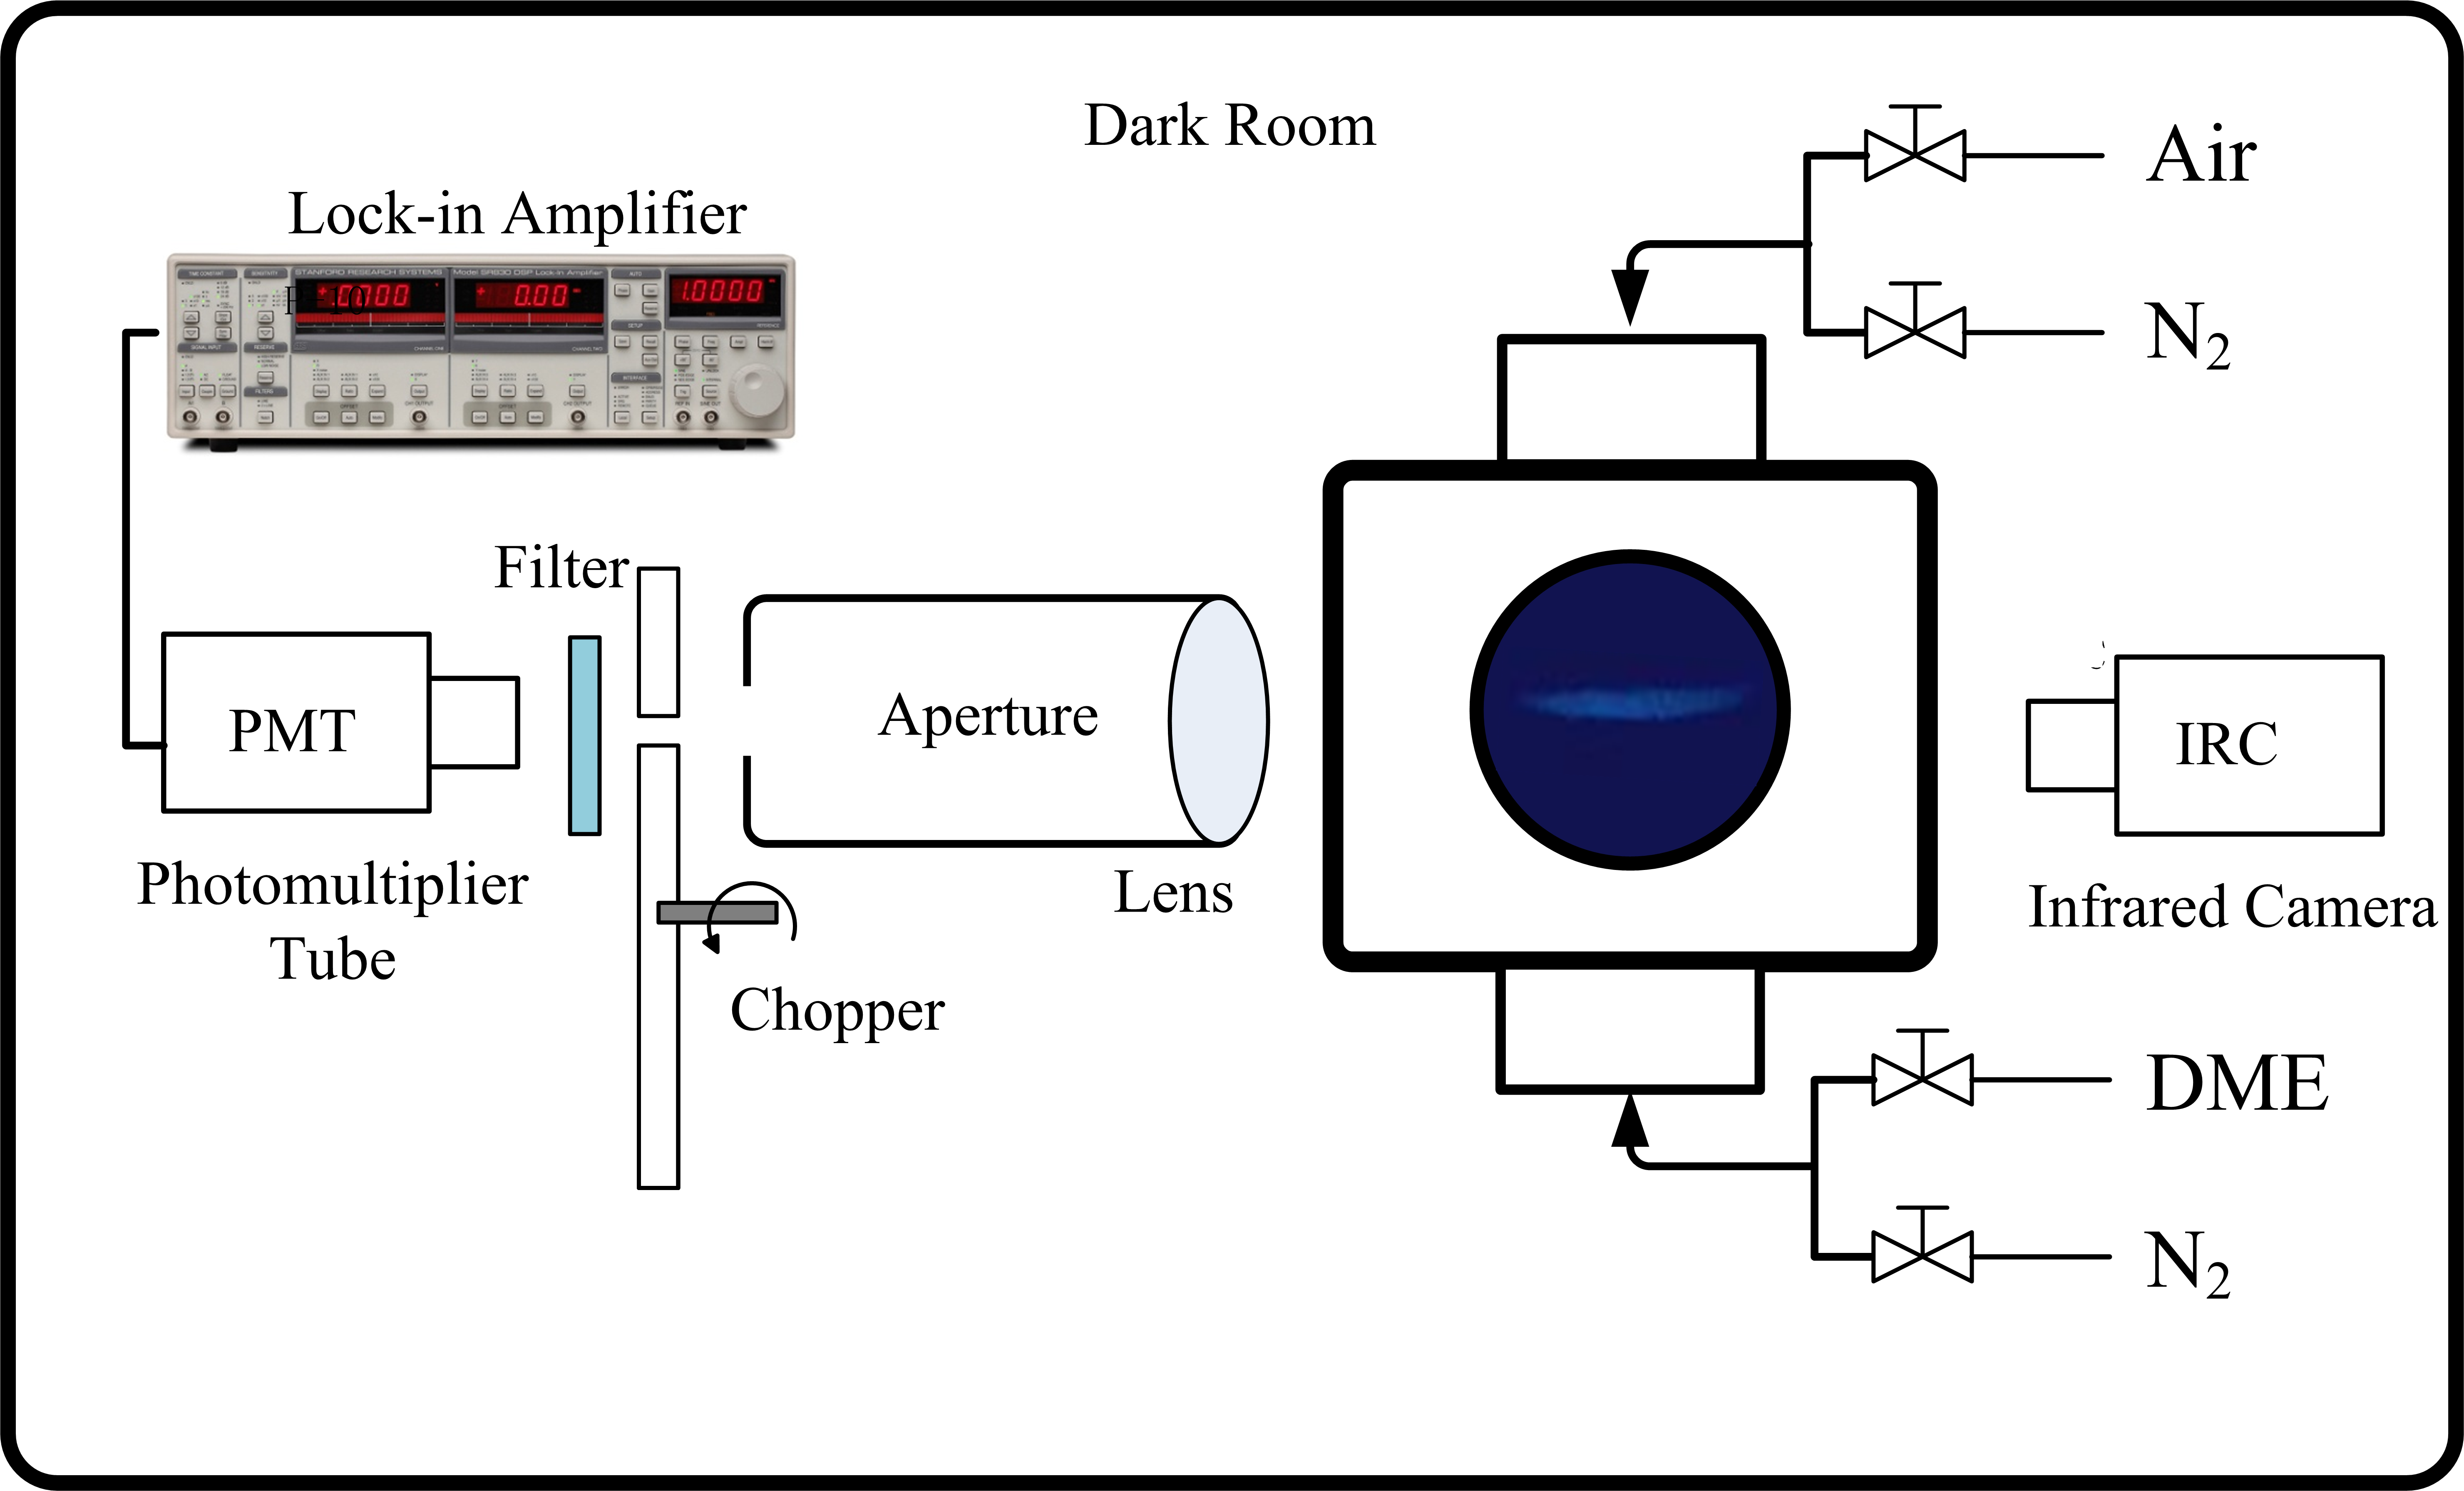
\includegraphics[width=1.0\textwidth]{ch-NTC/Experimental_Setup.png}
  \normalsize
  \caption{Schematic of the nonpremixed DME/air counterflow system for the detection of cool flames and quantification of the cool flame ignition temperatures.}
  \label{fig:NTC-setup}
\end{figure}


While the above procedure has been successfully used in previous studies of ignition and the diagnosis of the resulting flame for strongly burning flames, for which the instant of ignition can be observed visually, no bright flame or visually-detectable reaction front could be observed for the present NTC-affected ignition within the temperature range of interests ($600$-$800$ K).  Furthermore, no discernable heat release was detected by using a thermocouple, ostensibly due to the small amount of heat release from the low-temperature chemistry.  In the absence of a visible flame, it was also not clear the extent of the disturbance introduced by the thermocouple to the flow field as well as the ignition kernel.

In view of the above limitations, optical detections and measurements were chosen for this work.  A photomultiplier tube (PMT) was subsequently applied to detect any NTC-related chemiluminescence, noting that experimental studies in homogeneous systems have shown that the NTC-induced chemistry have characteristic chemiluminescence spectra, with a small amount of heat release~\cite{sheinson73,ohta91}.  These studies further showed that a large amount of formaldehyde (CH$_2$O or HCHO) is formed from the low-temperature chemistry and the pale blue chemiluminescence from CH$_2$O characterizes the associated low-temperature reaction~\cite{gaydonbook}.  Based on these characteristics, the experimental setup was designed as shown in Fig.~\ref{fig:NTC-setup}. Here a Hamamatsu 931B PMT combined with focusing lens system and a Newport filter (10BPF10-400) was used to detect the chemiluminescence corresponding to the characteristic wavelength of formaldehyde (peaks around $400$ nm) and to reduce noise light signals from the counterflow chamber. The PMT signal was then collected and processed with a SR510 lock-in amplifier to further diminish the noise.  Results based on this experimentation to demonstrate the existence of the low-temperature chemistry in the counterflow are discussed in Sec.~\ref{sec:NTC-4.1}.  This is followed by an investigation based on infrared imaging to identify the state of ignition, in Sec.~\ref{sec:NTC-4.2}. 

\section{Computational Investigation}\label{sec:NTC-comp}

As introduced in Sec.~\ref{sec:intro-NTC-nonpremixed}, the steady-state response of a one-dimensional reactive system subjected to heat loss can be studied with the S-curve analysis~\cite{lawbook}. In such an analysis, a system response such as the maximum temperature or radical concentration is monitored for variations of an imposed parameter such as the air temperature, for a given strain rate of the flow, or the system Damk\"ohler number.  A typical S-shaped response curve has a lower turning point that designates the ignition state and a upper turning point that corresponds to the extinction state.  

Figure~\ref{fig:CF} shows the schematics of the axisymmetric nonpremixed counterflow configuration.  The origin of the cylindrical coordinate $(r,y)$ is at the center of the lower boundary surface.  Furthermore, the axial and radial velocity components are designated as $v$ and $u$, respectively.  

\begin{figure}[t]
  \centering
  \scriptsize
  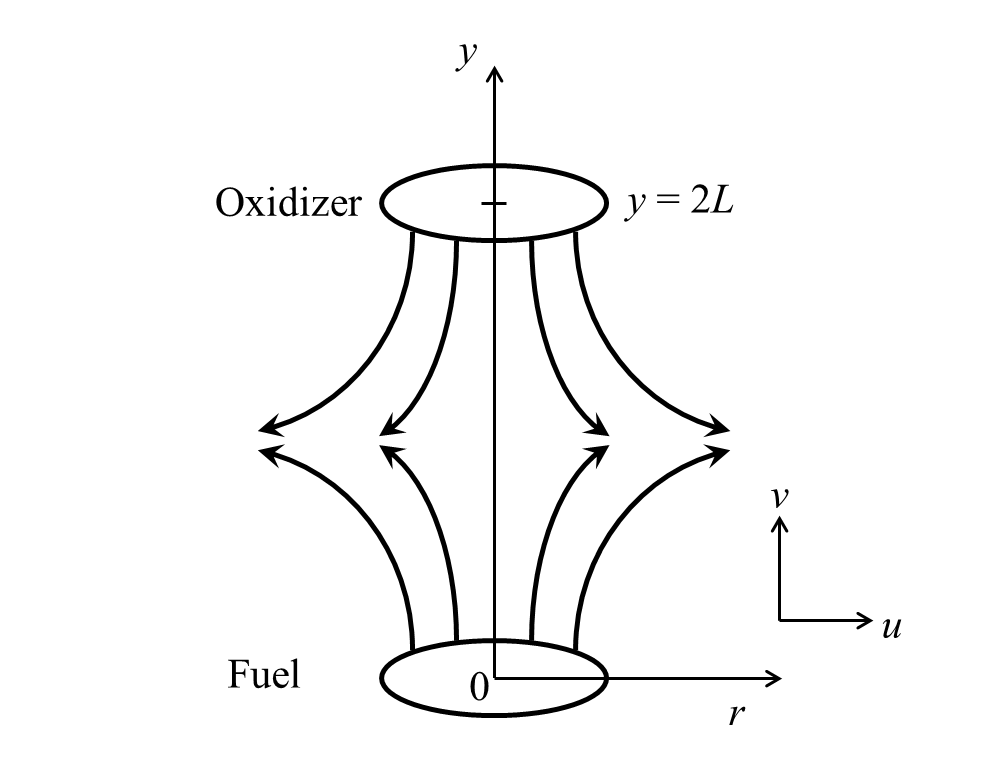
\includegraphics[width=0.8\textwidth]{ch-NTC/counterflow.png}
  \normalsize
  \caption{Schematic of the nonpremixed counterflow configuration for S-curve analysis.}
  \label{fig:CF}
\end{figure}

The governing equations for the counterflow nonpremixed flame are presented by Smooke and co-workers~\cite{giovangigli87,smooke88}.  In brief, the flow is assumed to be laminar, stagnation-point flow in cylindrical coordinates.  In practice, the infinite interval for potential flow is truncated and the boundary conditions are applied at $y = 0$ and $y = 2L$ for the fuel and oxidizer streams, respectively, where $L$ denotes the separation distance between the two nozzles.  The governing equations for mass, momentum, chemical species, and energy with boundary layer assumptions are considered, and the system is closed with the ideal gas law.  The free stream radial and axial velocities at the edge of the boundary layer (the fuel side boundary) are given by $u_{\rm e} = ar$ and $v_{\rm e} = -2ay$, where $a$ is the single strain rate throughout the flow.  Upon introducing the notation
\begin{equation}
f' = \frac{u}{u_{\rm e}},
\end{equation}    
\begin{equation}
V = \rho v,
\end{equation}
where $f'$ is related to the derivative of a modified stream function~\cite{dixon-lewis85}, $V$ is the axial mass flux, and $\rho$ is the gas density, the boundary layer equations can be transformed into a system of ordinary differential equations valid along the stagnation-point streamline $r=0$, summarized below.
\begin{equation}
\dd{V}{y} + 2a\rho f' = 0,
\end{equation}      
\begin{equation}
\dd{ }{y}\left(\mu \dd{f'}{y}\right) - V\dd{f'}{y} + a(\rho_{\rm e} - \rho (f')^2) = 0,
\end{equation}  
\begin{equation}
\dd{ }{y}\left(\rho Y_k V_k\right) + V\dd{Y_k}{y} - \dot{\omega_k}W_k = 0, k = 1,2,...,K,
\end{equation}  
\begin{equation}
\dd{ }{y}\left(\lambda \dd{T}{y} \right) - c_pV\dd{T}{y} - \sum_{k=1}^K \rho Y_k V_k c_{pk} \dd{T}{y} - \sum_{k=1}^K \dot{\omega_k}W_kh_k = 0.
\end{equation}  

In these equations, $\mu$, $\lambda$, and $c_p$ are the dynamic viscosity, heat conductivity, and the constant pressure heat capacity of the mixture, respectively.  For the $K$ species in total considered in the chemical mechanism, $Y_k$, $V_k$, $\dot{\omega_k}$, $W_k$, $c_{pk}$, and $h_k$ denote the mass fraction, diffusion velocity, molar production rate, molecular weight, constant pressure heat capacity, and specific enthalpy of each species, respectively.  

The numerical code adopted to solve them employs the damped Newton method and time integration solution scheme~\cite{smooke88}.  The S-curve marching is performed using the flame-controlling method of Nishioka \emph{et al.}~\cite{nishioka96} with detailed chemistry~\cite{kee89} and transport database~\cite{kee83}.

\section{Nonpremixed Cool Flames at Atmospheric Conditions}
\subsection{Identification of the Cool Flame} \label{sec:NTC-4.1}

Validation results for the experimental system are shown in Fig.~\ref{fig:M}.  Specifically, when the PMT captures the photons corresponding to the characteristic wavelength of CH$_2$O (peaks around $400$ nm), it outputs negative impulses to the oscilloscope, with the amplitudes of these impulses representing the light intensity.  Figure~\ref{fig:M} shows that such signal intensity drops after replacing either N$_2$-diluted DME with pure N$_2$ issued from the lower nozzle (at point a) or air with N$_2$ issued from the upper nozzle (at point c), demonstrating that the signal is due to the simultaneous presence of air and DME.  Since replacing air with the same flow rate of N$_2$ barely affects the temperature profile and the flow field, the signal difference between the air/DME and N$_2$/DME cases indicates the existence of NTC chemical activities.  It is noted that the signal from N$_2$/DME thermal pyrolysis is minimal, such that the difference in the chemically reactive and non-reactive cases can be completely attributed to the low-temperature oxidation chemistry.  

\begin{figure}[t]
  \centering
  \scriptsize
  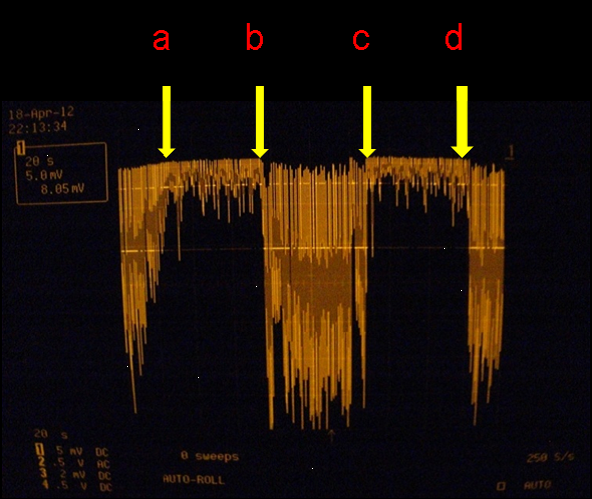
\includegraphics[width=0.7\textwidth]{ch-NTC/M.png}
  \normalsize
  \caption{``M'' shaped signal observed with the PMT-osillloscope system from the counterflow chamber at atmospheric pressure.  The fuel stream consists of 30\% DME and 70\% nitrogen, and the oxidizer is air.  a.~Switch Air/DME to Air/N$_2$; b.~Switch Air/N$_2$ to Air/DME; c.~Switch Air/DME to N$_2$/DME; d.~Switch N$_2$/DME to Air/DME.}
  \label{fig:M}
\end{figure}

In Fig.~\ref{fig:PMT}, the chemiluminescence intensity from the CH$_2$O under the strain rates of $40$, $60$, and $100$ /s were measured as a function of the air boundary temperature.  The time-averaged signal was acquired by the lock-in amplifier with an integration time of three seconds to minimize the noise, and the error bars show the standard deviation of the signals based on $1000$ samples. The results clearly show that the low-temperature chemistry becomes more pronounced at higher air temperatures and lower strain rates, with more CH$_2$O produced and therefore stronger chemiluminescence from it.

\begin{figure}[t]
  \centering
  \scriptsize
  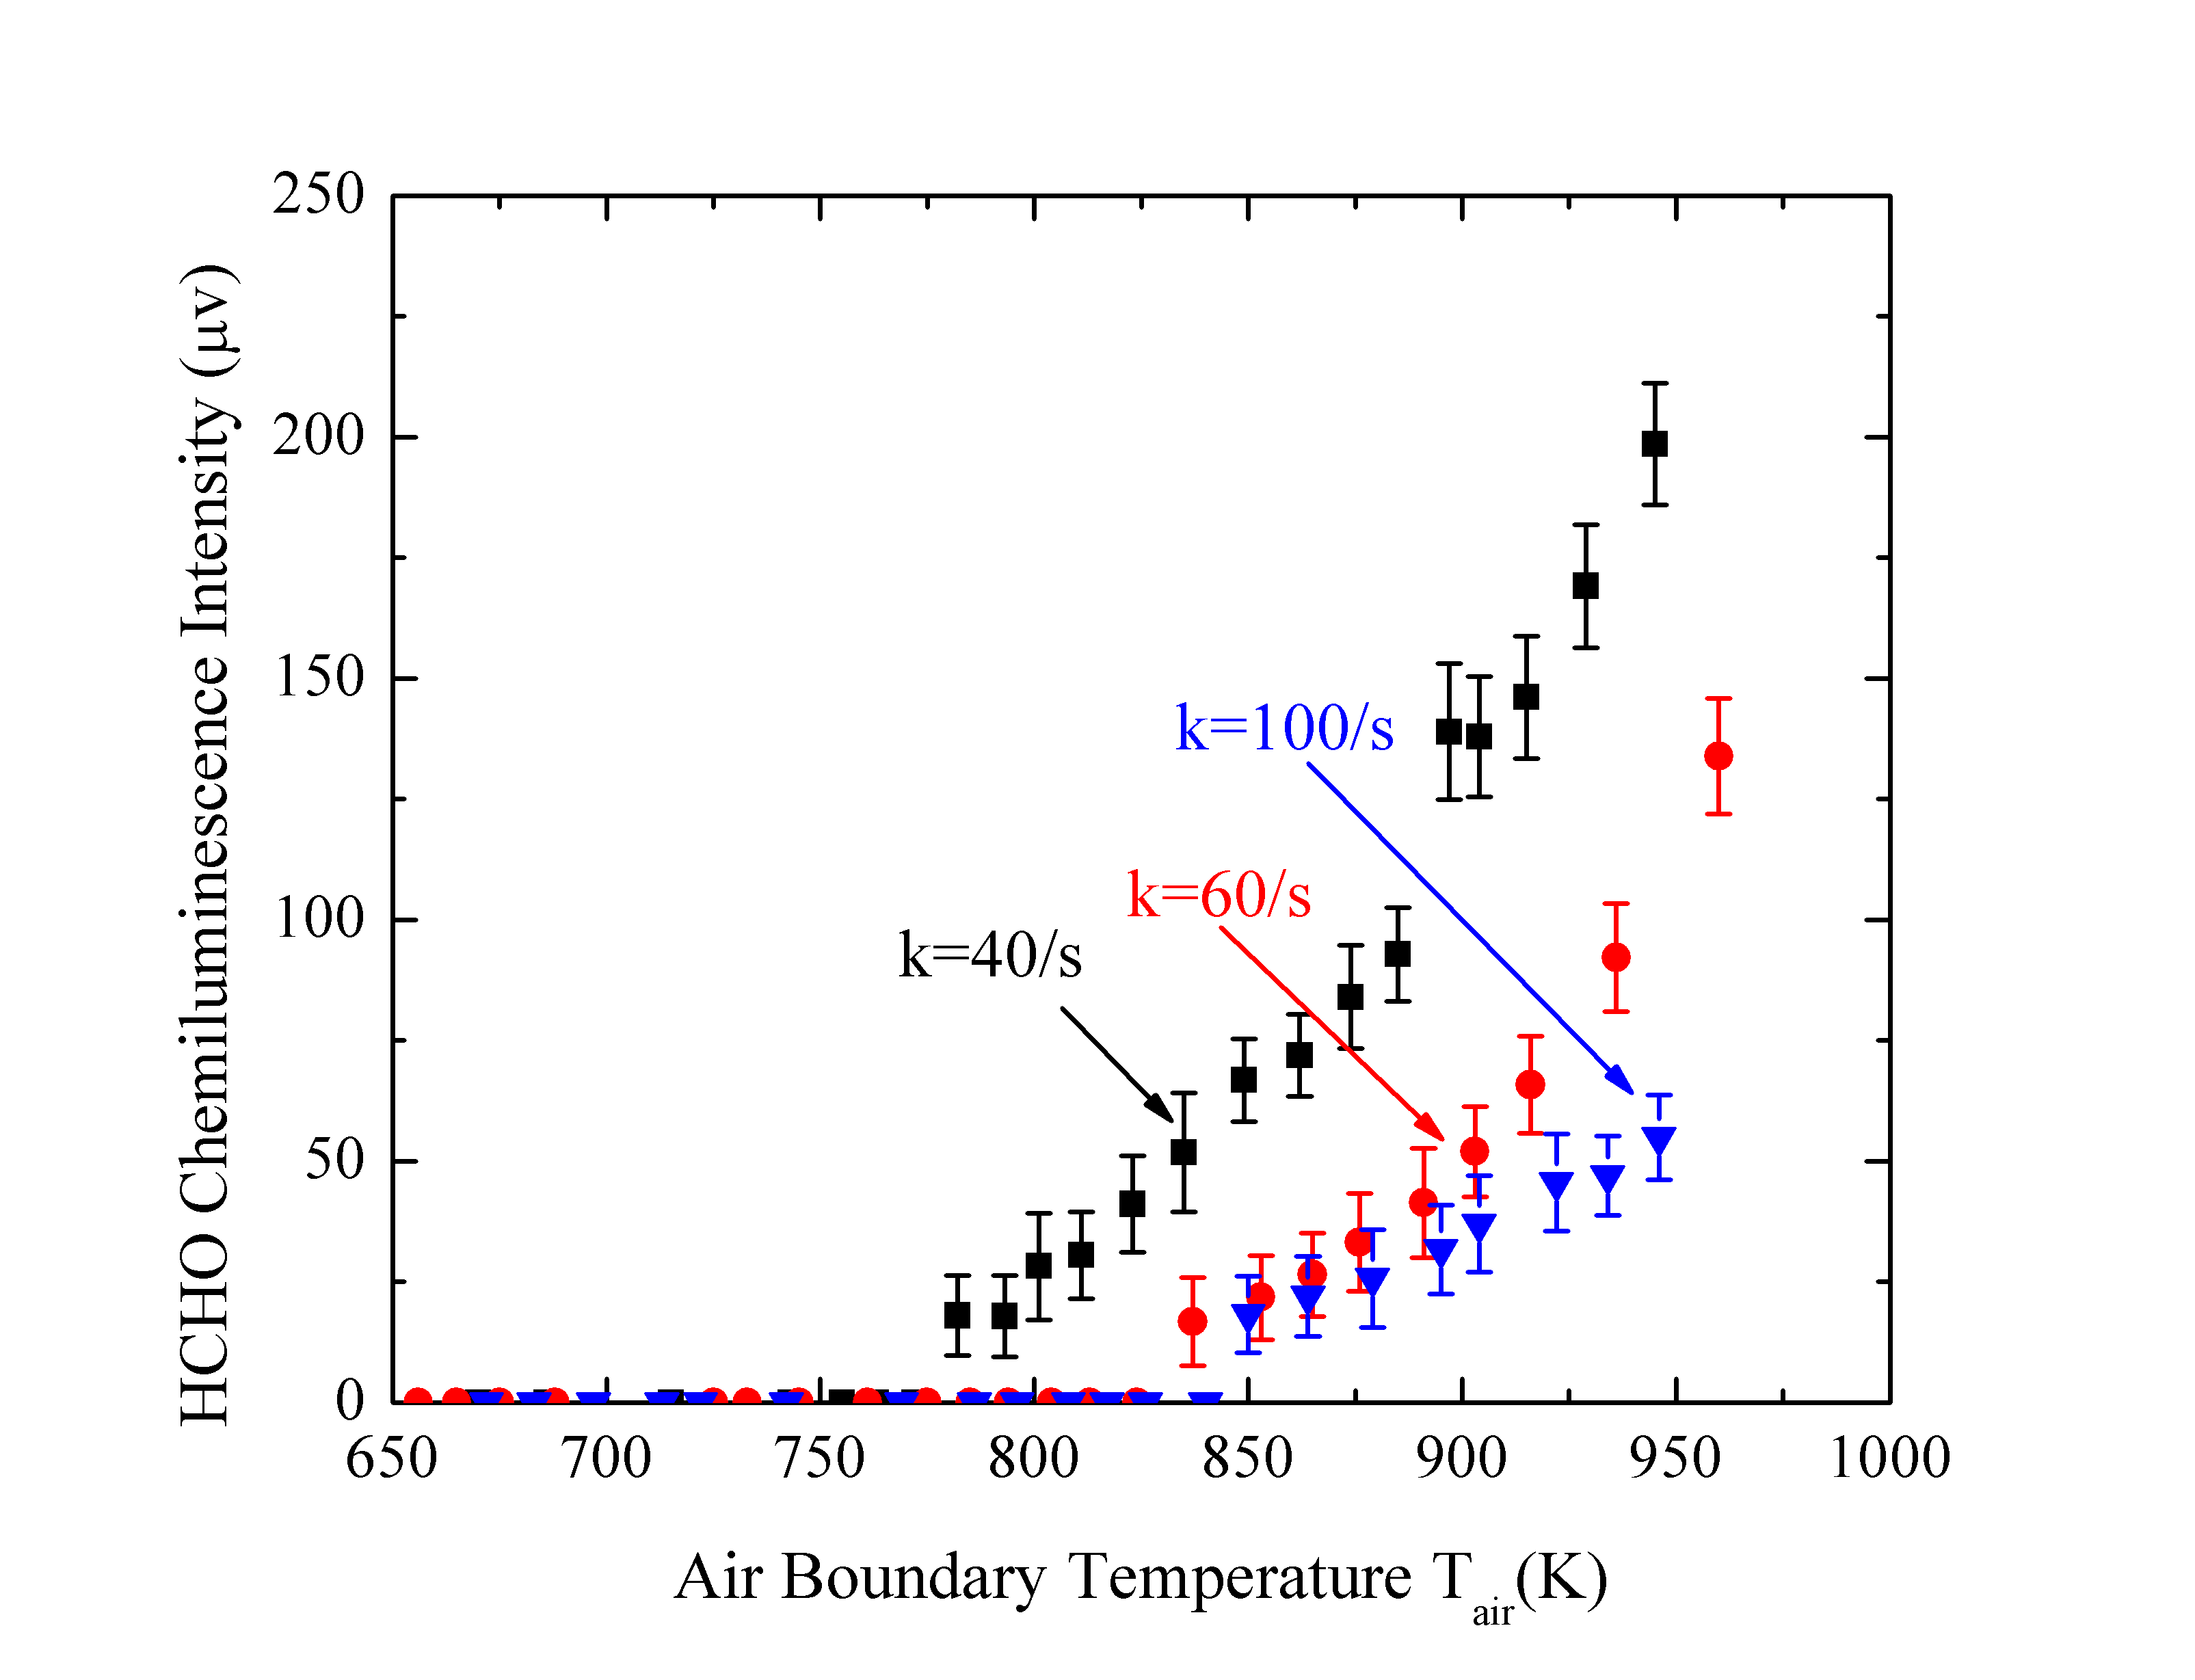
\includegraphics[width=1.0\textwidth]{ch-NTC/PMT.png}
  \normalsize
  \caption{Formaldehyde chemiluminescence intensity at different air boundary temperatures under various strain rates.}
  \label{fig:PMT}
\end{figure}

The above experimental observations are further corroborated by the calculated results of the maximum formaldehyde mole fraction versus the air temperature for $30\%$ DME in nitrogen, for different strain rates.  Figure~\ref{fig:Scurve-SR} shows the calculated secondary S-curve characterized by the low-temperature chemistry.  It is seen that the upper branch solution, designating the state of the low-temperature flame, shows the same experimental trend of increasing CH$_2$O concentration with increasing air temperature and decreasing strain rate.  The strongly transport-affected, nonpremixed counterflow have therefore been identified.  The fact that this chemical reactivity is localized in a thin “flame” region is demonstrated in the next section.

\begin{figure}[t]
  \centering
  \scriptsize
  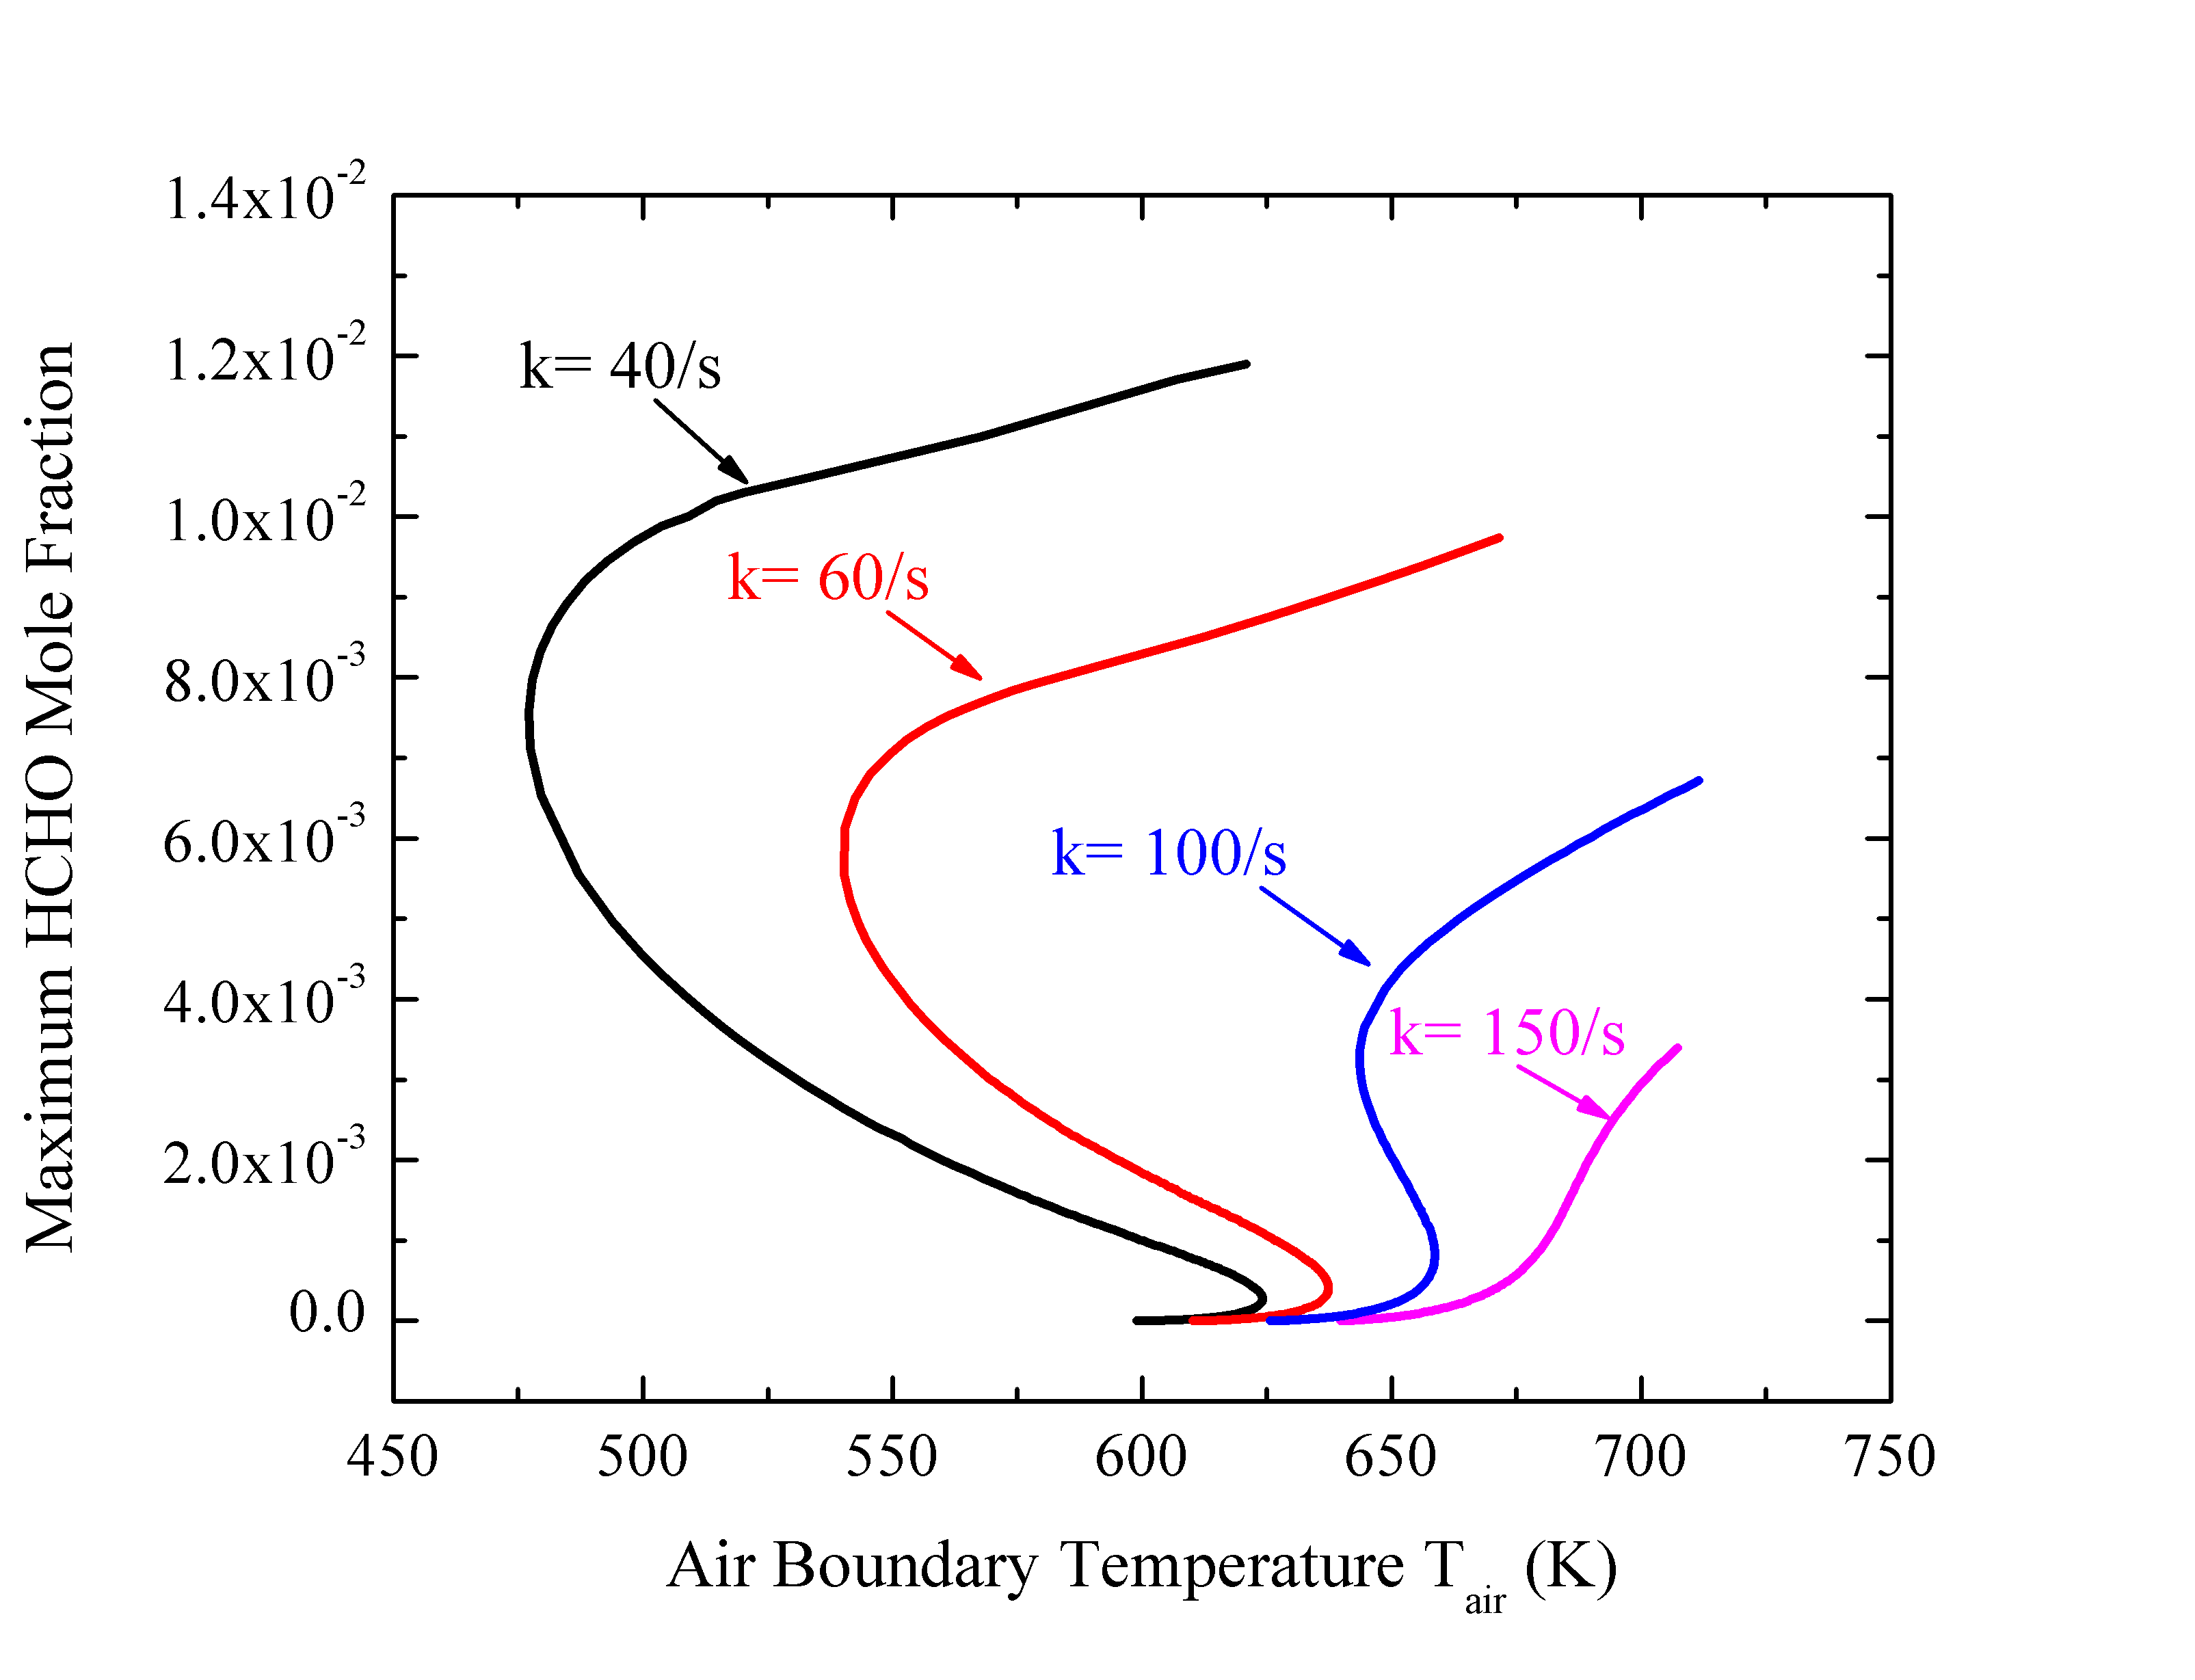
\includegraphics[width=1.0\textwidth]{ch-NTC/Scurve-SR.png}
  \normalsize
  \caption{Maximum formaldehyde mole fraction of $30\%$ DME at different air boundary temperatures under various strain rates.}
  \label{fig:Scurve-SR}
\end{figure}

\subsection{Determination of Ignition Temperature} \label{sec:NTC-4.2}

\begin{figure}[ht]
  \centering
  \scriptsize
  \vspace{0.3in}
  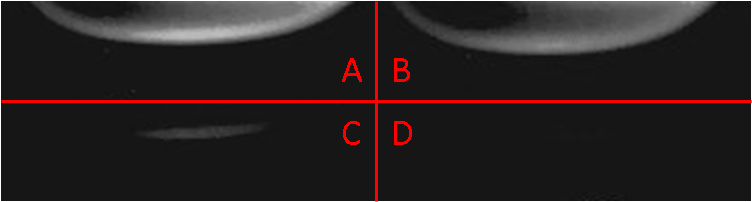
\includegraphics[width=0.8\textwidth]{ch-NTC/IR.png}
  \normalsize
  \caption{A/B: Heated air/N$_2$ against DME counterflow IR images at ignition (atmospheric pressure, strain rate $60$ /s); C/D: Difference between A/B and B.}
  \label{fig:IR}
\end{figure}

Detections of the state of ignition of the NTC-flame are therefore proceeded, as identified by the lower turning points in Fig.~\ref{fig:Scurve-SR}.  Since the chemiluminescence intensity from the above experimentation is not strong enough to detect the low level of CH$_2$O concentration at ignition, detections of ignitions have been resorted to capturing the infrared radiation from the ignition process by using a highly sensitive infrared camera, FLIR SC640 (with the thermal sensitivity about $60$ mK at $303$ K), as shown on the right part of Fig.~\ref{fig:NTC-setup}.  The brightness of the IR images in Fig.~\ref{fig:IR} indicates the IR radiation intensity, with the bright color denoting higher radiation intensity than the dark color.  Since both the air/DME and N$_2$/DME flows now radiate infrared signals when heated due to the excitation of the vibrational modes of the gas molecules in the thermal mixing layer, the “background” N$_2$/DME signal needs to be subtracted out from the air/DME signal to isolate/identify the emission due to the low-temperature chemical reactivity.  Consequently, by gradually increasing the air boundary temperature, and by setting the IR radiation intensity of the N$_2$/DME flow as the reference state, the first appearance of an excess signal from the air/DME flow would indicate the onset of ignition.  In practice, when the air boundary temperature reaches the regime of interest, only $1$ K is increased each time at the air boundary before the flow becomes steady again.  It is fairly clear that at a certain temperature, which is defined as the ignition point, the signal from air/DME starts to exceed that of the reference state.  Such temperature measurements are repeatable within $\pm 2$ K.  A typical result is shown in Fig.~\ref{fig:IR}, in which the A and B panels are the raw IR signals for heated air and N$_2$ against DME, which are respectively reactive and nonreactive.  Panels C and D respectively show the residue signals of panels A and B after the background signal from panel B is subtracted; the null signal for D is obtained by default.  The temperature at which a discernable image of radiation is detected is then identified as that of ignition, as is the case for panels A/C, for the corresponding strain rate.

The localized nature of the IR radiation, shown in panel C, then also supports the notion that the chemical reactivity observed herein has the characteristic of a flame, in support of the interpretation of the chemiluminescence signal reported in the previous section.

\begin{figure}[t]
  \centering
  \scriptsize
  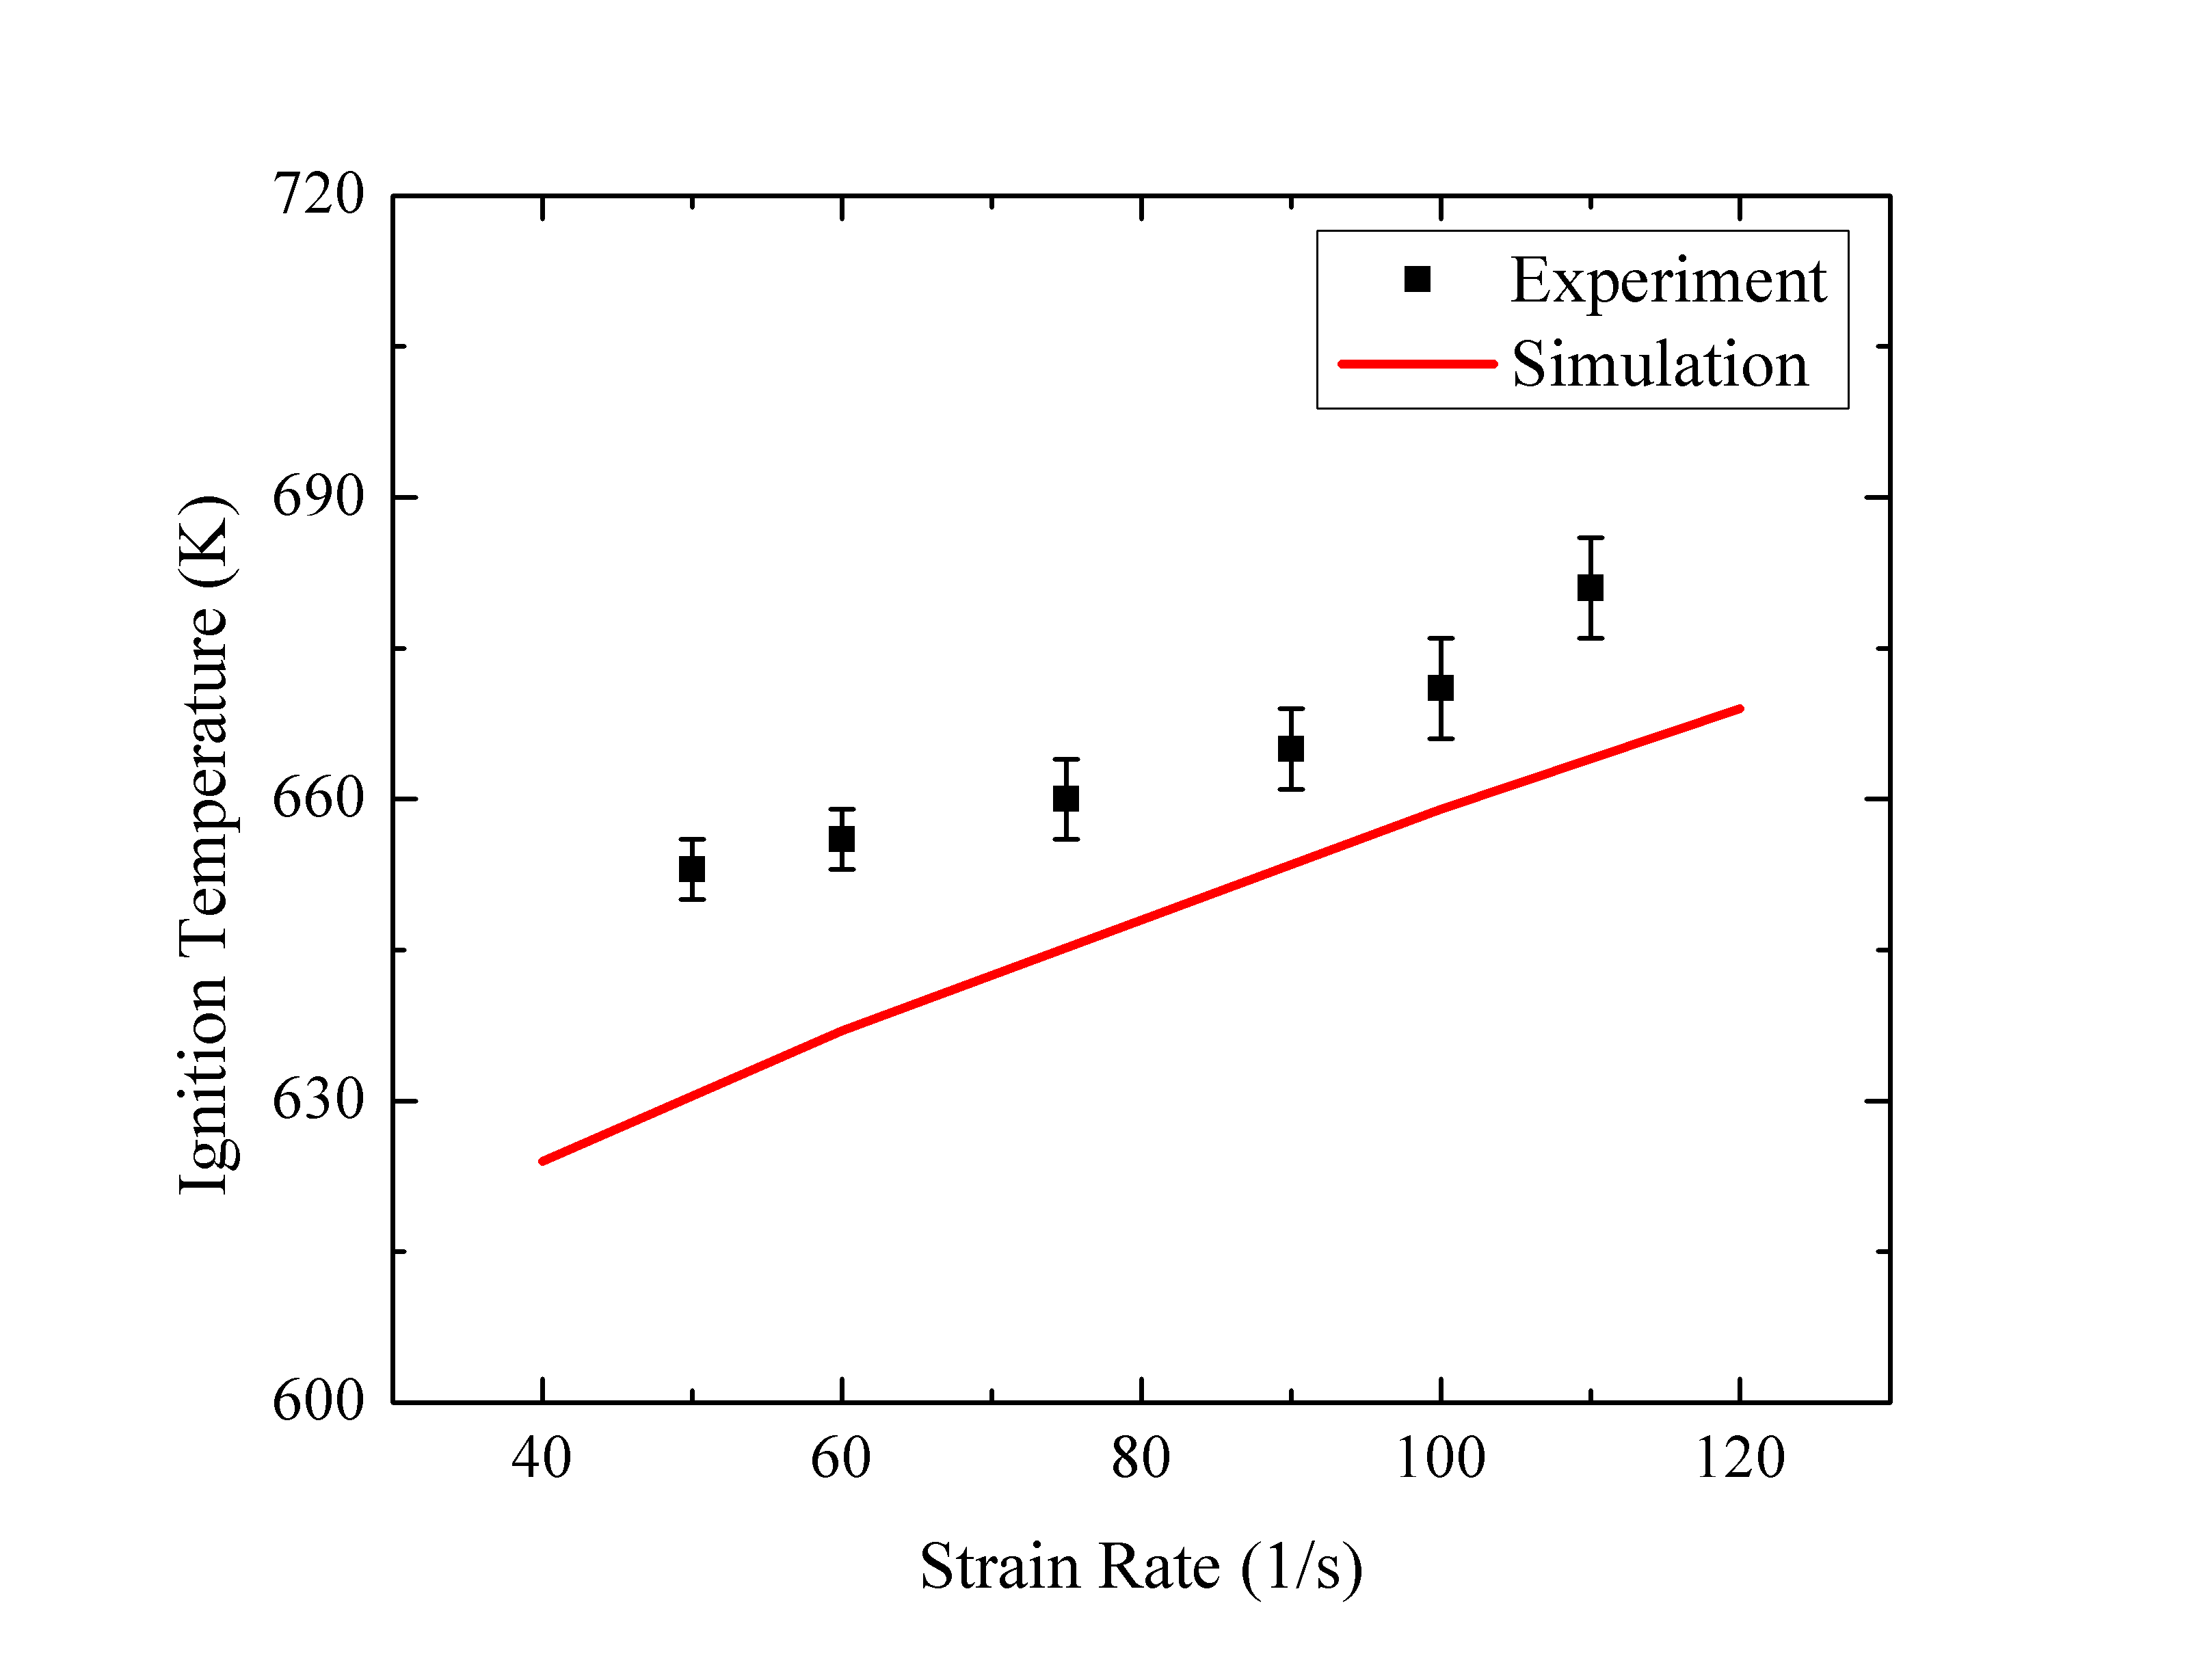
\includegraphics[width=1.0\textwidth]{ch-NTC/Ign-SR.png}
  \normalsize
  \caption{Calculated and observed ignition temperatures of $30\%$ DME under various strain rates at atmospheric pressure.}
  \label{fig:Ign-SR}
\end{figure} 

\begin{figure}[t]
  \centering
  \scriptsize
  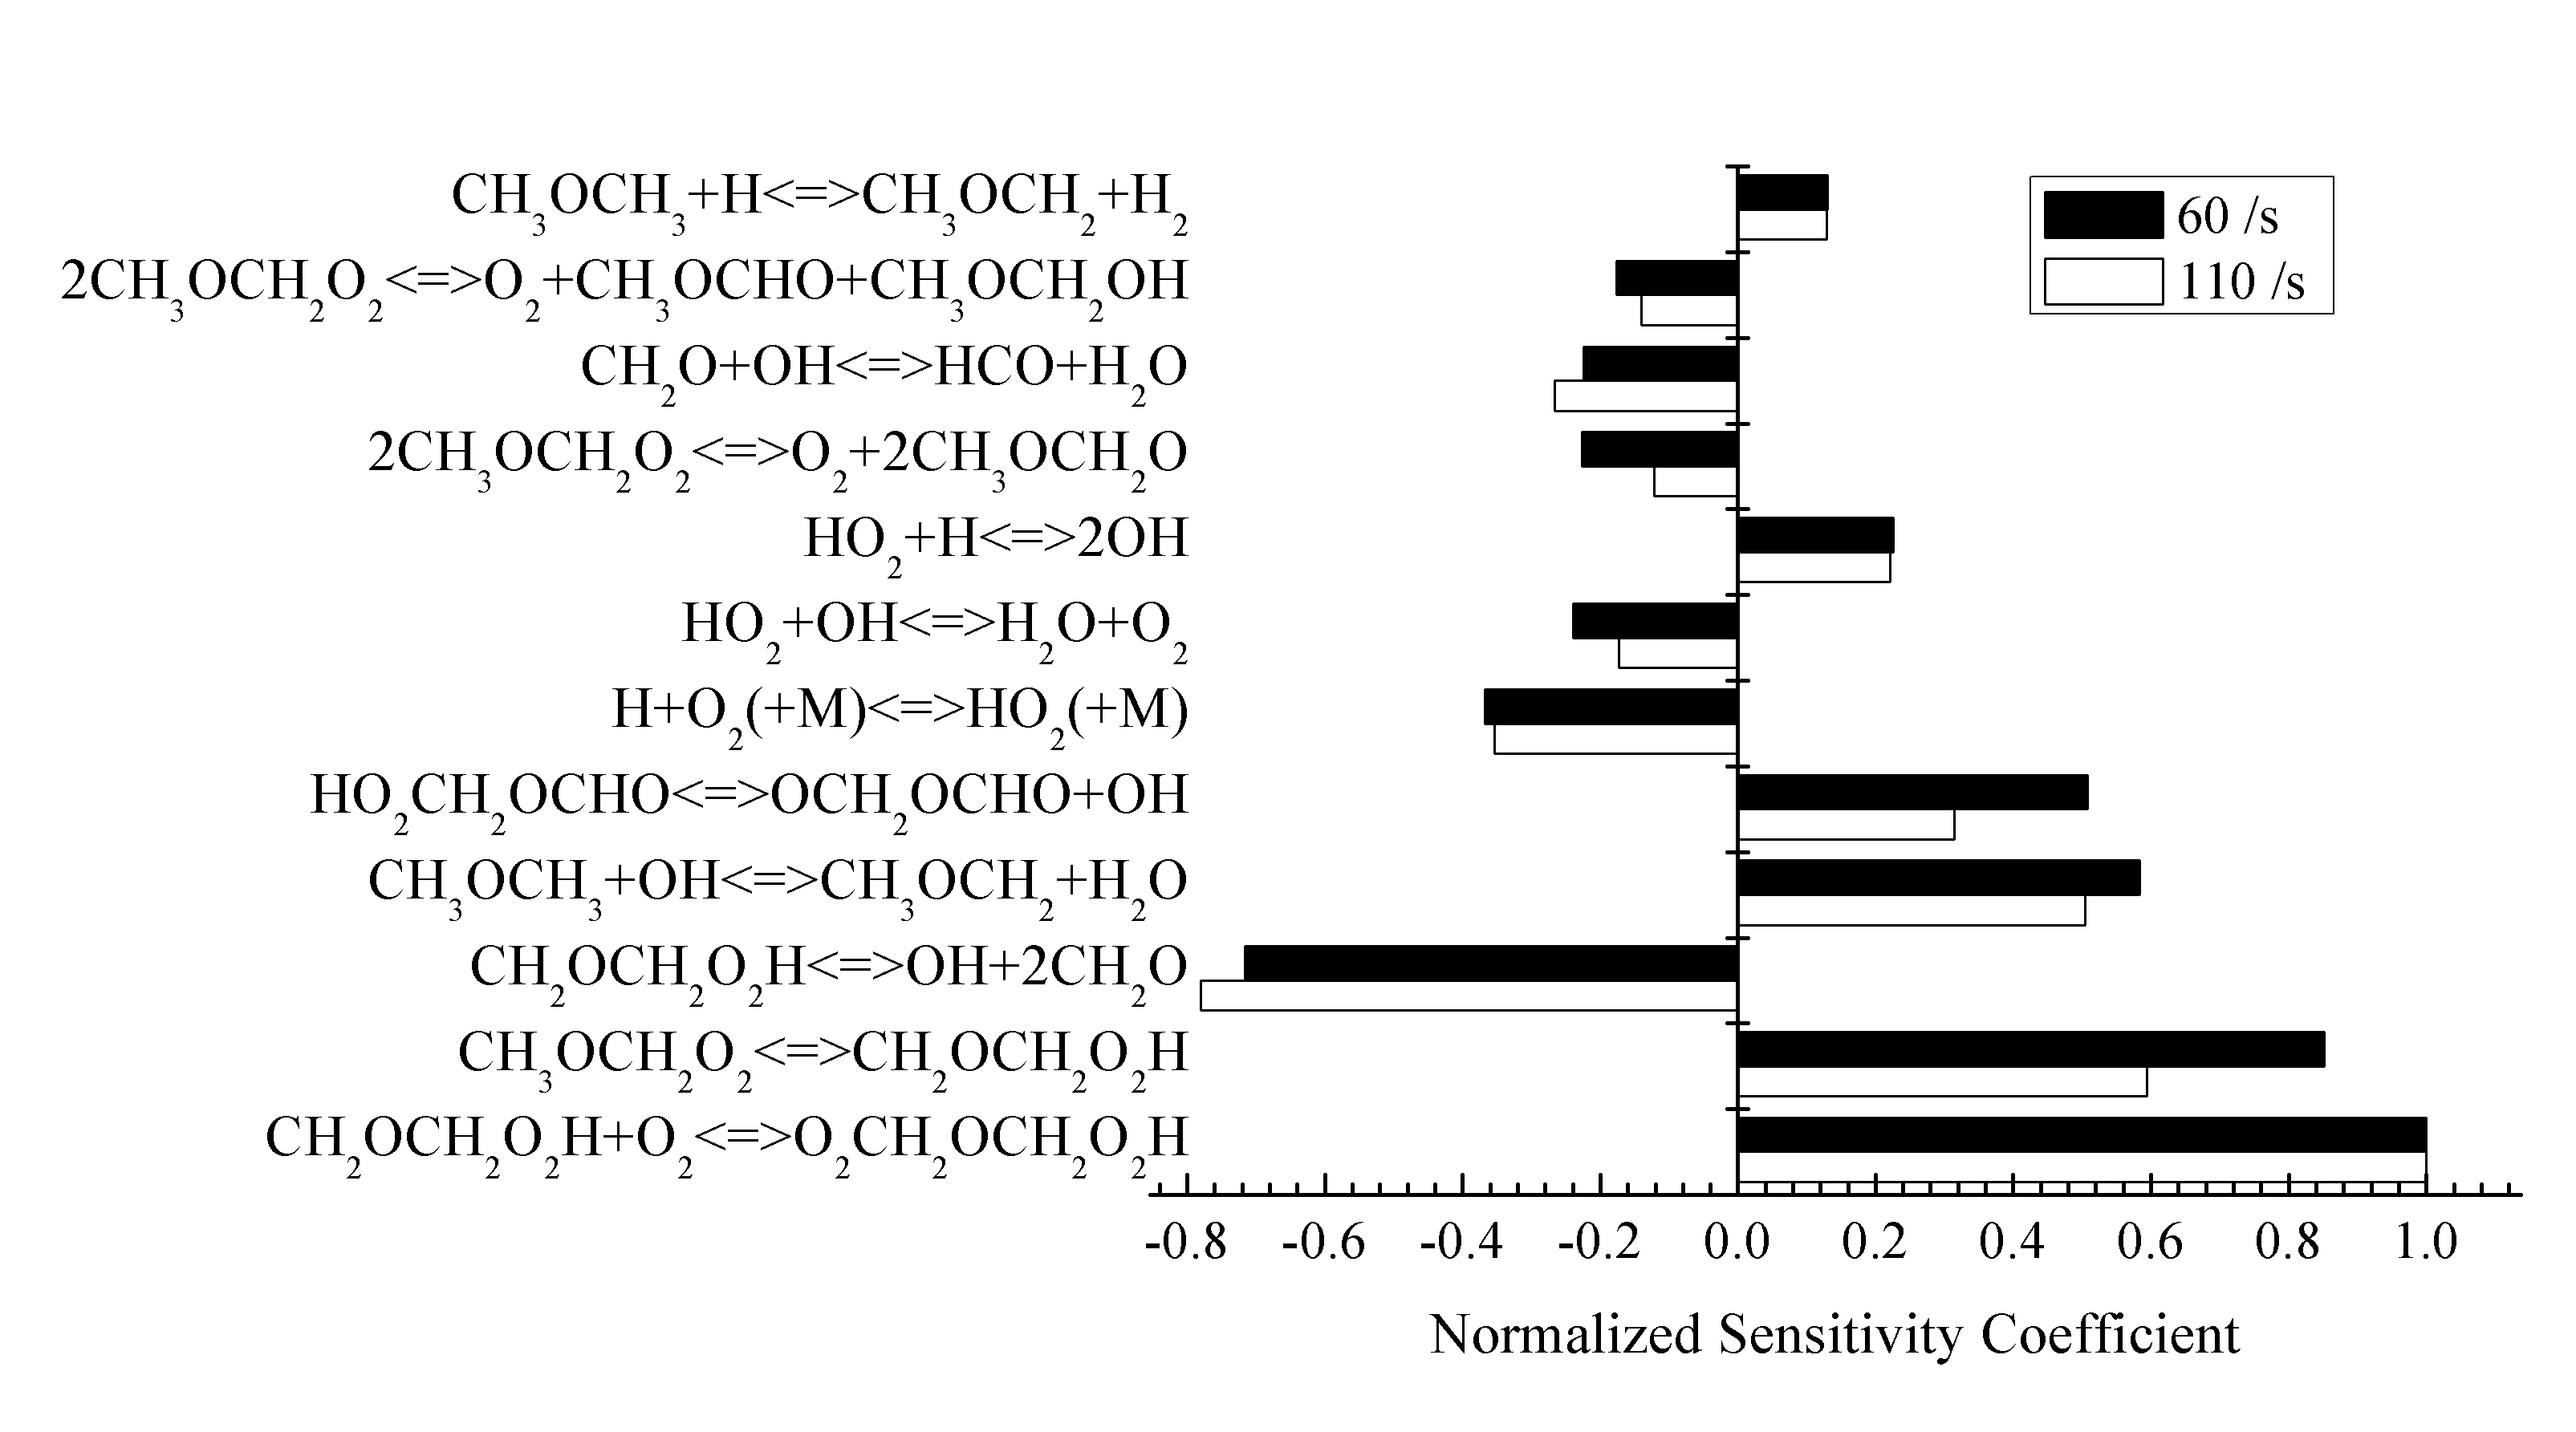
\includegraphics[width=1.0\textwidth]{ch-NTC/Sen_SR.png}
  \normalsize
  \caption{Sensitivity analysis on low and high strain rate cases at atmospheric pressure: DME mole fraction is $30\%$.}
  \label{fig:Sen_SR}
\end{figure}

Figure~\ref{fig:Ign-SR} shows the IR measurements of the low-temperature chemistry induced ignition, as determined through the above procedure, as a function of the strain rate.  The uncertainty bars account for those from the thermocouple radiation correction as well as reproducibility of the experimental measurements.  Due to the moderate flow field temperatures and the high sensitivity of the thermocouple, the uncertainty bars of the ignition temperatures are quite small.  These experimental values are then compared with those corresponding to the calculated lower, ignition turning points.  Figure~\ref{fig:Ign-SR} shows satisfactory agreement, with the average temperature difference being within $20$ K.

Sensitivity analysis was further performed for the state of ignition, as shown in Fig.~\ref{fig:Sen_SR}.  It is seen that the controlling chemistry is indeed the low tempearature chemistry, corresponding to the first stage ignition of the homogeneous autoignition process in the NTC-affect regime.  More specifically, the first two most important reactions that promote the low-temperature chemistry induced ignition are the oxygen combination reaction CH$_2$OCH$_2$O$_2$H+O$_2$ $\Leftrightarrow$ O$_2$CH$_2$OCH$_2$O$_2$H and the isomerization reaction CH$_3$OCH$_2$O$_2$ $\Leftrightarrow$ CH$_2$OCH$_2$O$_2$H, while the most important retarding reaction is the $\beta$-scission reaction CH$_2$OCH$_2$O$_2$H $\Leftrightarrow$ OH+$2$CH$_2$O.  These two groups of reactions compete for the CH$_2$OCH$_2$O$_2$H radicals and as such function oppositely.

\begin{figure}[t]
  \centering
  \scriptsize
  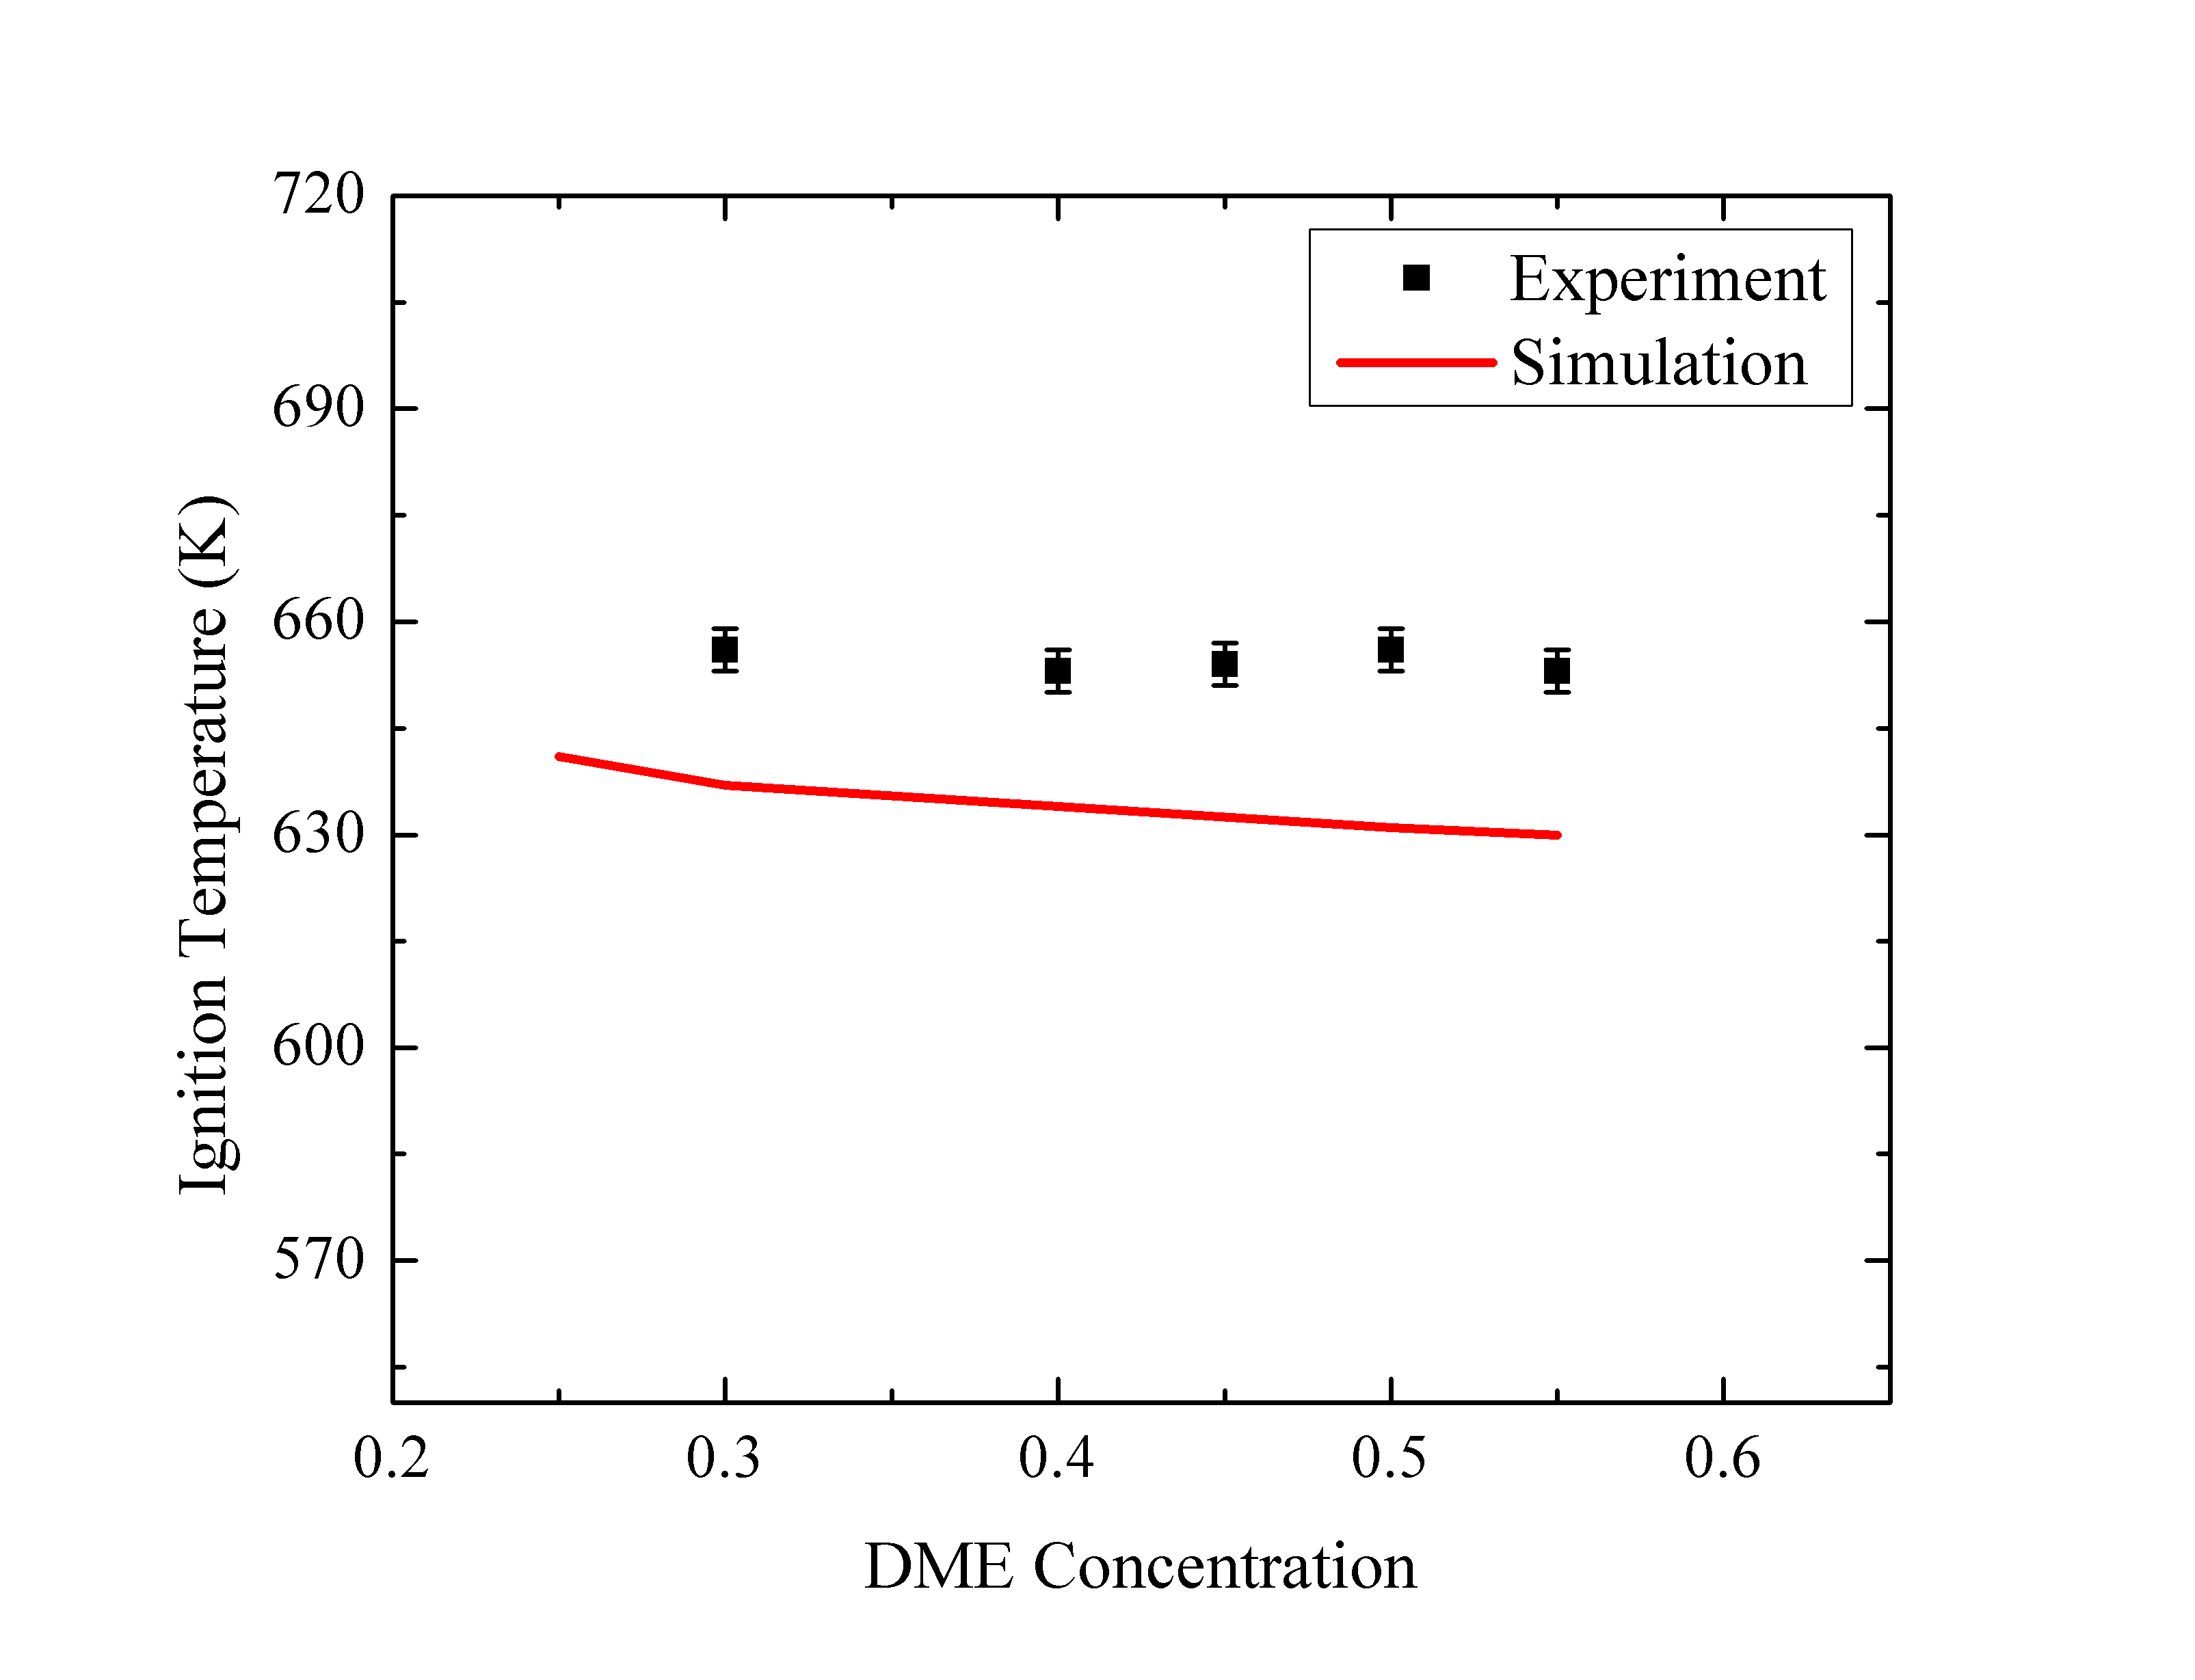
\includegraphics[width=1.0\textwidth]{ch-NTC/Ign-Con.png}
  \normalsize
  \caption{Ignition temperatures of various DME concentrations under the strain rate of $60$ /s at atmospheric pressure.}
  \label{fig:Ign-Con}
\end{figure}

In addition to the effects of strain rate on the ignition temperature, the effects of DME concentration have also been evaluated, shown, and compared with the simulation results in Fig.~\ref{fig:Ign-Con}.  The simulation result basically demonstrates the insensitive nature of the NTC-affected ignition temperature to the variation of the boundary DME concentrations over an extensive range of DME concentrations, under a fixed strain rate of $60$ /s.  The experimental results again show good agreement with the simulation results.  This effect corresponds to the insensitive nature of the equivalence ratio in the low-temperature chemistry, given the fact that the first-stage delay is insensitive to the equivalence ratio in the homogeneous autoignition process~\cite{zhao13}.  Sensitivity analysis corresponding to different boundary DME concentrations were also carried out, showing the same controlling chemistry as that of Fig.~\ref{fig:Sen_SR}.

\section{Nonpremixed Cool Flames at Elevated Pressure}

Recognizing that low-temperature chemistry is more pronounced at elevated pressure, which for example could affect flame stabilization, as will be shown in Chapter~\ref{ch:dynamics}, a systematic experimental and computational study on nonpremixed DME cool flames at elevated pressures is presented here.  Although the experimental approach presented in Sec.~\ref{sec:NTC-4.1} is able to capture the ignition temperature of nonpremixed cool flame, it has two major limitations.  First, the infrared signal is not able to penetrate the quartz window of the counterflow chamber for elevated pressure experiments.  Second, due to the experimental procedure of switching between the oxidizer and inert for ignition detection, the extinction temperature of the nonpremixed cool flame cannot be measured.  Therefore, the experimental system and the detection method for cool flame ignition and extinction need to be improved.

\subsection{Improvement of the Experimental Methodology}

The counterflow system is kept the same as described in Sec.~\ref{sec:NTC-exp}.  To accommodate experiments at elevated pressures, the exhaust valve of the chamber is adjusted to balance the inflow and outflow and maintain the desired chamber pressure.

The major improvement here is the cool flame detection method.  A high-sensitivity monochrome CCD camera with high relative response in the UV spectrum (CCE-B013-U) was used to capture the global chemiluminescence from the low-temperature chemical reactions, which indicated the intensity of the cool flame similar to Zhao \emph{et al.}~\cite{zhao16}.  The exposure time of the UV camera is the same 6 seconds for all cases.  The ignition/extinction states of the cool flame were determined by gradually changing the oxidizer boundary temperature for a given fuel/oxidizer flow rate, until the chemiluminescence signal of the cool flame respectively emerged/disappeared as detected by the camera.  The ignition and extinction temperatures were quantified with the corresponding oxidizer boundary temperatures measured with an uncoated K-type (Chromel-Alumel) thermocouple after radiation correction as in Sec.~\ref{sec:NTC-exp}.

In the following discussion, a fuel stream consisting of 50\% DME and 50\% nitrogen at room temperature was issued from the lower nozzle and impinged onto the heated oxidizer stream from the upper nozzle.  The oxygen volume fraction in the oxidizer stream varied from 21\% to 25\%, and the 
ambient pressure varied from 2 to 3 atm for ignition and extinction measurements.  The global strain rate used in the following discussion is defined as the pressure-weighted gradient of the axial flow velocity~\cite{seiser00}.  The experimental affirmation of the distinctive ignition and extinction behavior of nonpremixed cool flame is first demonstrated to validate the computational prediction.  Then, the thermal and chemical structures of the reacting layer in the counterflow system at cool flame ignition, steady cool flame, and cool flame extinction conditions are analyzed, elucidating the dominant chemical pathways for each condition.   Possible reasons for the discrepancies between experiments and computations are discussed.  Finally, the effects of ambient pressure and oxygen concentration on ignition and extinction are discussed.  

\subsection{Hysteretic Ignition and Extinction Behavior}

What differentiates a strained cool flame from a reacting mixture going through slow oxidation in a heated flow is the hysteretic ignition and extinction behavior.  Such hysteretic behavior has already been illustrated with an S-curve analysis shown in Fig.~\ref{fig:Scurve-SR} but is further explained in Fig.~\ref{fig:Scurve-hys}.  The numerical code and chemical model adopted here are the same as in Sec.~\ref{sec:NTC-comp}.  \emph{A posteriori} analysis based on the optically thin radiation model, with radiative properties based on the RADCAL model by Grosshandler of NIST~\cite{grosshandler93} shows that the radiative heat loss is minimal, and therefore radiation is not included in the current computation.  At a fixed strain rate, by gradually increasing the air boundary temperature and hence the reactivity and heat generation rate within the flow, at some point within the flow the temperature will exceed the boundary temperature and eventually lead to self-sustained burning.  Such a transition state I is defined as the ignition point, and the condition after ignition that is located on the upper steady branch of the S-curve is designated as point S, representing a steady cool flame.  The difference in the maximum temperatures between points S and I primarily results from the heat release from the cool flame.  As this temperature decreases from point S, the maximum temperature in the flow field also decreases, following the upper branch trajectory, until the flame extinguishes at point E.  The difference in the air boundary temperature between points I (or S) and E demonstrates the hysteresis between the ignition and extinction of the flame. 

\begin{figure}[t]
  \centering
  \scriptsize
  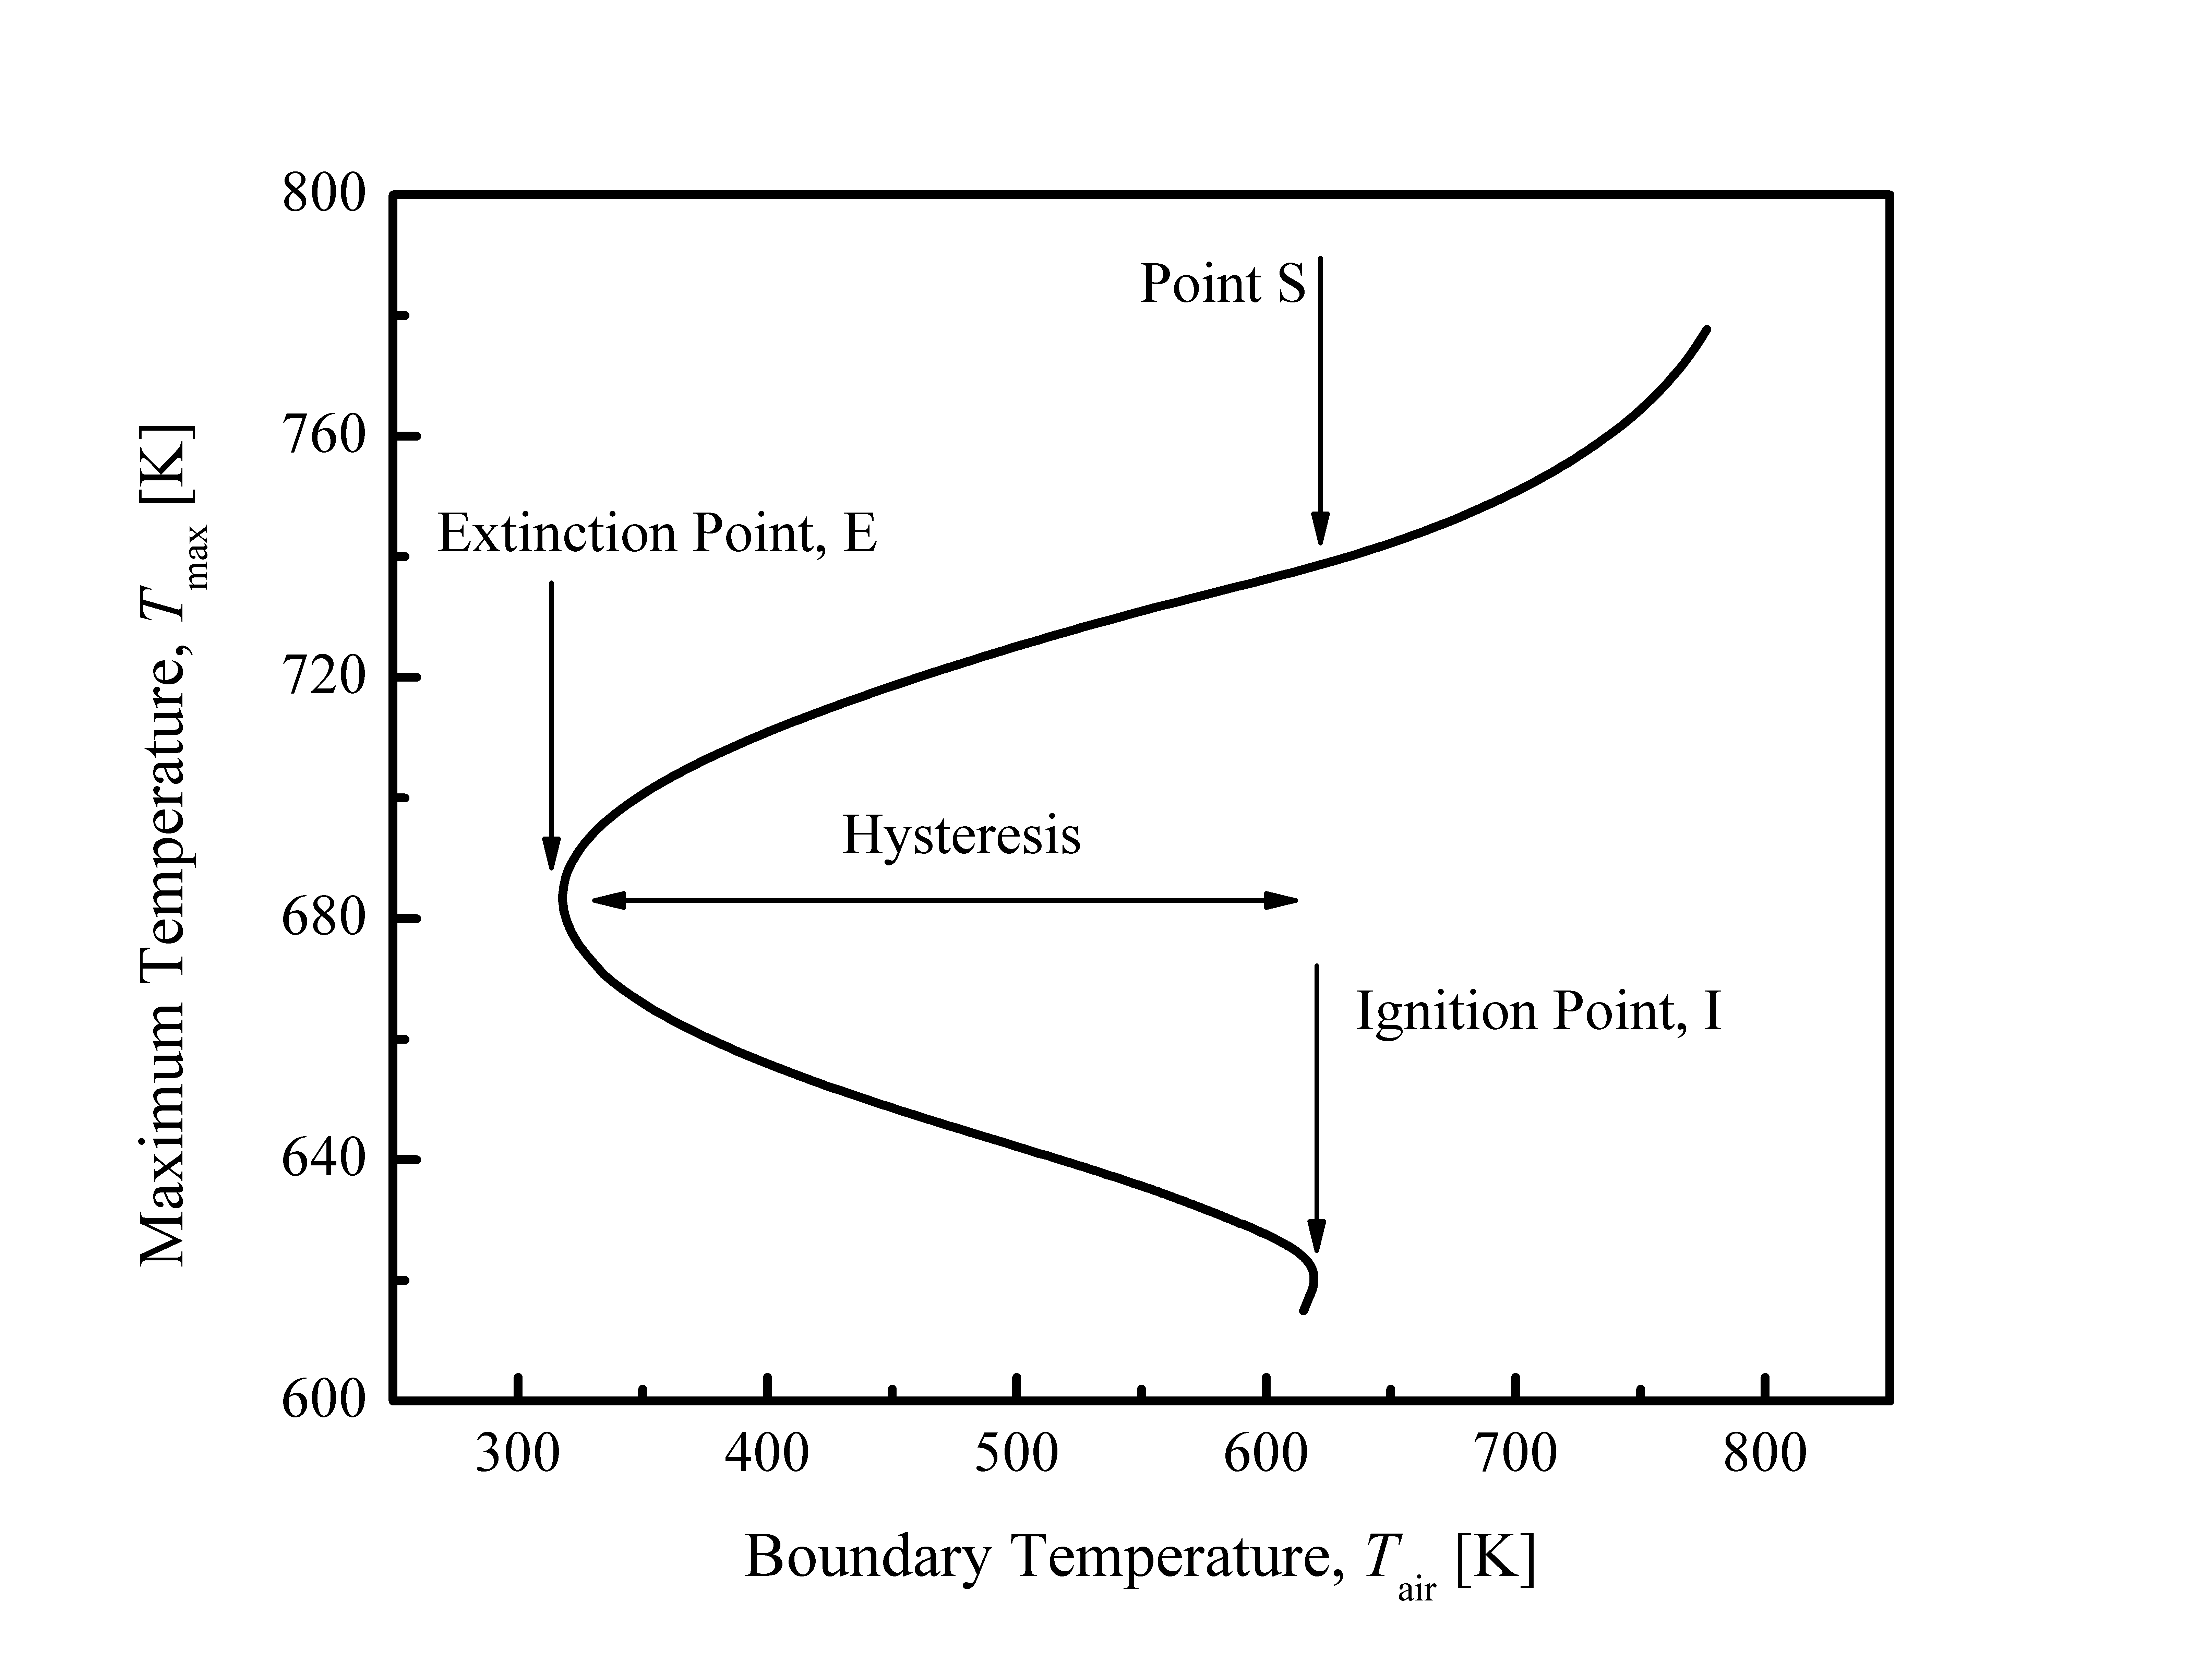
\includegraphics[width=1.0\textwidth]{ch-NTC/S-Curve.png}
  \normalsize
  \caption{S-curve analysis of the response of nonpremixed counterflow of 50\% DME and 50\% nitrogen versus heated air at the 2 atm and pressure-weighted strain rate of 80 /s.}
  \label{fig:Scurve-hys}
\end{figure}

To capture this computationally predicted hysteresis, the ignition and extinction temperatures were experimentally measured in the counterflow configuration based on the chemiluminescence of the cool flame.  Figure~\ref{fig:UV} shows representative images of the ignition and extinction detection for the DME/air cool flame at 2 atm and pressure-weighted strain rate of 84 /s.  Ignition of the cool flame is achieved by gradually increasing the oxidizer boundary temperature.  As shown in the left column of Fig.~\ref{fig:UV}, when the oxidizer boundary temperature is slowly increased from 626 K to 637 K (A to D), the chemiluminescence from the low-temperature chemistry suddenly becomes detectable by the UV camera, indicating onset of the cool flame.  The oxidizer boundary temperature is then gradually reduced with a temperature interval of 1 K, while maintaining quasi-steadiness at each step.  The right column of Fig.~\ref{fig:UV} then shows that, while the cool flame chemiluminescence remains as the boundary temperature is decreased from 637 K to 626 K (E to H), it suddenly vanishes at 626 K, which was thus defined as the extinction temperature.

\begin{figure}[t]
  \centering
  \scriptsize
  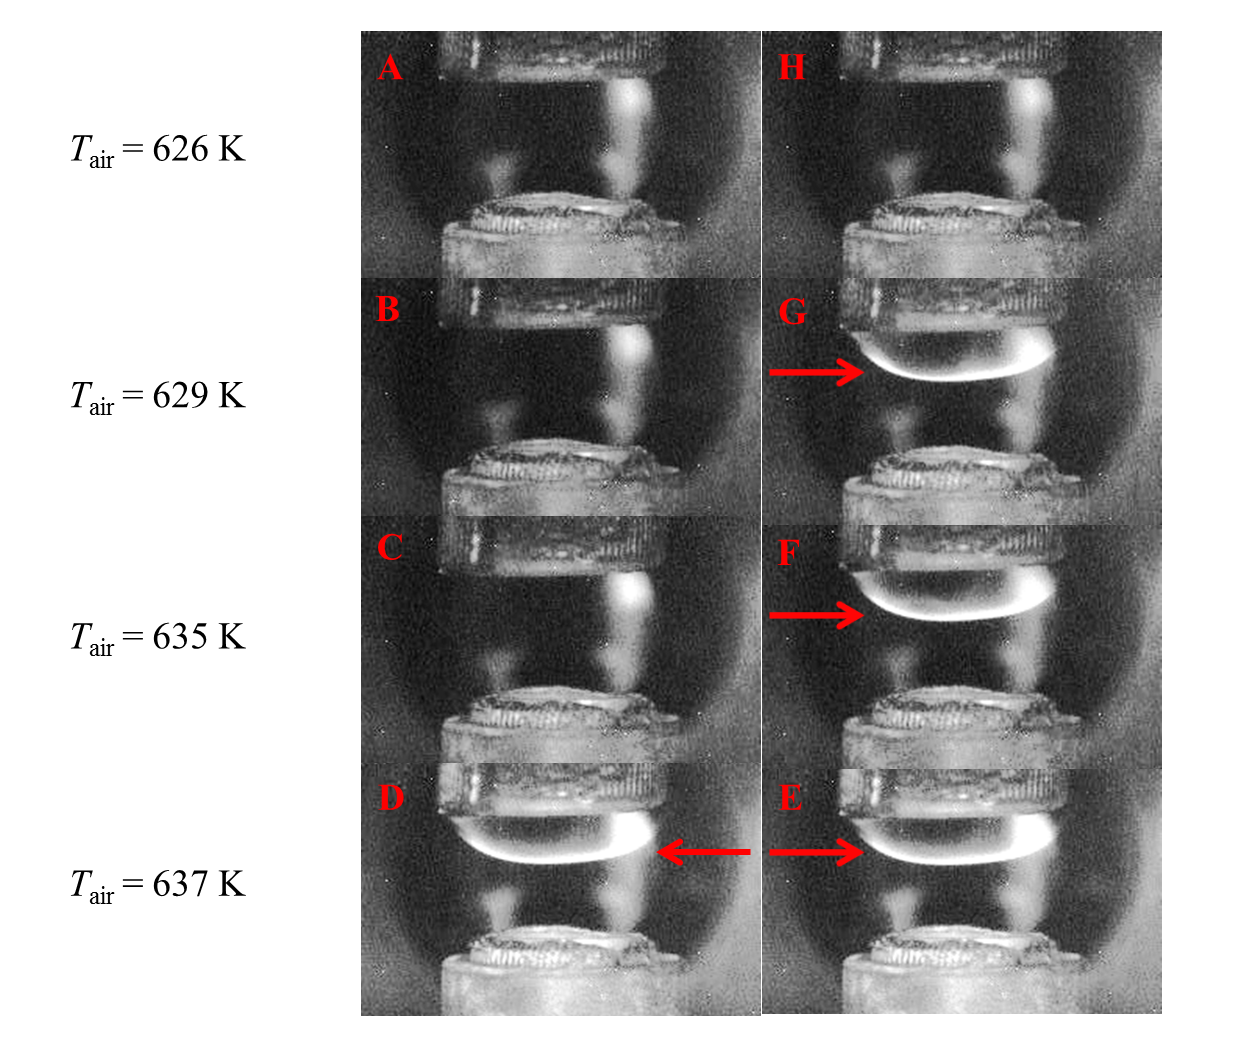
\includegraphics[width=1.0\textwidth]{ch-NTC/UV.png}
  \normalsize
  \caption{Flame images demonstrating the hysteretic nature of ignition and extinction of cool flames with air temperature. DME cool flame at 2 atm and pressure-weighted strain rate of 84 /s; DME volume fraction in the fuel stream is 50\%, and the oxidizer stream is air.}
  \label{fig:UV}
\end{figure}

The same procedure was followed to obtain the ignition and extinction temperatures at various strain rates for comparisons with the computationally predicted values, as shown in Fig.~\ref{fig:cmp_demo}.  Results from experiment and computation then both show that the ignition and extinction temperatures increase with increasing strain rate, due to reduced residence time.  Furthermore, the ignition temperature not only is higher than the extinction temperature at a given strain rate, it is also less sensitive to the strain rate, resulting in a less pronounced ignition-extinction hysteresis. Noting that the repeatability of the measurement is within 2 K, which is within the marker size in the figure, and the error bar represents the uncertainty of the radiation correction using different models, comparison between the experimental data should be made based on the upper or lower bound of the uncertainty bar across all the measurements.

\begin{figure}[t]
  \centering
  \scriptsize
  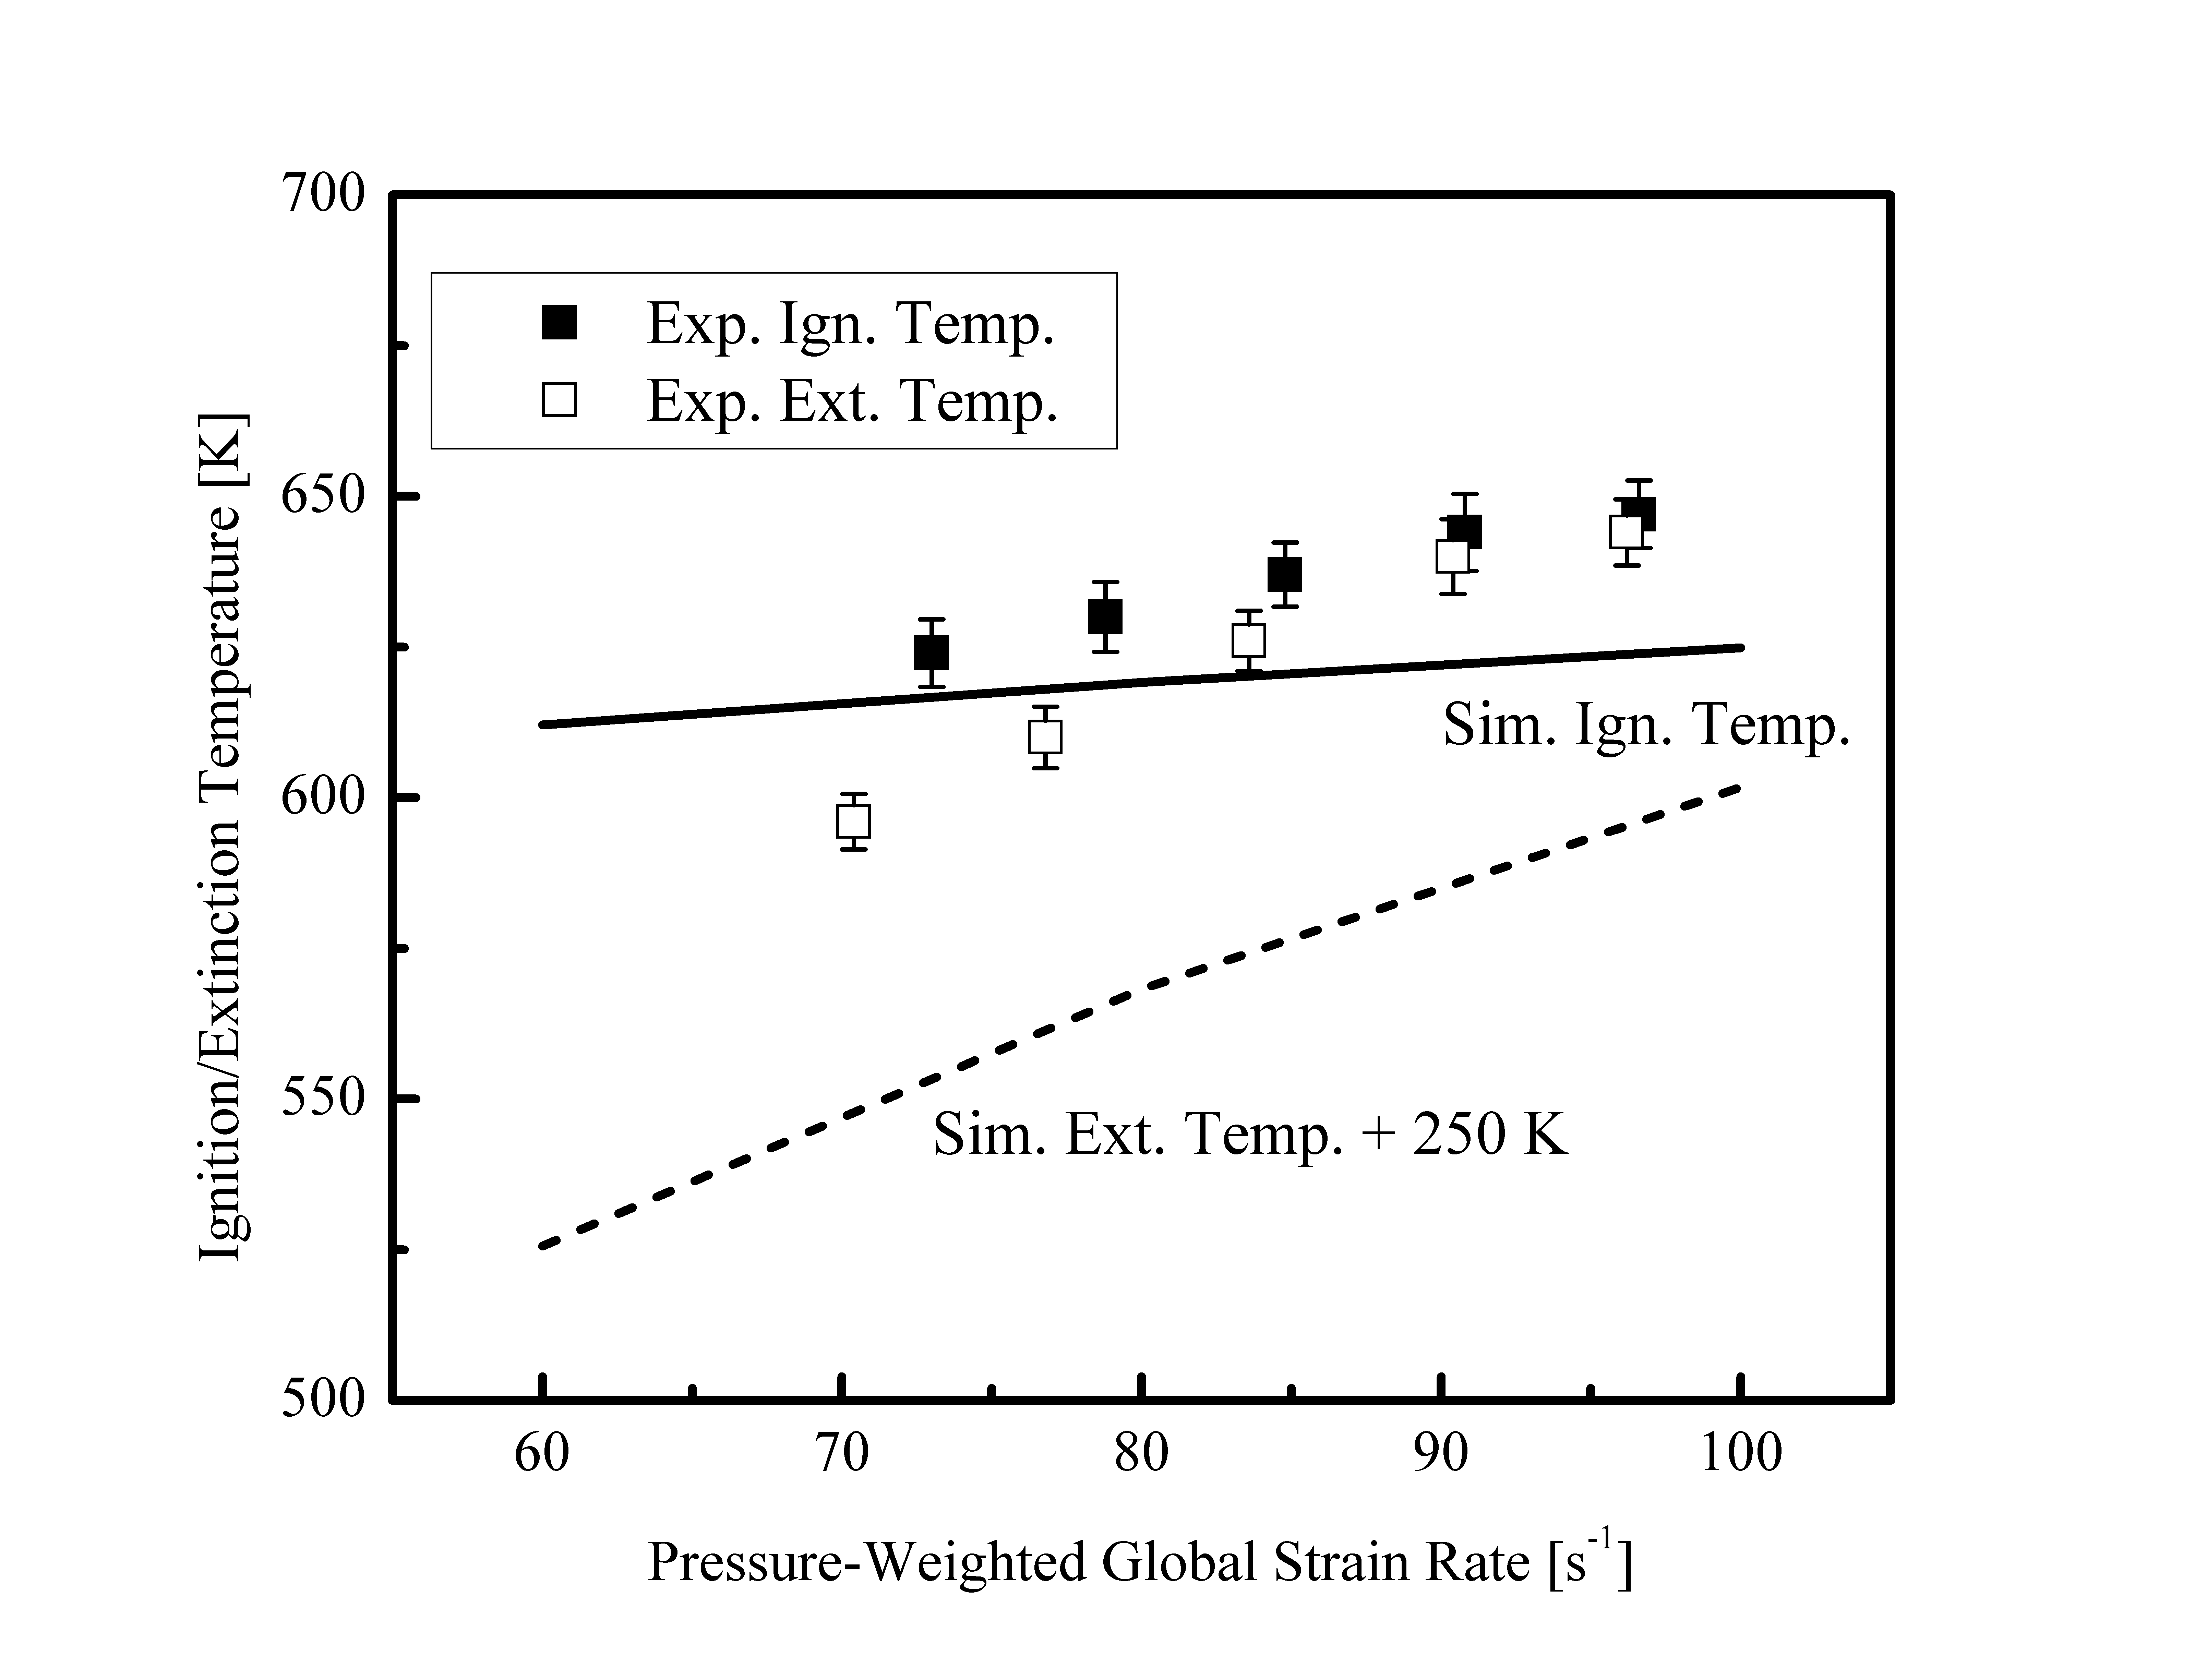
\includegraphics[width=1.0\textwidth]{ch-NTC/cmp_demo.png}
  \normalsize
  \caption{Experimental and computed ignition and extinction temperatures at 2 atm and various strain rates.  The computed extinction temperature is shifted up by 250 K for better illustration.  DME volume fraction in the fuel stream is 50\%, and the oxidizer stream is air.}
  \label{fig:cmp_demo}
\end{figure}

It is also apparent from Fig.~\ref{fig:cmp_demo} that while the experimental and computational results separately exhibit the anticipated physics, namely the extinction temperature is lower than the ignition temperature, and they both increase with increasing strain rate, the quantitative comparison between them is overall poor, both in magnitude as well as the strain-rate sensitivity. Detailed analysis of these discrepancies is deferred to Sec.~\ref{sec:NTC-uncertainty}. 


\subsection{Analysis of Thermal and Chemical Structures}\label{sec:NTC-structure}

In order to elucidate the dominant chemical pathways and evolution of the ignition and extinction processes, the three characteristic points on the S-curve of Fig.~\ref{fig:Scurve-hys}, which respectively represent the states prior to ignition (point I), steady burning (point S), and prior to extinction (point E), were chosen for structural analysis.

As shown in Fig.~\ref{fig:NTC-HRR}, the heat release just prior to the initiation of the cool flame is negligible, and the maximum temperature in the flow field is set by the oxidizer boundary.  For both steady flames at points S and E, there are reaction kernels delineated by the heat release profiles.  Based on the full width at half maximum of the heat release profile, a typical cool flame thickness is about 0.5 mm for the present conditions.  At point E, the heat release rate of the cool flame is higher than that at point S, for low-temperature chemistry is favored at relatively lower temperatures.  However, the steep gradient of the heat release profile indicates that heat loss to the boundary at point E is more pronounced compared to point S.  As the boundary temperature further decreases, such heat loss increases, and chemical reactions cannot keep up with heat loss from the reaction zone, leading to extinction due to the limited residence time in the strained flow.

\begin{figure}[t]
  \centering
  \scriptsize
  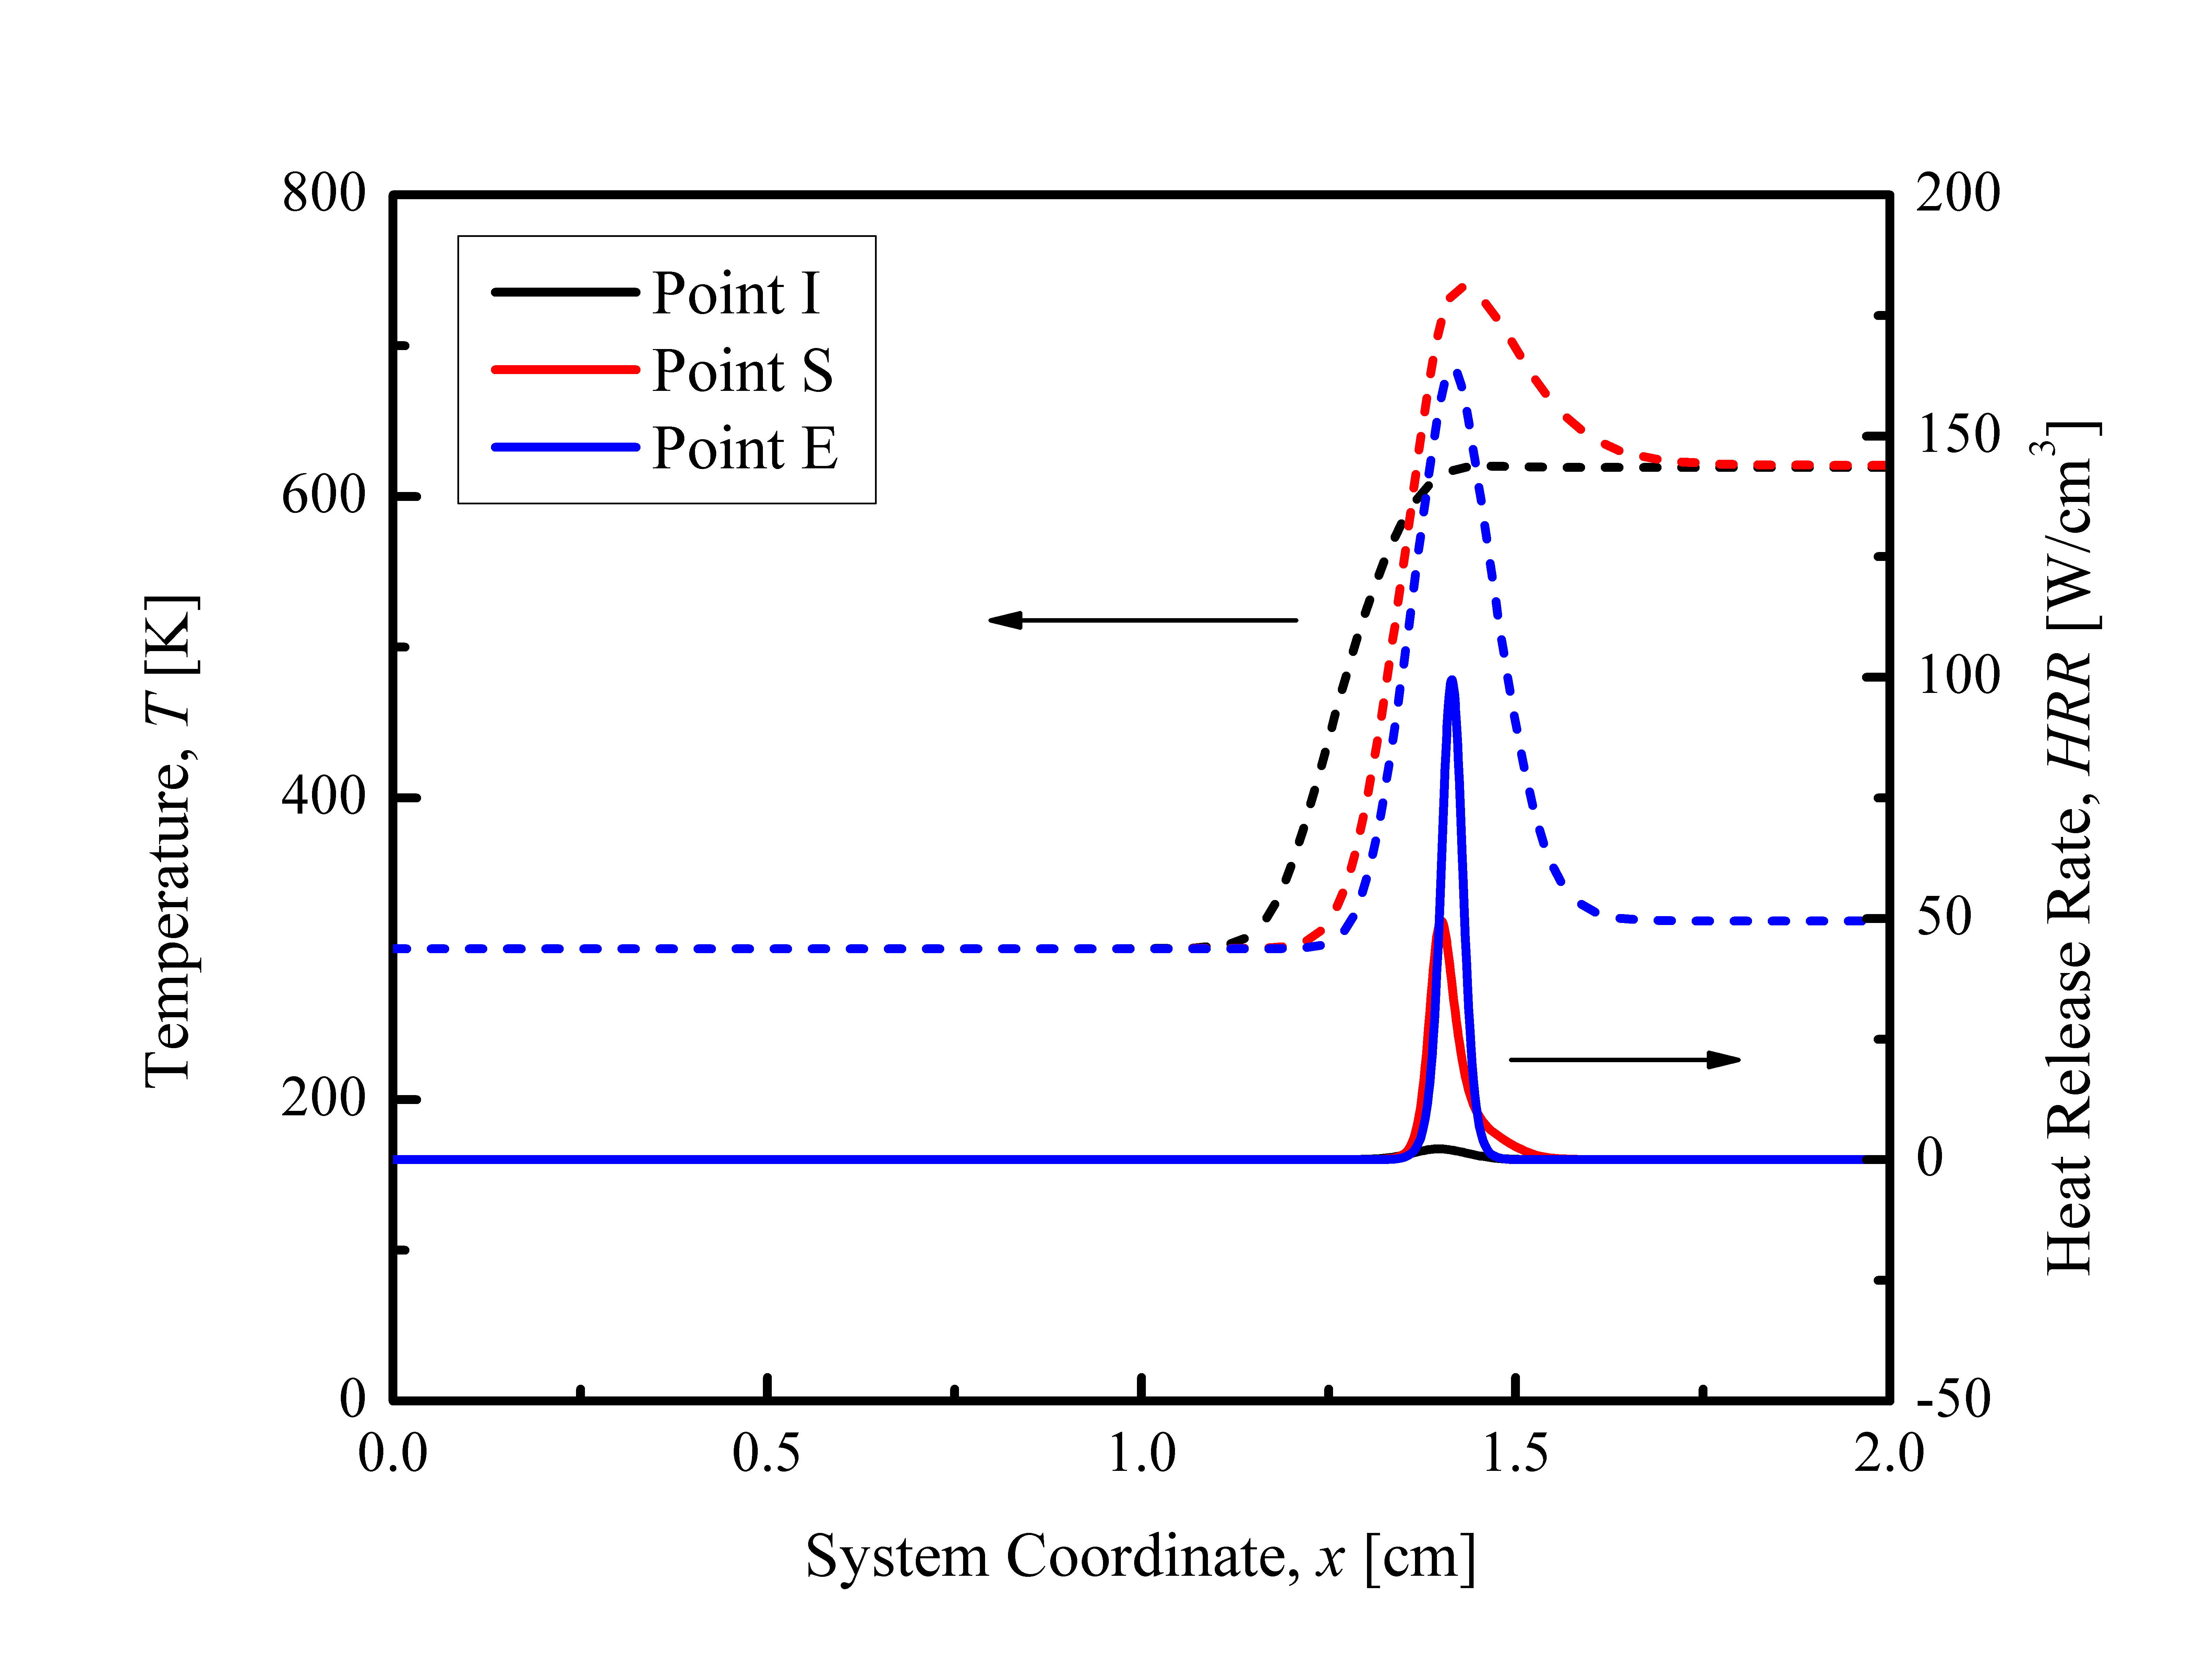
\includegraphics[width=1.0\textwidth]{ch-NTC/HRR.png}
  \normalsize
  \caption{Thermal structures in the computed flow field at three representative points on the S-curve shown in Fig.~\ref{fig:Scurve-hys}.  Fuel stream boundary conditions are specified at $x=0$ in the computation.}
  \label{fig:NTC-HRR}
\end{figure}

The profiles of three representative species, specifically, methoxymethylperoxy (CH$_3$OCH$_2$O$_2$), formaldehyde (CH$_2$O or HCHO), and hydroxyl (OH), were then investigated to elucidate the chemical structures at these three points, I, S, and E, as shown in Figs.~\ref{fig:NTC-species_a} to~\ref{fig:NTC-species_c}.  The methoxymethylperoxy radical was chosen because it is a representative species for the low-temperature chemistry~\cite{krisman15}.  Comparing the species profiles of the three states, it is seen that the CH$_3$OCH$_2$O$_2$ mass fraction increases upon flame initiation, and, similar to the heat release rate profile, its peak increases as extinction is approached.  Moreover, the profile broadens, for low-temperature chemistry is favored at reduced oxidizer boundary temperature.  Formaldehyde was selected because it is a major “product” of the cool flame, with its intensity manifested through its chemiluminescence~\cite{zhao16}.  It is then seen that: negligible CH$_2$O is formed prior to ignition, significant amount is formed in the steady flame, and the concentration and hence the intensity of chemiluminescence is reduced as extinction is approached. Finally, the hydroxyl radical was chosen because it represents high-temperature flame chemistry and is also an important radical formed during the chain branching reactions of the low-temperature chemistry.  It is then noted that the peak mass fraction of OH is several orders of magnitude smaller than those in a typical hot flame.  The ignition of a cool flame is initiated with a peak formation of OH, which subsequently decreases upon ignition.  With subsequent heat release from the cool flame, a second peak of OH mass fraction emerges on the oxidizer side of the cool flame peak, which is responsible for the initiation of the hot flame at higher boundary temperatures~\cite{law12}.

\begin{figure}[t]
  \centering
  \scriptsize
  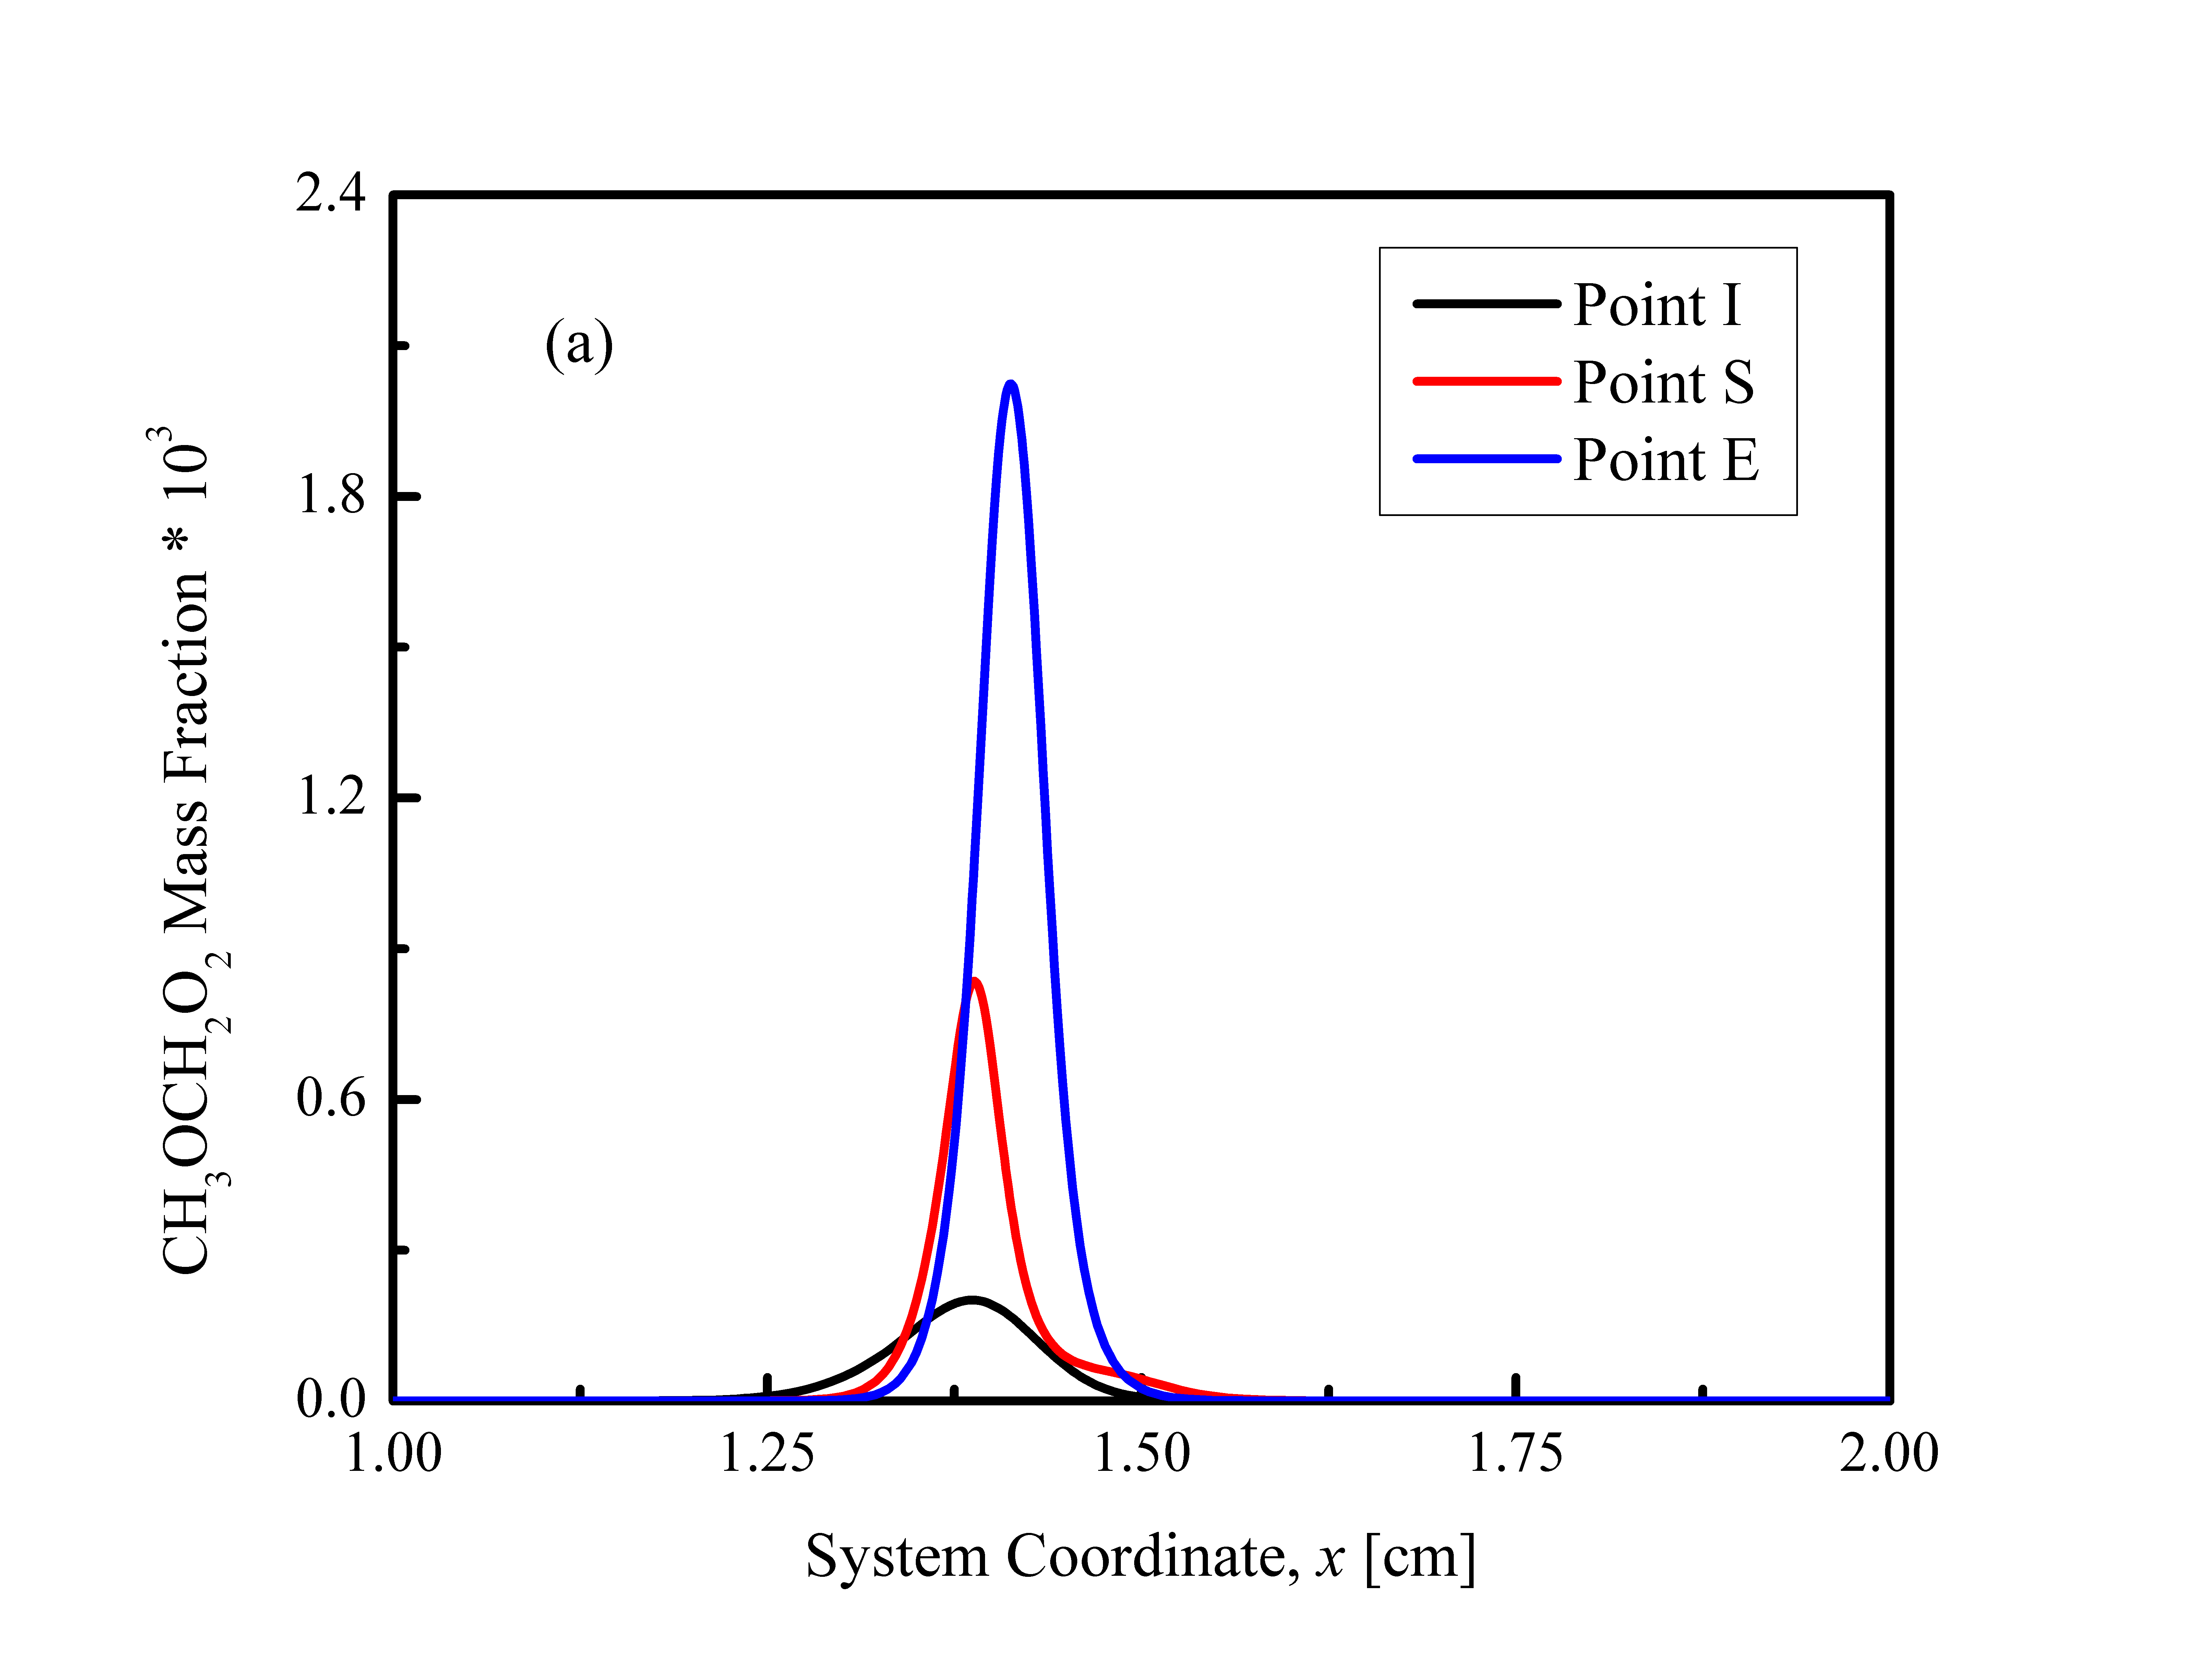
\includegraphics[width=1.0\textwidth]{ch-NTC/sp_a.png}
  \normalsize
  \caption{Species profiles in the computed flow field at three representative points on the S-curve shown in Fig.~\ref{fig:Scurve-hys}: methoxymethylperoxy radical.  Fuel stream boundary conditions are specified at $x=0$ in the computation.}
  \label{fig:NTC-species_a}
\end{figure}

\begin{figure}[t]
  \centering
  \scriptsize
  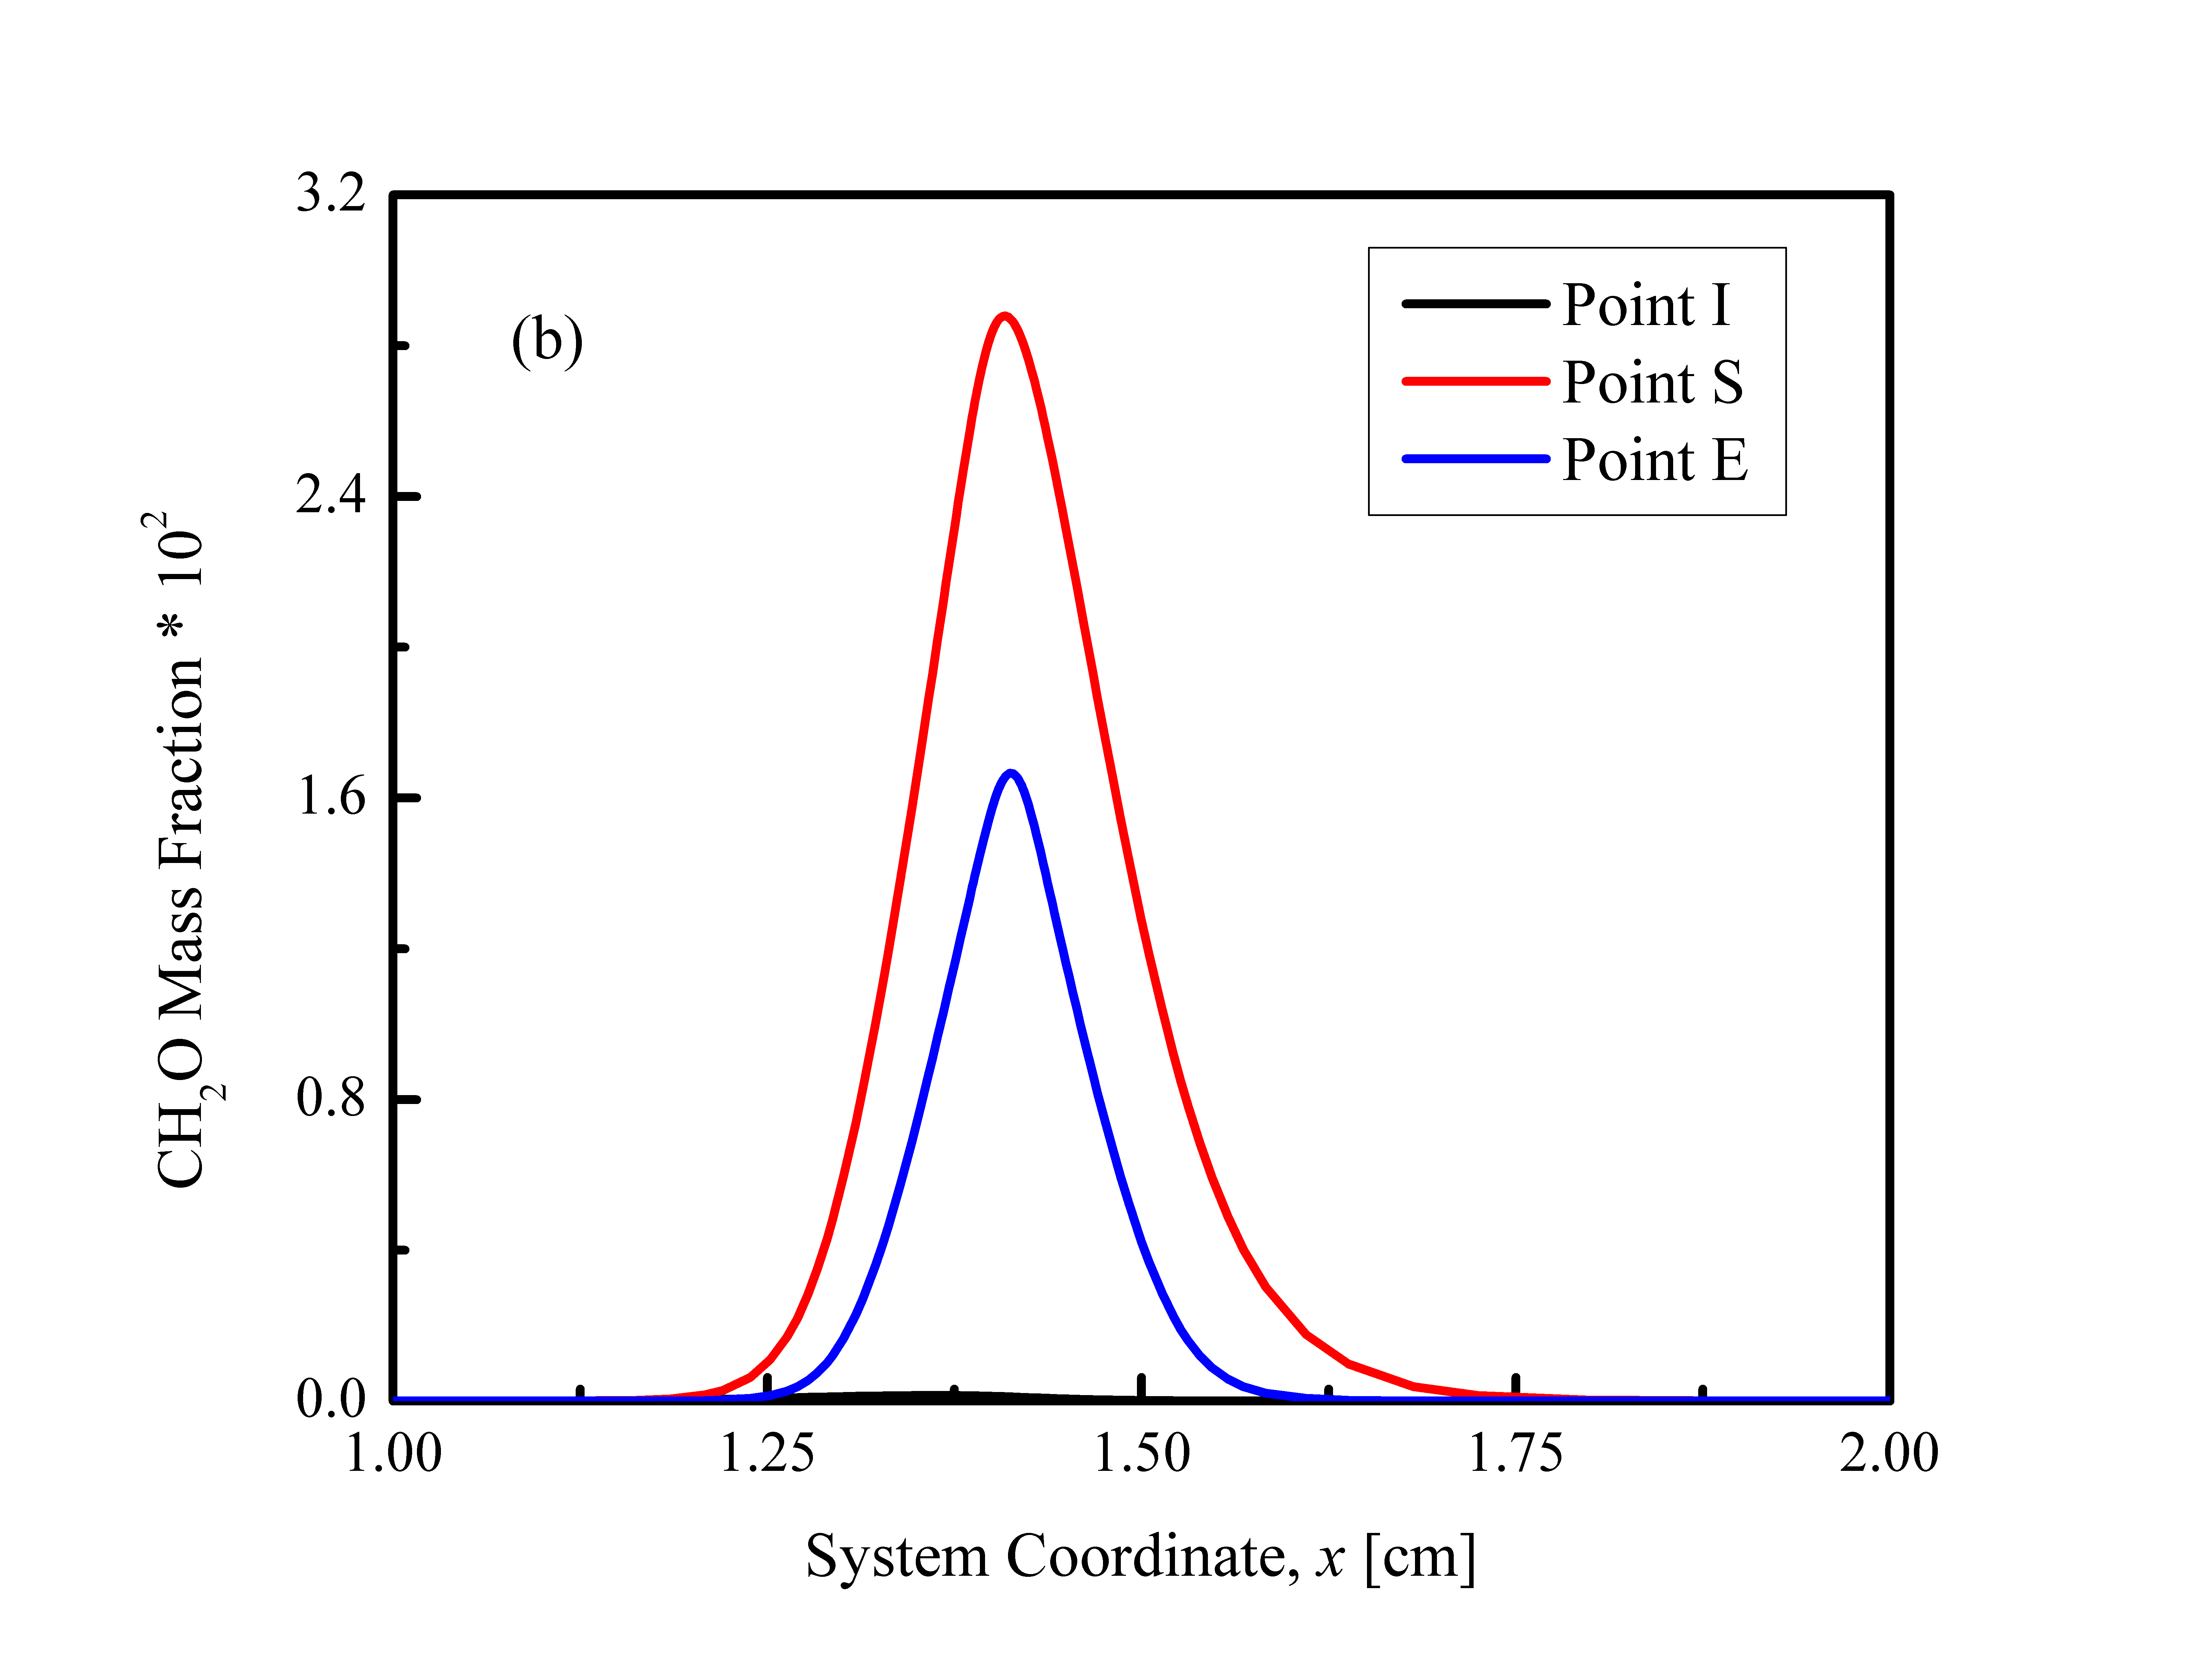
\includegraphics[width=1.0\textwidth]{ch-NTC/sp_b.png}
  \normalsize
  \caption{Species profiles in the computed flow field at three representative points on the S-curve shown in Fig.~\ref{fig:Scurve-hys}: formaldehyde.  Fuel stream boundary conditions are specified at $x=0$ in the computation.}
  \label{fig:NTC-species_b}
\end{figure}

\begin{figure}[t]
  \centering
  \scriptsize
  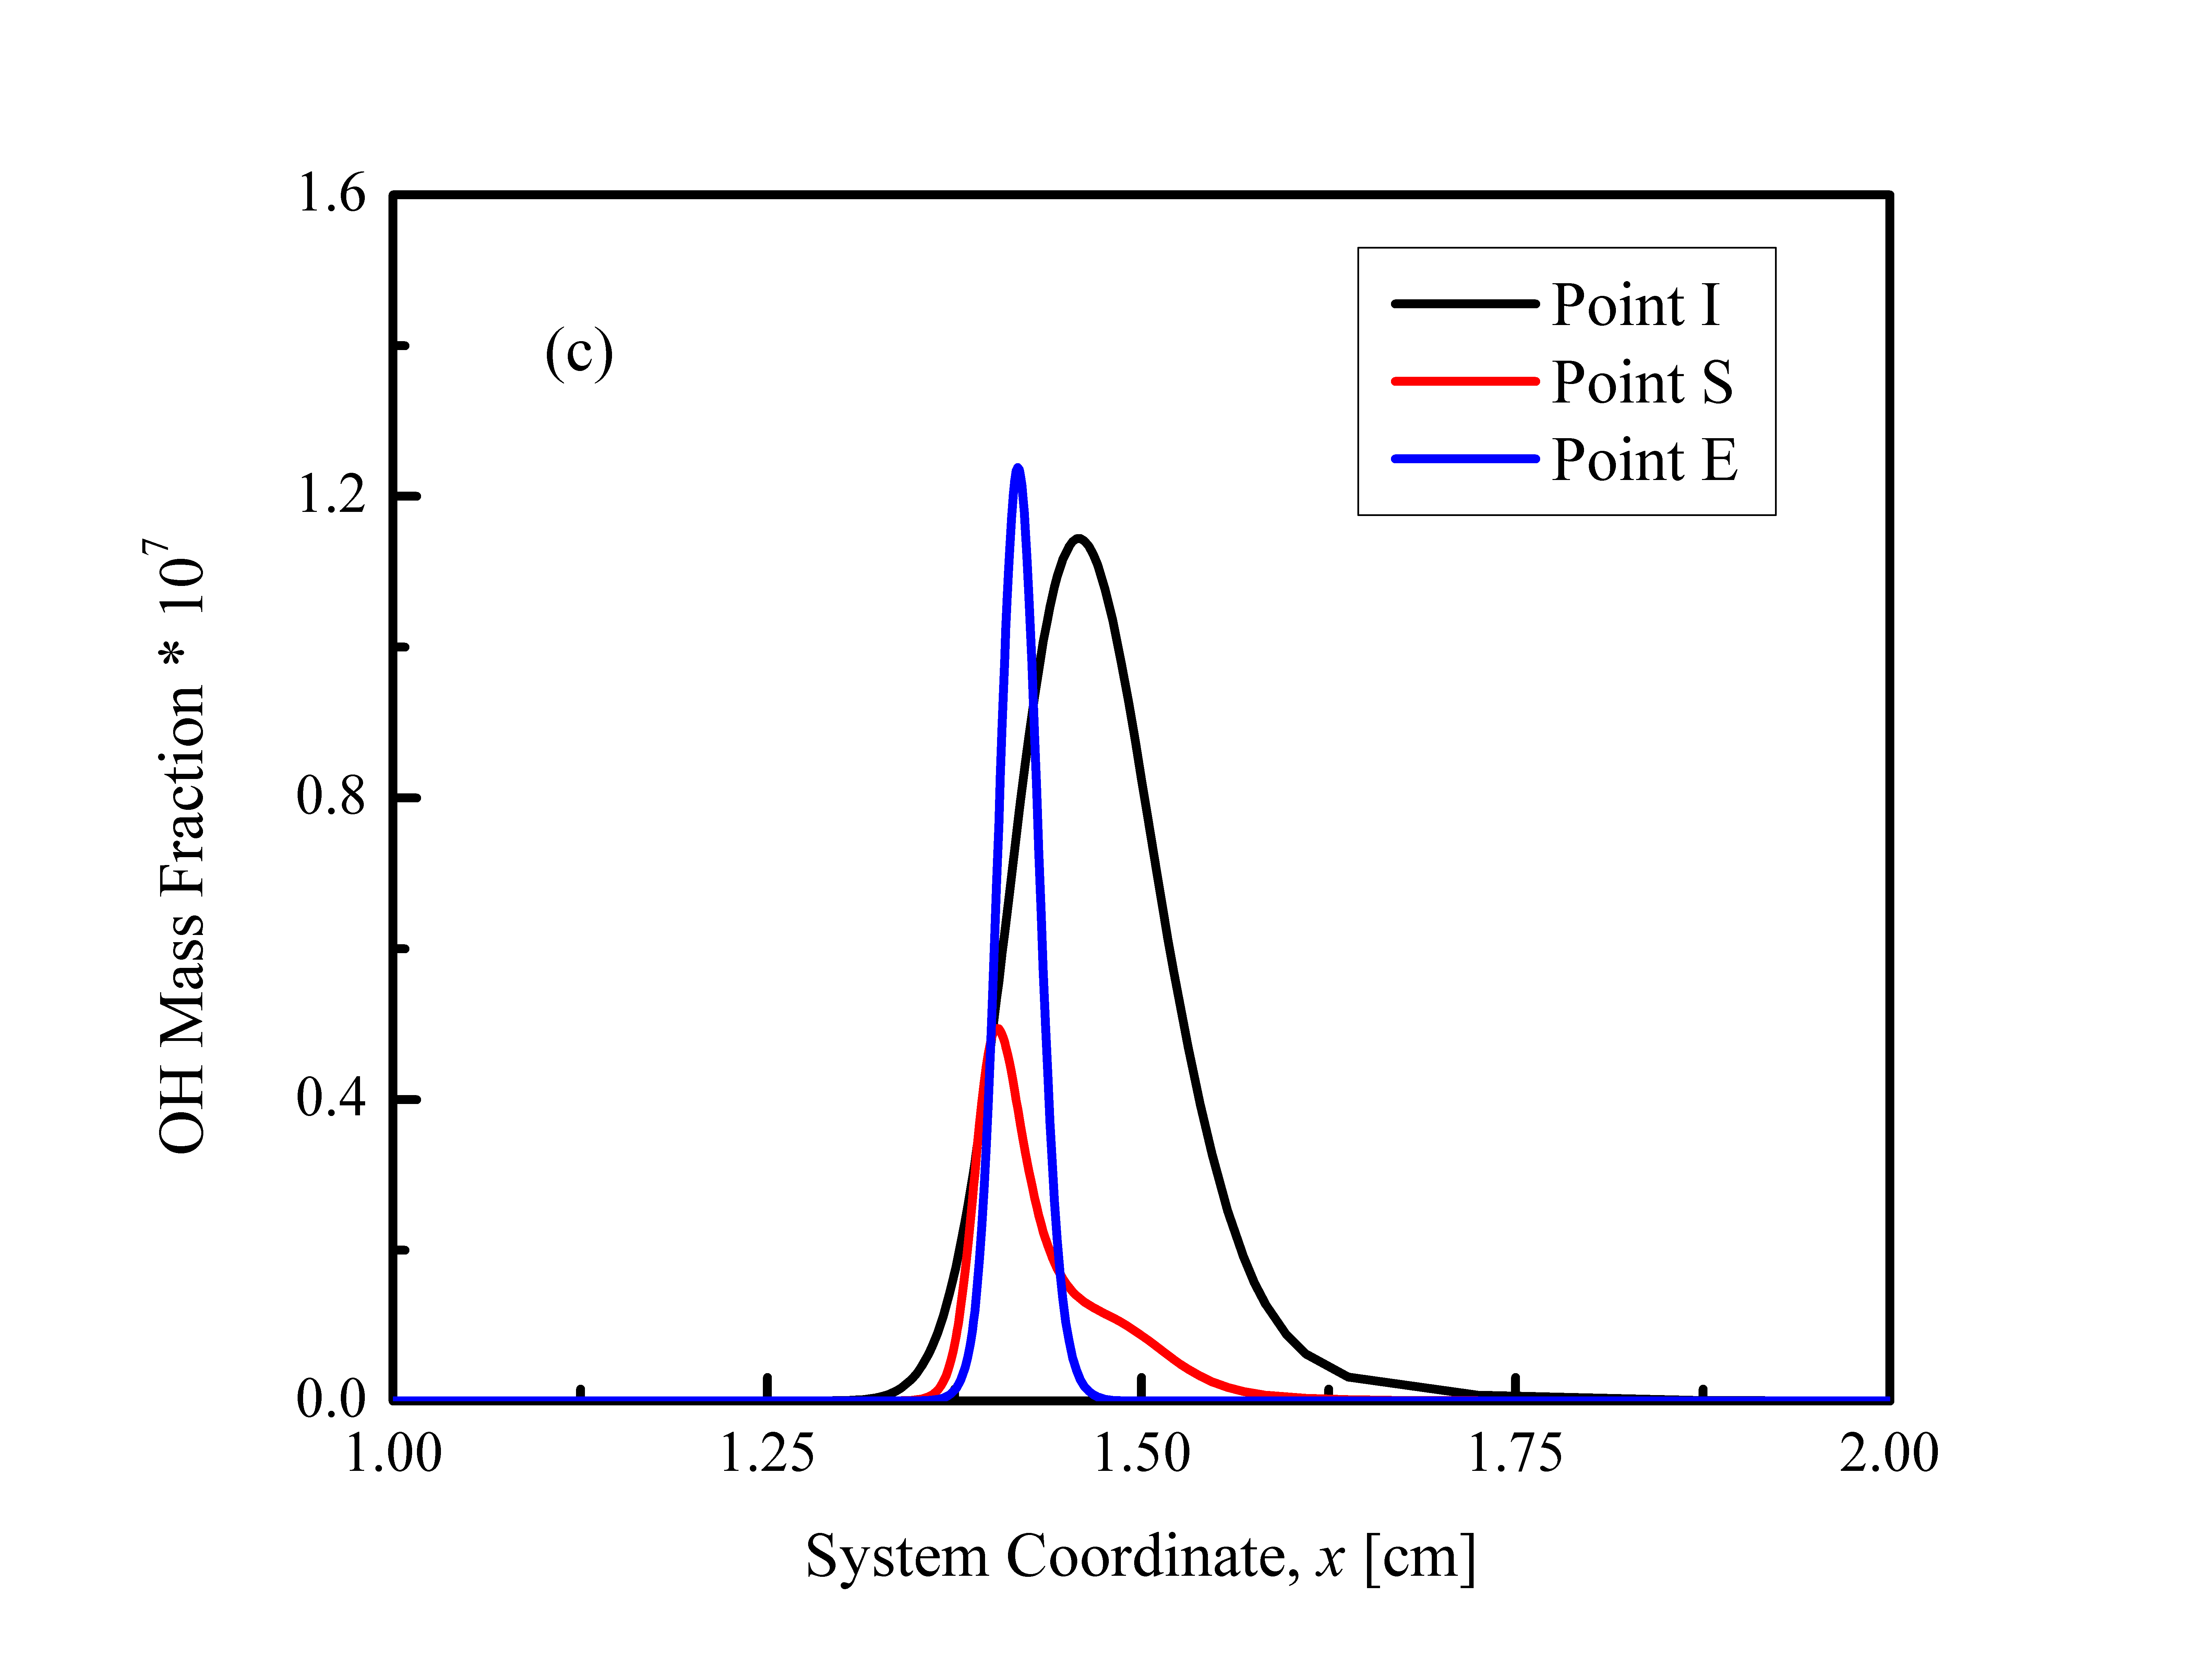
\includegraphics[width=1.0\textwidth]{ch-NTC/sp_c.png}
  \normalsize
  \caption{Species profiles in the computed flow field at three representative points on the S-curve shown in Fig.~\ref{fig:Scurve-hys}: hydroxyl radical.  Fuel stream boundary conditions are specified at $x=0$ in the computation.}
  \label{fig:NTC-species_c}
\end{figure}

Finally, sensitivity analysis was conducted to elucidate the evolution of the dominant chemical pathways during the ignition and extinction processes.  The maximum temperature was chosen as the target for sensitivity analysis, and the ratio of the relative change of the maximum temperature to that of the Arrhenius factor of each reaction being perturbed was defined as the sensitivity coefficient.  The sensitivity coefficients of all the reactions considered in the chemical mechanism were normalized by the maximum value such that the normalized sensitivity coefficient is bounded by -1 and 1 to allow for comparisons between the cases.

The normalized sensitivity coefficients ranked by their absolute values for states I, S, and E in Fig.~\ref{fig:Scurve-hys} are shown in Fig.~\ref{fig:NTC-SA}.  At all three states, low-temperature chemistry is dominant, with the absence of the typical high-temperature chain branching reactions such as $\rm{H} + \rm{O}_2 \Longleftrightarrow \rm{OH} + \rm{O}$.  Similar to the ignition analysis in Sec.~\ref{sec:NTC-4.2}, the isomerization reaction $\rm{CH}_3\rm{OCH}_2\rm{O}_2 \Longleftrightarrow \rm{CH}_2\rm{OCH}_2\rm{O}_2\rm{H}$ and the oxygen addition reaction $\rm{CH}_2\rm{OCH}_2\rm{O}_2\rm{H} + \rm{O}_2 \Longleftrightarrow \rm{O}_2\rm{CH}_2\rm{OCH}_2\rm{O}_2\rm{H}$ promote ignition, while the reaction $\rm{CH}_2\rm{OCH}_2\rm{O}_2\rm{H} \Longleftrightarrow \rm{OH} + 2\rm{CH}_2\rm{O}$ retards it.  However, for the steady cool flames corresponding to points S and E, the relative importance of these reactions shifts.  First, $\rm{CH}_2\rm{OCH}_2\rm{O}_2\rm{H} + \rm{O}_2 \Longleftrightarrow \rm{O}_2\rm{CH}_2\rm{OCH}_2\rm{O}_2\rm{H}$ becomes even more important in steady cool flames.  Since the maximum temperature was chosen as the target to evaluate the sensitivity, the exothermic reaction $\rm{CH}_2\rm{OCH}_2\rm{O}_2\rm{H} + \rm{O}_2 \Longleftrightarrow \rm{O}_2\rm{CH}_2\rm{OCH}_2\rm{O}_2\rm{H}$ demonstrates a large positive sensitivity coefficient.  Conversely, at ignition, reactions that finally lead to radical runaway are more important, for heat release from the mixing layer is negligible at this state, as shown in Fig.~\ref{fig:NTC-HRR}.  Second, the isomerization reaction $\rm{CH}_3\rm{OCH}_2\rm{O}_2 \Longleftrightarrow \rm{CH}_2\rm{OCH}_2\rm{O}_2\rm{H}$ becomes important again near extinction, for, at extinction, the radical production rates barely keep up with the transport losses and the chain carrying limiting step becomes crucial again.

\begin{figure}[t]
  \centering
  \scriptsize
  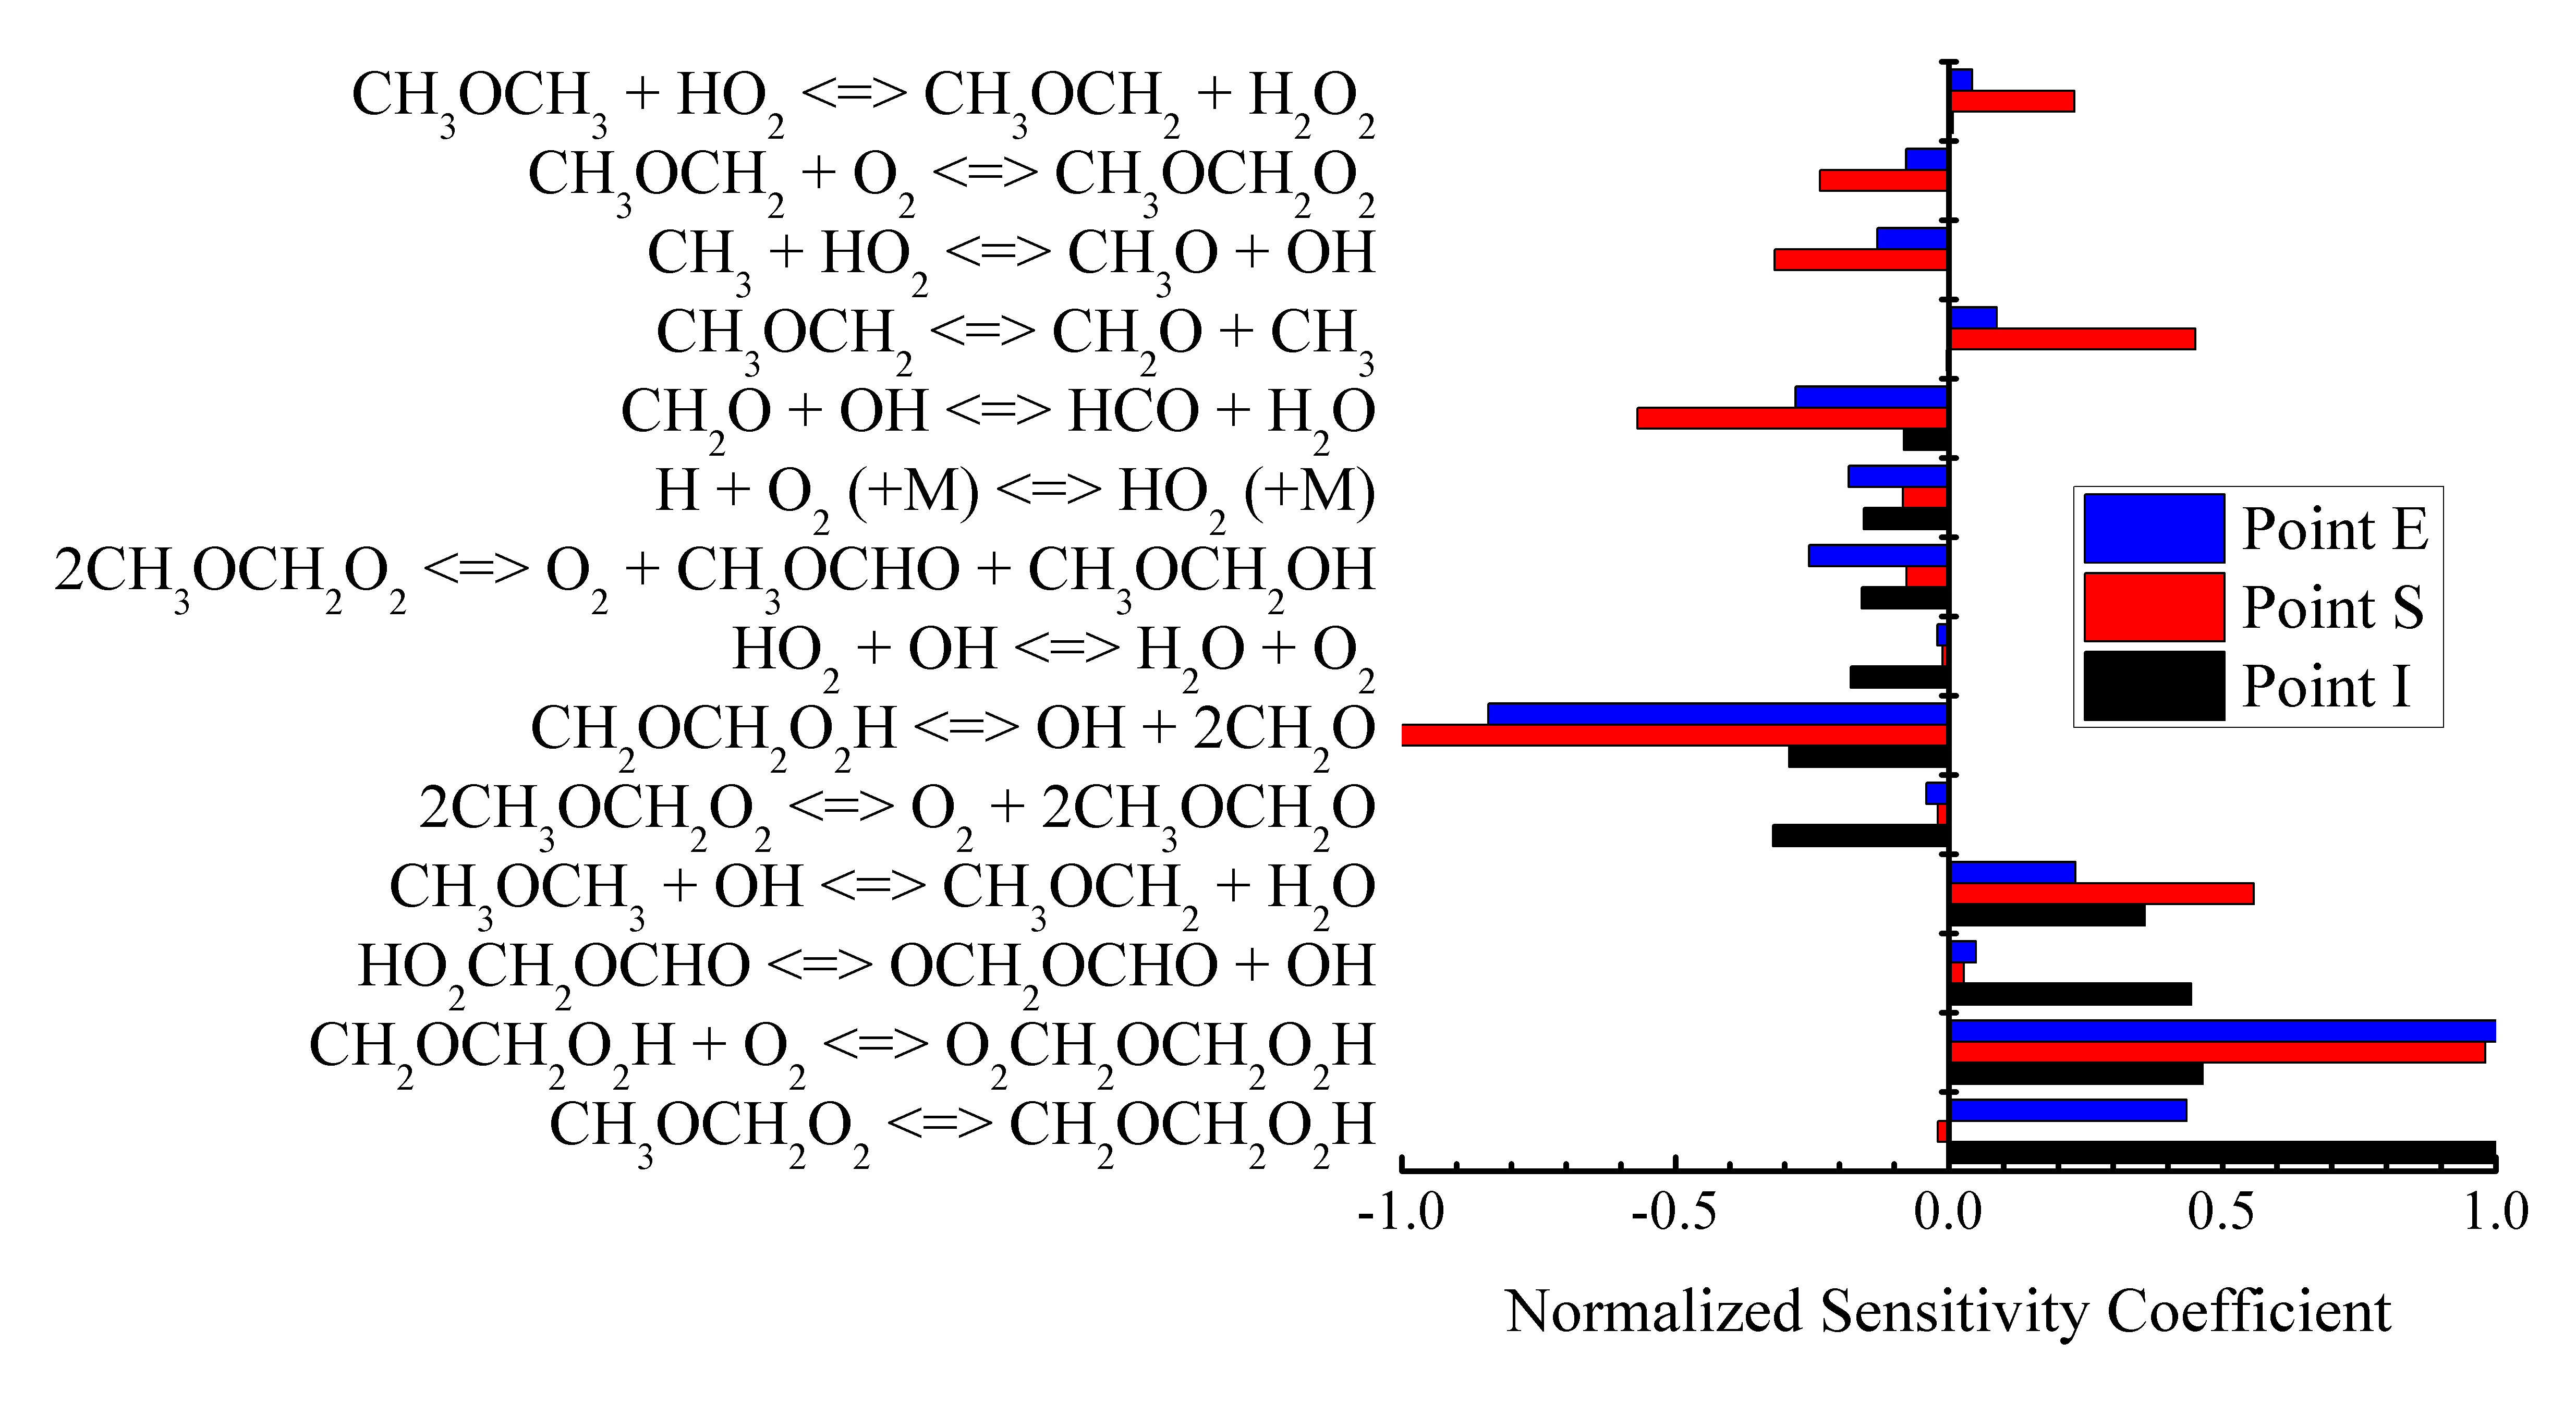
\includegraphics[width=1.0\textwidth]{ch-NTC/SA.png}
  \normalsize
  \caption{Reaction sensitivity analysis at three representative points on the S-curve shown in Fig.~\ref{fig:Scurve-hys}.}
  \label{fig:NTC-SA}
\end{figure}

\subsection{Uncertainty Analysis}\label{sec:NTC-uncertainty}

As noted in Fig.~\ref{fig:cmp_demo}, while the computation is able to capture the experimental observation of the hysteretic feature of ignition and extinction, as well as the increasing trend of ignition and extinction temperatures with increasing strain rate, the quantitative agreement is rather poor.  Specifically, the ignition temperature is slightly overpredicted; its sensitivity to strain rate, indicated by the slope of the ignition temperature profile, is substantially underpredicted; and, most importantly, the extinction temperature is significantly underpredicted. Upon extensive exploration of the various experimental and modeling factors that could contribute to such substantial disagreements, the uncertainty of the low-temperature chemistry used in the computation has surfaced to be the dominant factor.

To demonstrate the effects of such uncertainty and since the ignition temperatures of the cool flames are fairly well captured, it is reasonable to inspect reactions with large sensitivity coefficients in Fig.~\ref{fig:NTC-SA} for the cool flames.  This leads to the identification of the reactions: $\rm{CH}_2\rm{OCH}_2\rm{O}_2\rm{H} + \rm{O}_2 \Longleftrightarrow \rm{O}_2\rm{CH}_2\rm{OCH}_2\rm{O}_2\rm{H}$ and $\rm{CH}_2\rm{OCH}_2\rm{O}_2\rm{H} \Longleftrightarrow \rm{OH} + 2\rm{CH}_2\rm{O}$.  Since cool flames appear to be more robust to extinguish, the preexponential factors of these two reactions were modified by respectively reducing and increasing to 70\% and 200\% of their original values.

\begin{figure}[t]
  \centering
  \scriptsize
  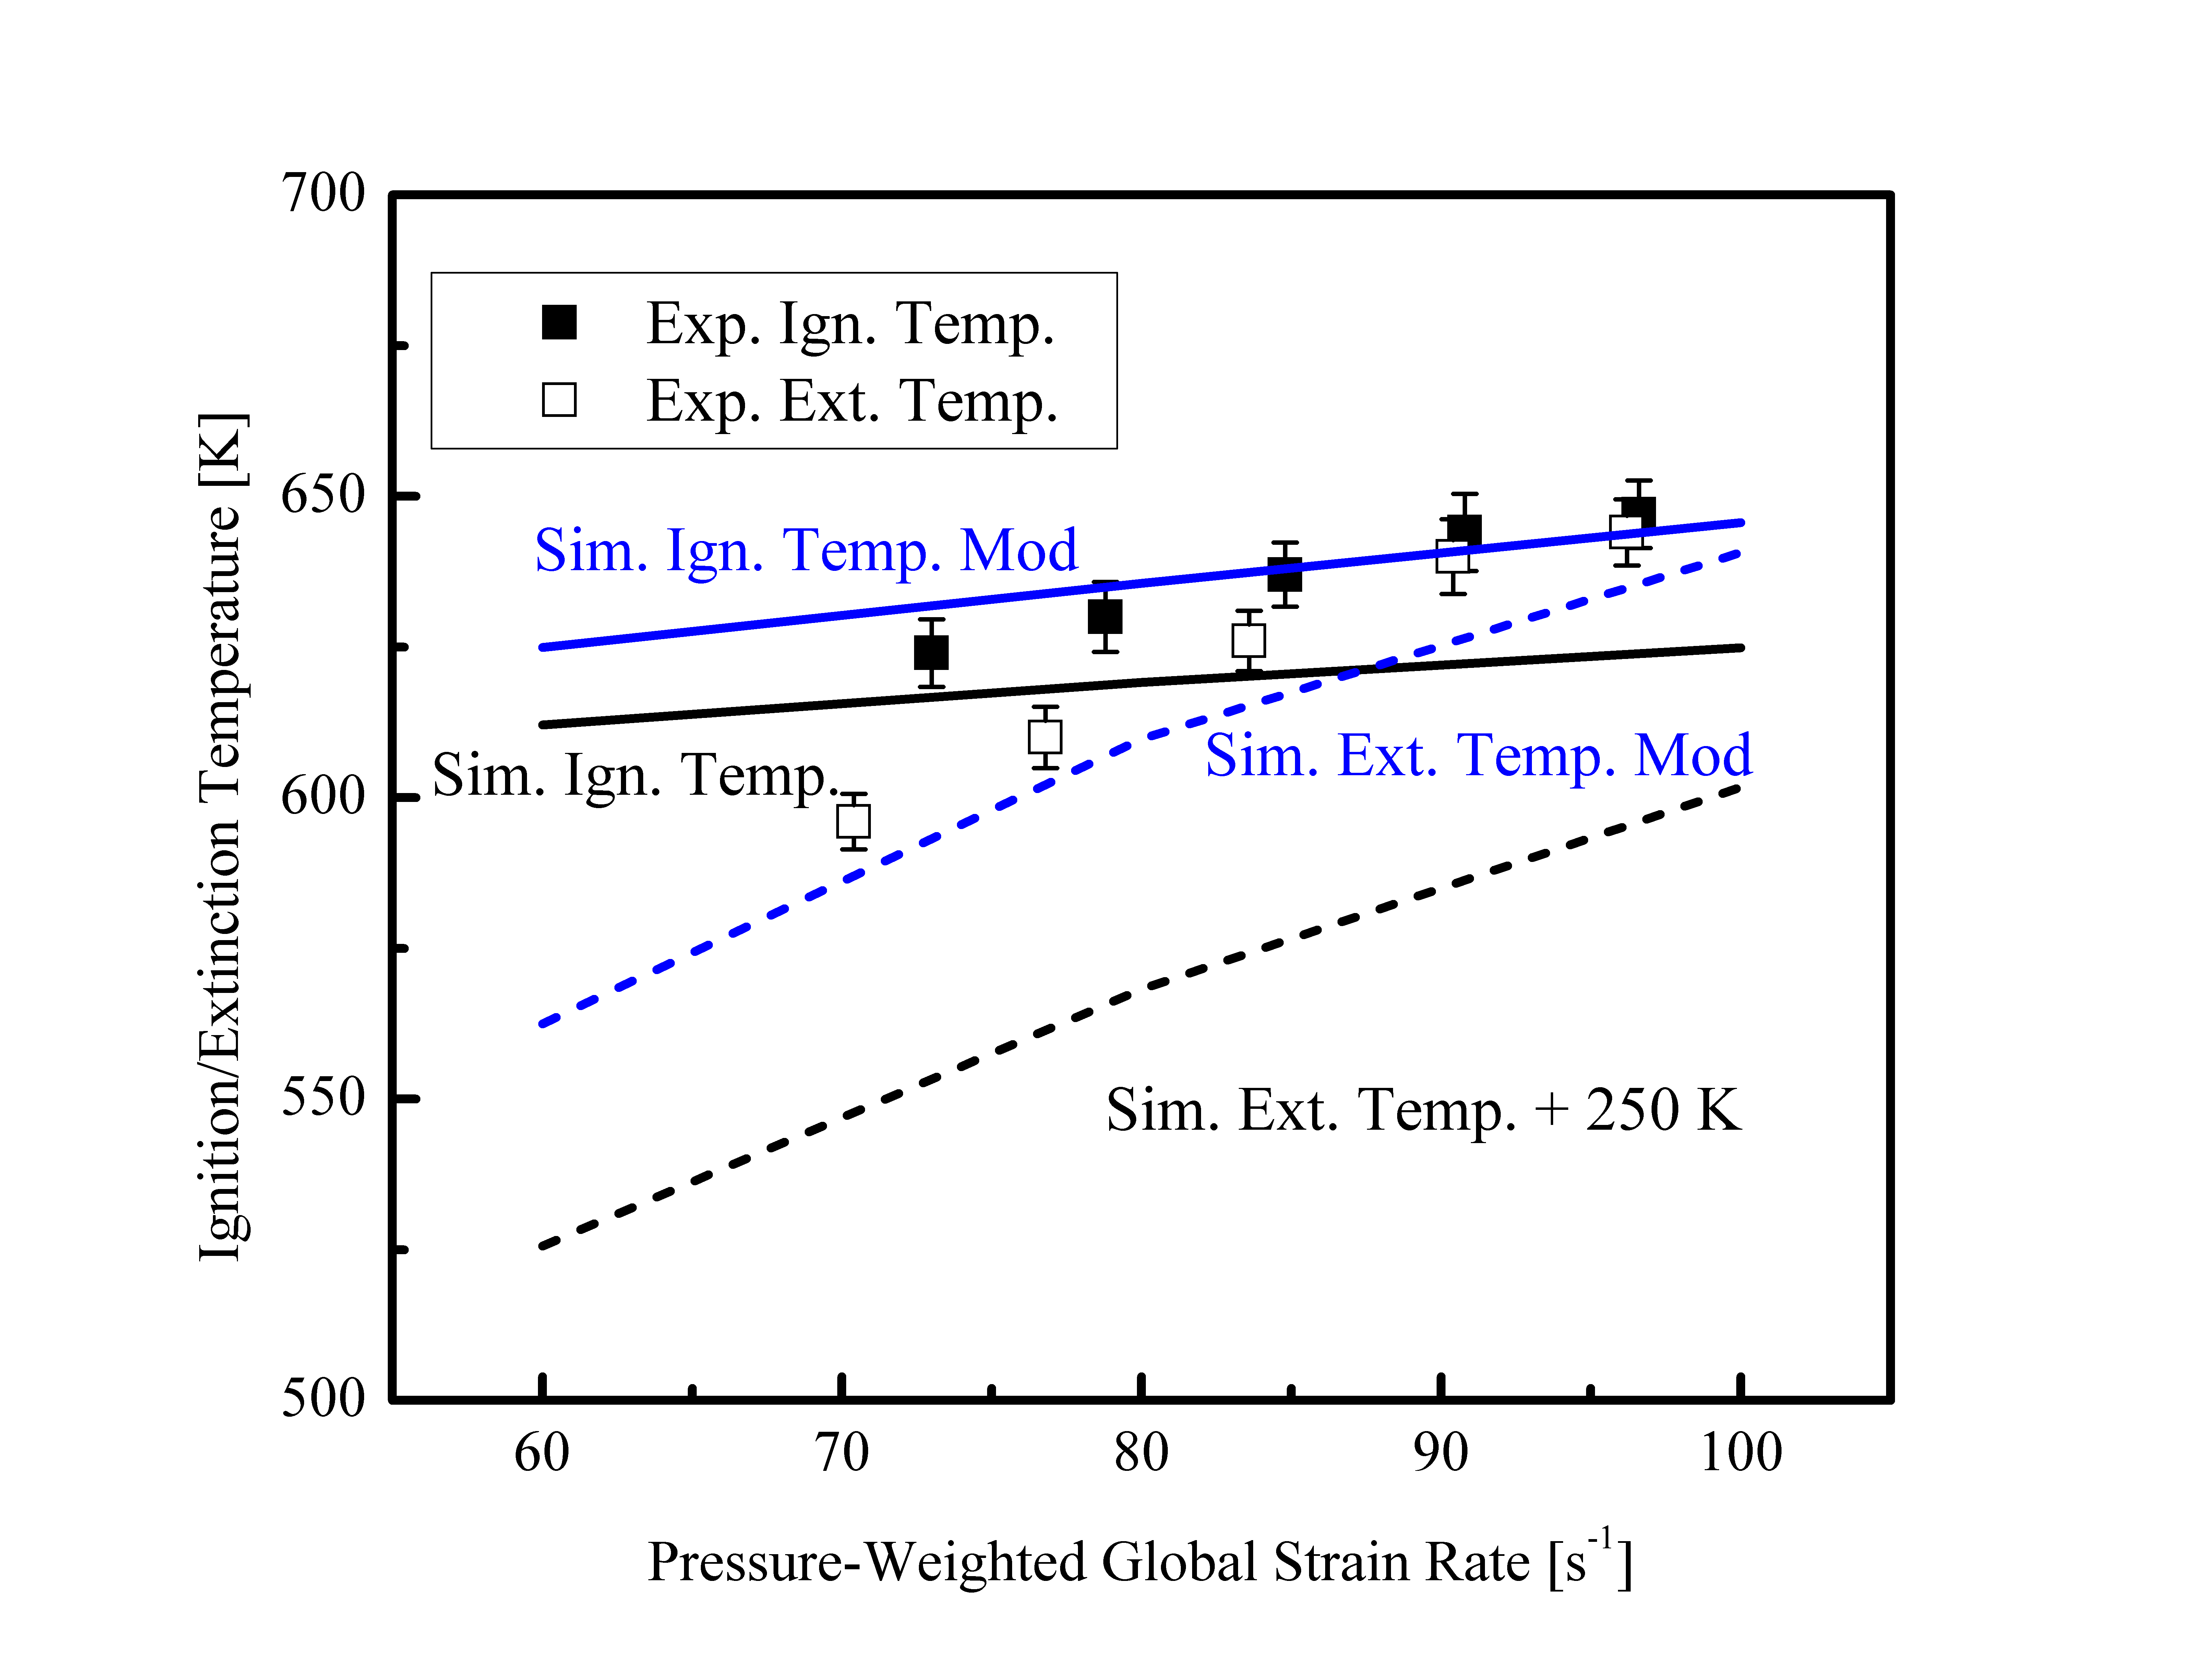
\includegraphics[width=1.0\textwidth]{ch-NTC/cmp_demo_mod.png}
  \normalsize
  \caption{Revisit of Fig.~\ref{fig:cmp_demo} with modified reaction rates in the chemical mechanism.  Note that the line plots with the modified reaction rates are presented without shifting.}
  \label{fig:cmp_demo_mod}
\end{figure}

Figure~\ref{fig:cmp_demo_mod} then shows that both qualitative and quantitative agreements between experiments and computations are achieved with the modified reaction parameters.  Specifically, although the magnitude of the ignition temperature is not very sensitive to the modifications, as expected, its sensitivity to increasing strain rate is enhanced, for the modifications essentially slow down the low-temperature chemistry such that the sensitivity to finite residence time is more pronounced.  More importantly, it is seen that good agreement is also achieved for the highly sensitive extinction temperatures, significantly boosting their values but without changing the sensitivity to the strain rate variation.

While the above results appear to be encouraging, it should be noted that the objective of this study is not to propose an improved chemical model with the modified kinetic parameters.  What has however been demonstrated is the sensitive nature of the low-temperature chemistry, in that substantial change in the global response can result with even small changes in these preexponential factors. In this regard, it is further noted that, during the development of the low-temperature chemical model, the validation data is limited to those from homogeneous systems. Clearly additional validation data on cool flames covering a wider range of conditions, which are inherently present in flame systems, is needed for the eventual development of a viable chemical model.

Another factor that could potentially affect the accuracy of the comparison between the experimental and computational results is the experimental detection limit of the UV camera, which could be too high compared to the chemiluminescence emission of the cool flame near extinction.  Since the hysteresis temperature window was observed in the experiment at various conditions, the detection threshold of the UV camera should be lower than the chemiluminescence intensity of the steady cool flame upon ignition.  Consequently, the ignition temperatures for these cases should be well captured.  However, the lower bound of the hysteresis temperature window could be limited by the detection threshold, and therefore, the actual extinction temperatures might not be captured accurately.

\subsection{Effects of Pressure and Oxygen Concentration}

\begin{figure}[t]
  \centering
  \scriptsize
  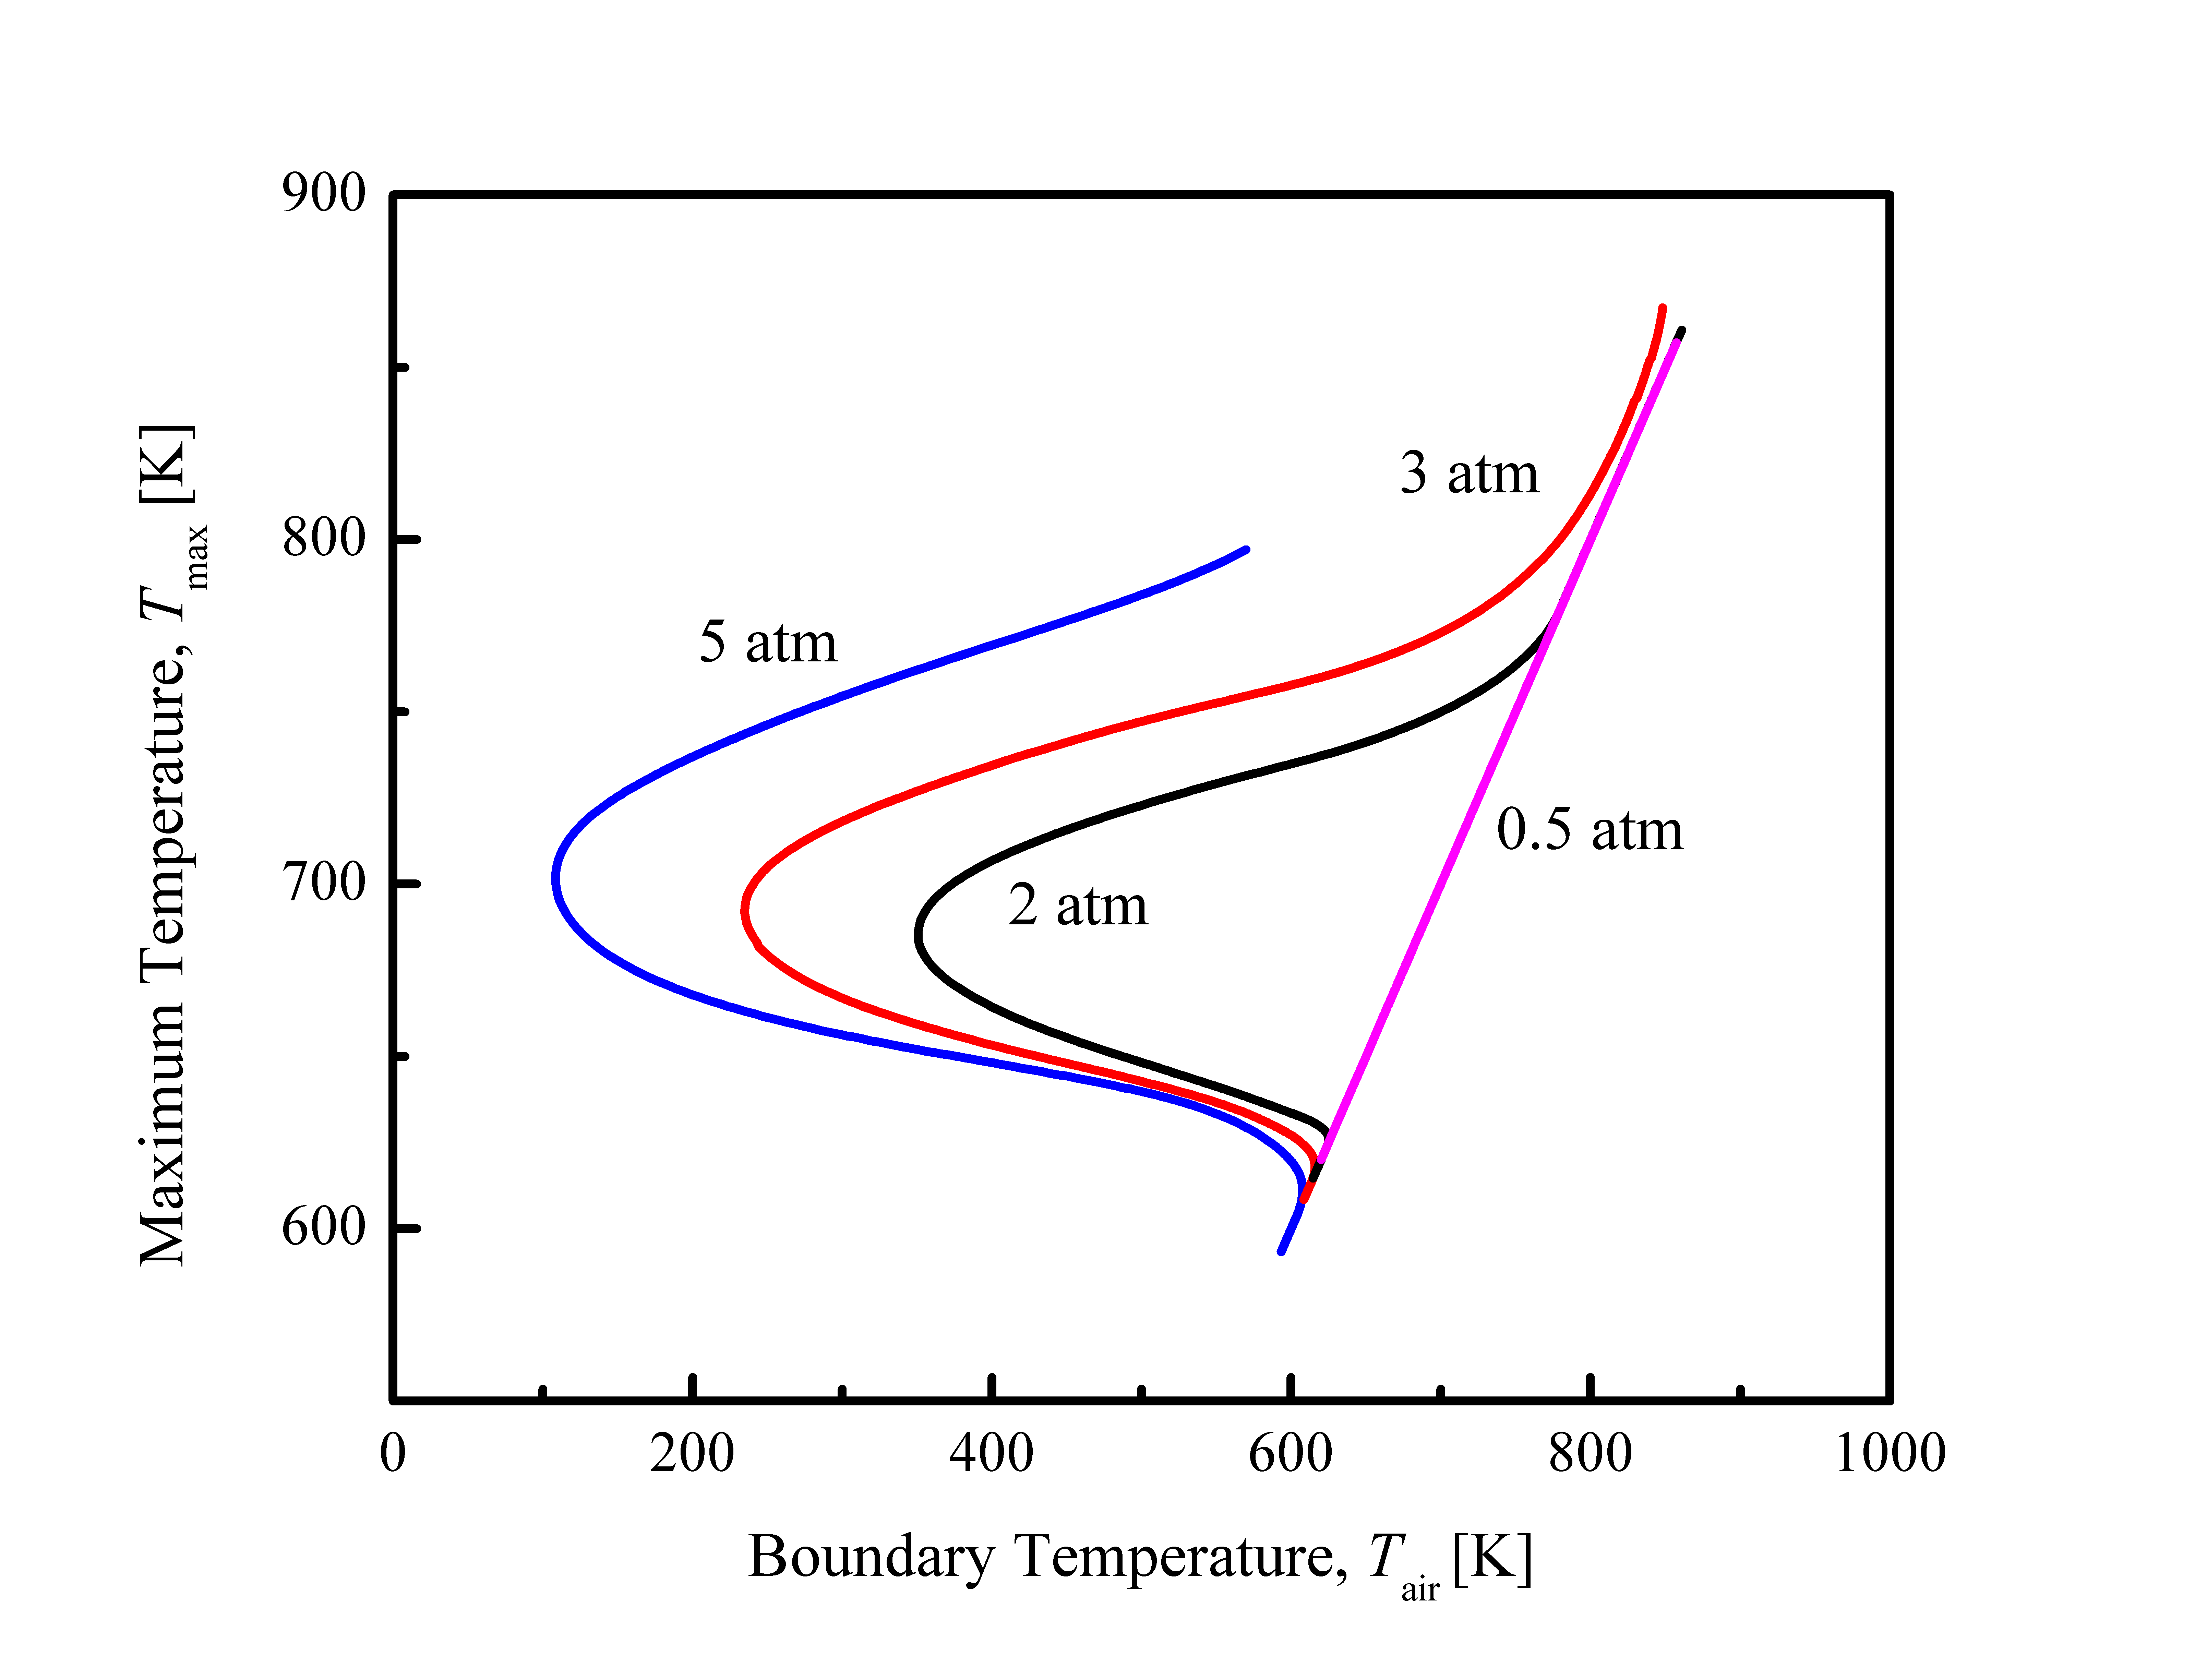
\includegraphics[width=1.0\textwidth]{ch-NTC/eff_P.png}
  \normalsize
  \caption{S-curve analysis for various ambient pressures and pressure-weighted strain rate of 100 /s.  DME volume fraction in the fuel stream is 50\%, and the oxidizer stream is air.}
  \label{fig:eff_P}
\end{figure}

The effects of ambient pressure and oxygen concentration in the oxidizer stream on the ignition and extinction of the cool flames were also investigated.  Pressure effects were first computationally studied by fixing the oxygen mole fraction in the oxidizer stream at 21\% and fixing the pressure-weighted strain rate at 100 /s, as shown in Fig.~\ref{fig:eff_P}.  It is seen that, as the pressure increases from 2 to 5 atm, the ignition temperature decreases and the heat release from the cool flame becomes more pronounced, as indicated by the temperature differences between the ignition turning point and the point on the cool flame branch with the same boundary temperature.  Moreover, the extinction turning point shifts to a lower boundary temperature, resulting in an extended hysteresis temperature window.  Conversely, the extent of the low-temperature chemistry governed S-curve hysteresis diminishes with decreasing pressure, leading to its absence at 0.5 atm.

\begin{figure}[t]
  \centering
  \scriptsize
  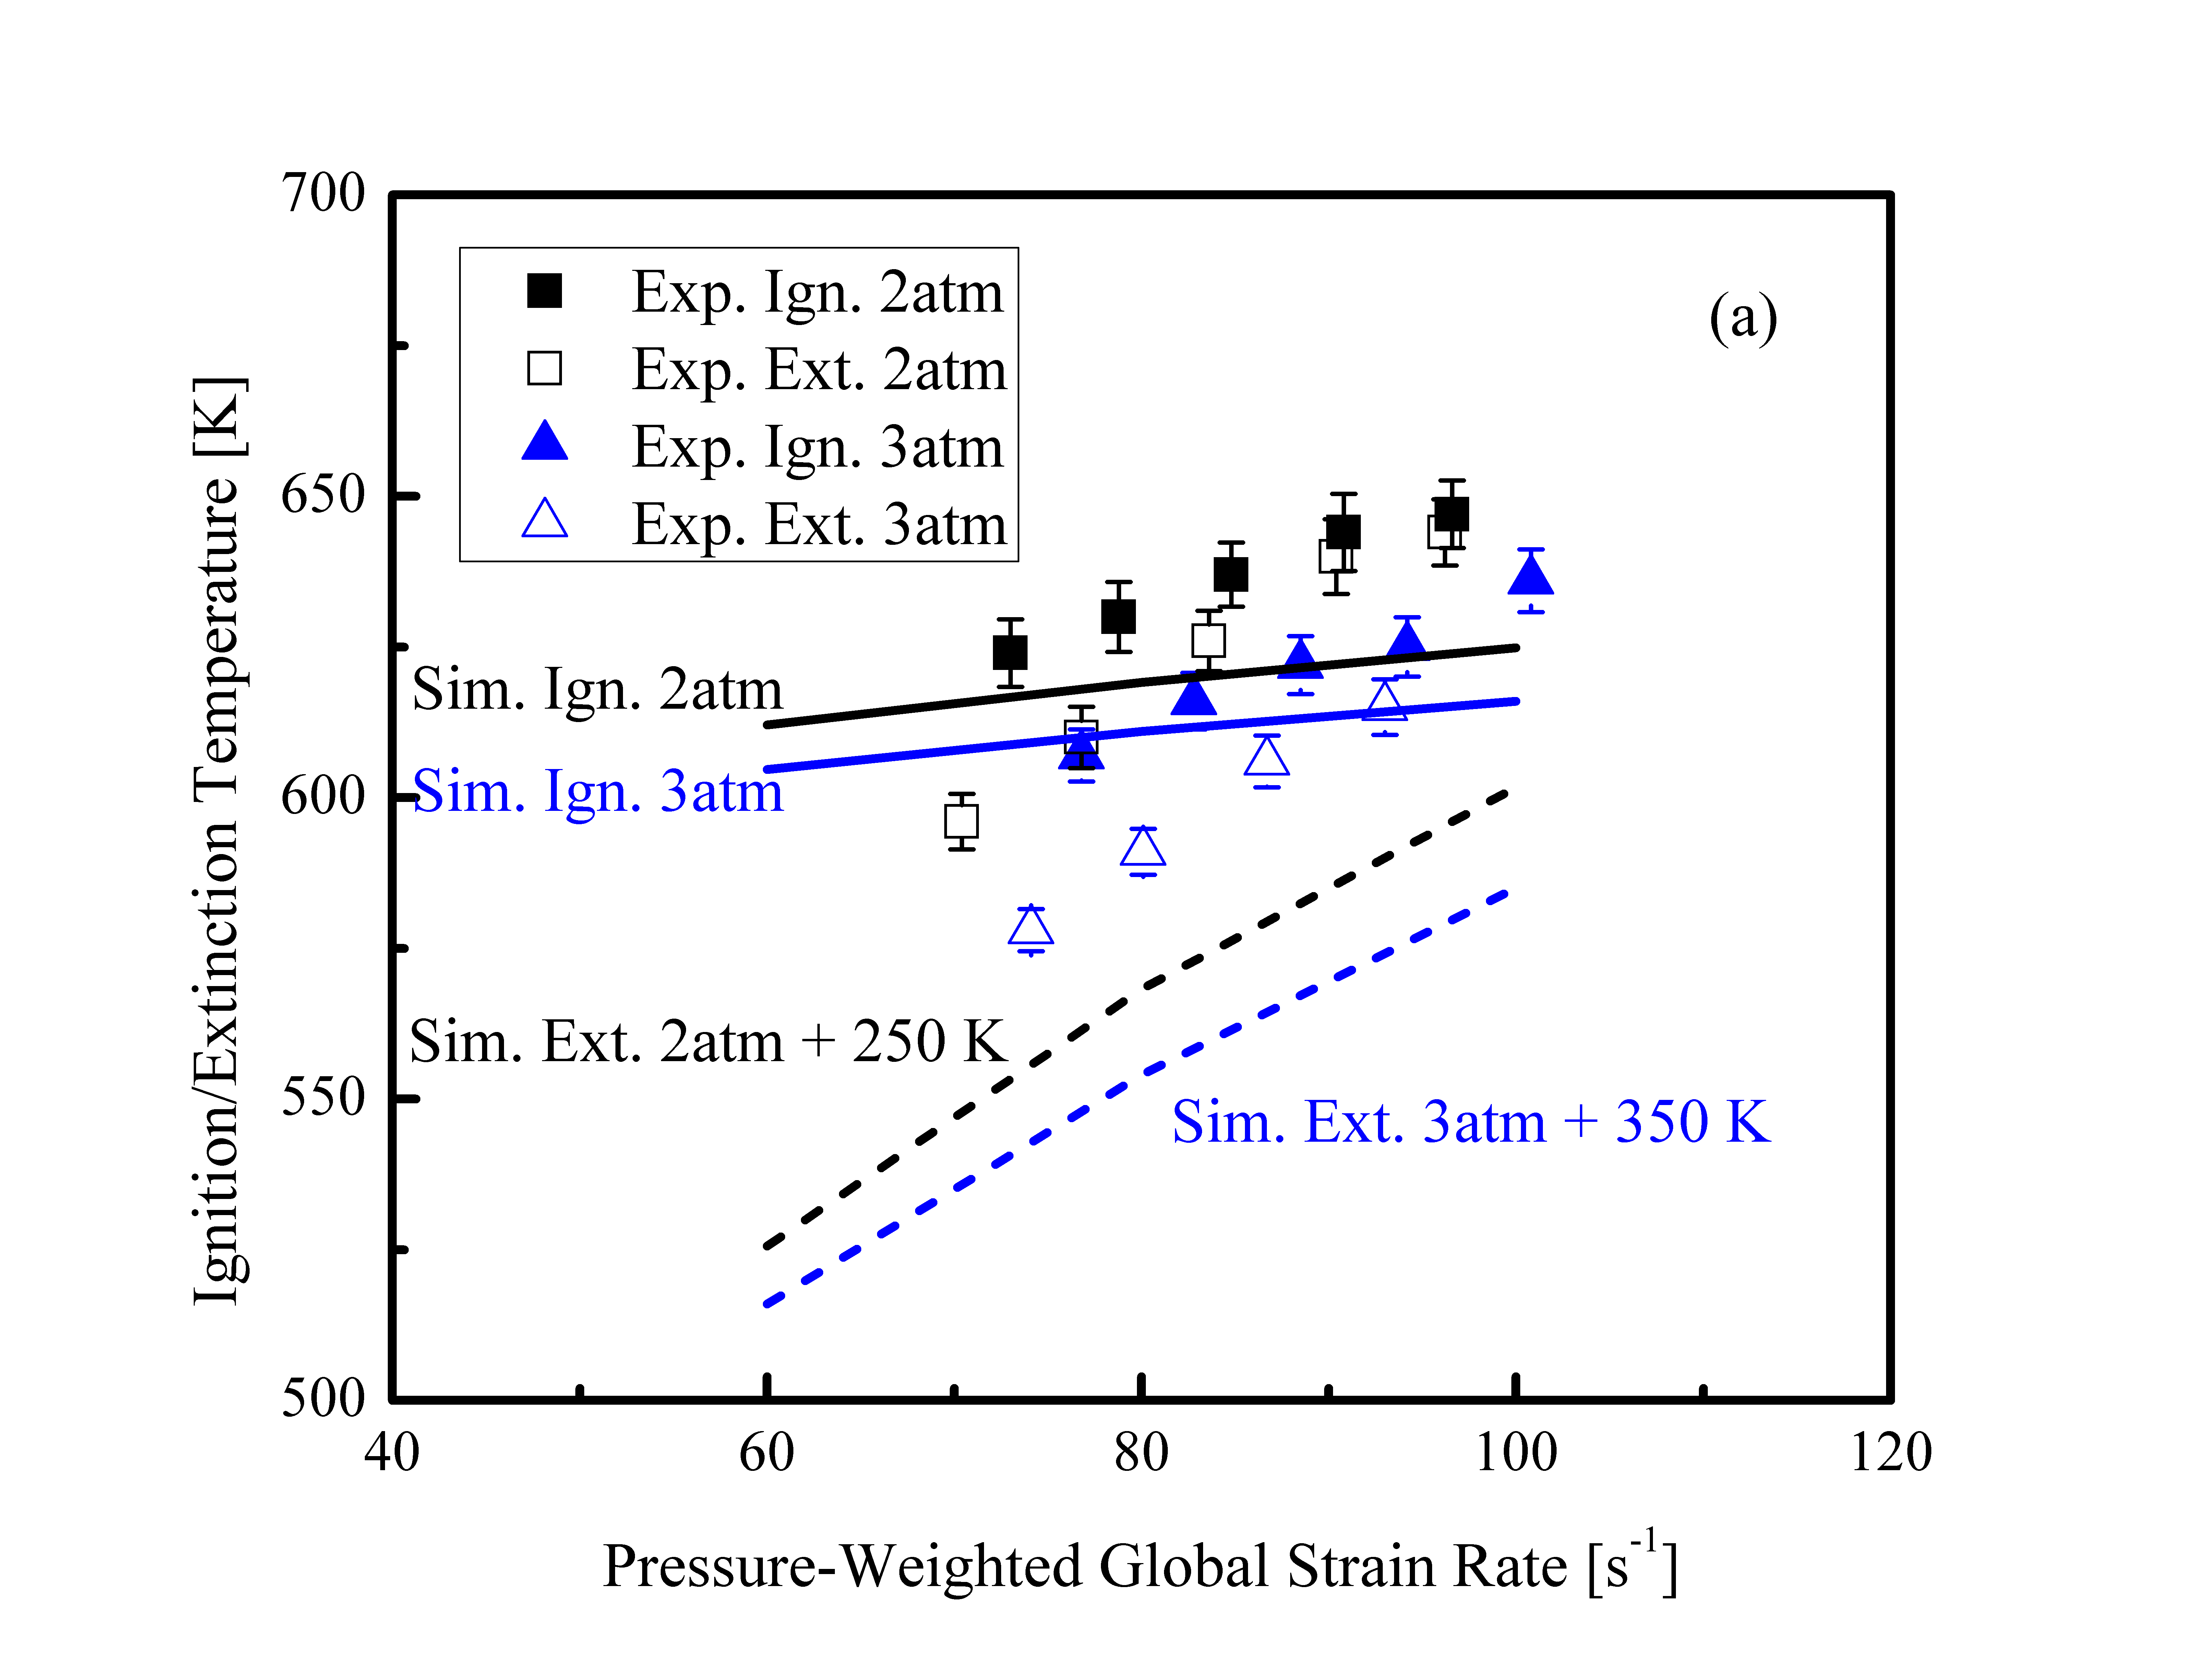
\includegraphics[width=1.0\textwidth]{ch-NTC/cmp_P.png}
  \normalsize
  \caption{Ignition and extinction temperatures at various strain rates and pressures in experiments and computations with the original chemical model.  Some of the computed extinction temperatures are shifted up for better illustration.  DME volume fraction in the fuel stream is 50\%, and the oxidizer stream is air.}
  \label{fig:cmp_P_ori}
\end{figure}

The conclusion that elevated pressure promotes low-temperature chemistry is consistent with previous studies with $n$-heptane~\cite{law12}.  Such promotion effect can be explained with the sensitivity analysis in Sec.~\ref{sec:NTC-structure}.  Qualitatively, sensitivity analysis conducted for elevated pressures shows similar dominant chemical pathways as Fig.~\ref{fig:NTC-SA}.  At elevated pressures, the balance of the reaction $\rm{CH}_2\rm{OCH}_2\rm{O}_2\rm{H} + \rm{O}_2 \Longleftrightarrow \rm{O}_2\rm{CH}_2\rm{OCH}_2\rm{O}_2\rm{H}$ shifts forward and promotes the formation of the important intermediate radicals for low-temperature chemistry.  Moreover, the $\rm{CH}_2\rm{OCH}_2\rm{O}_2\rm{H} \Longleftrightarrow \rm{OH} + 2\rm{CH}_2\rm{O}$ reaction is retarded at elevated pressures.

\begin{figure}[t]
  \centering
  \scriptsize
  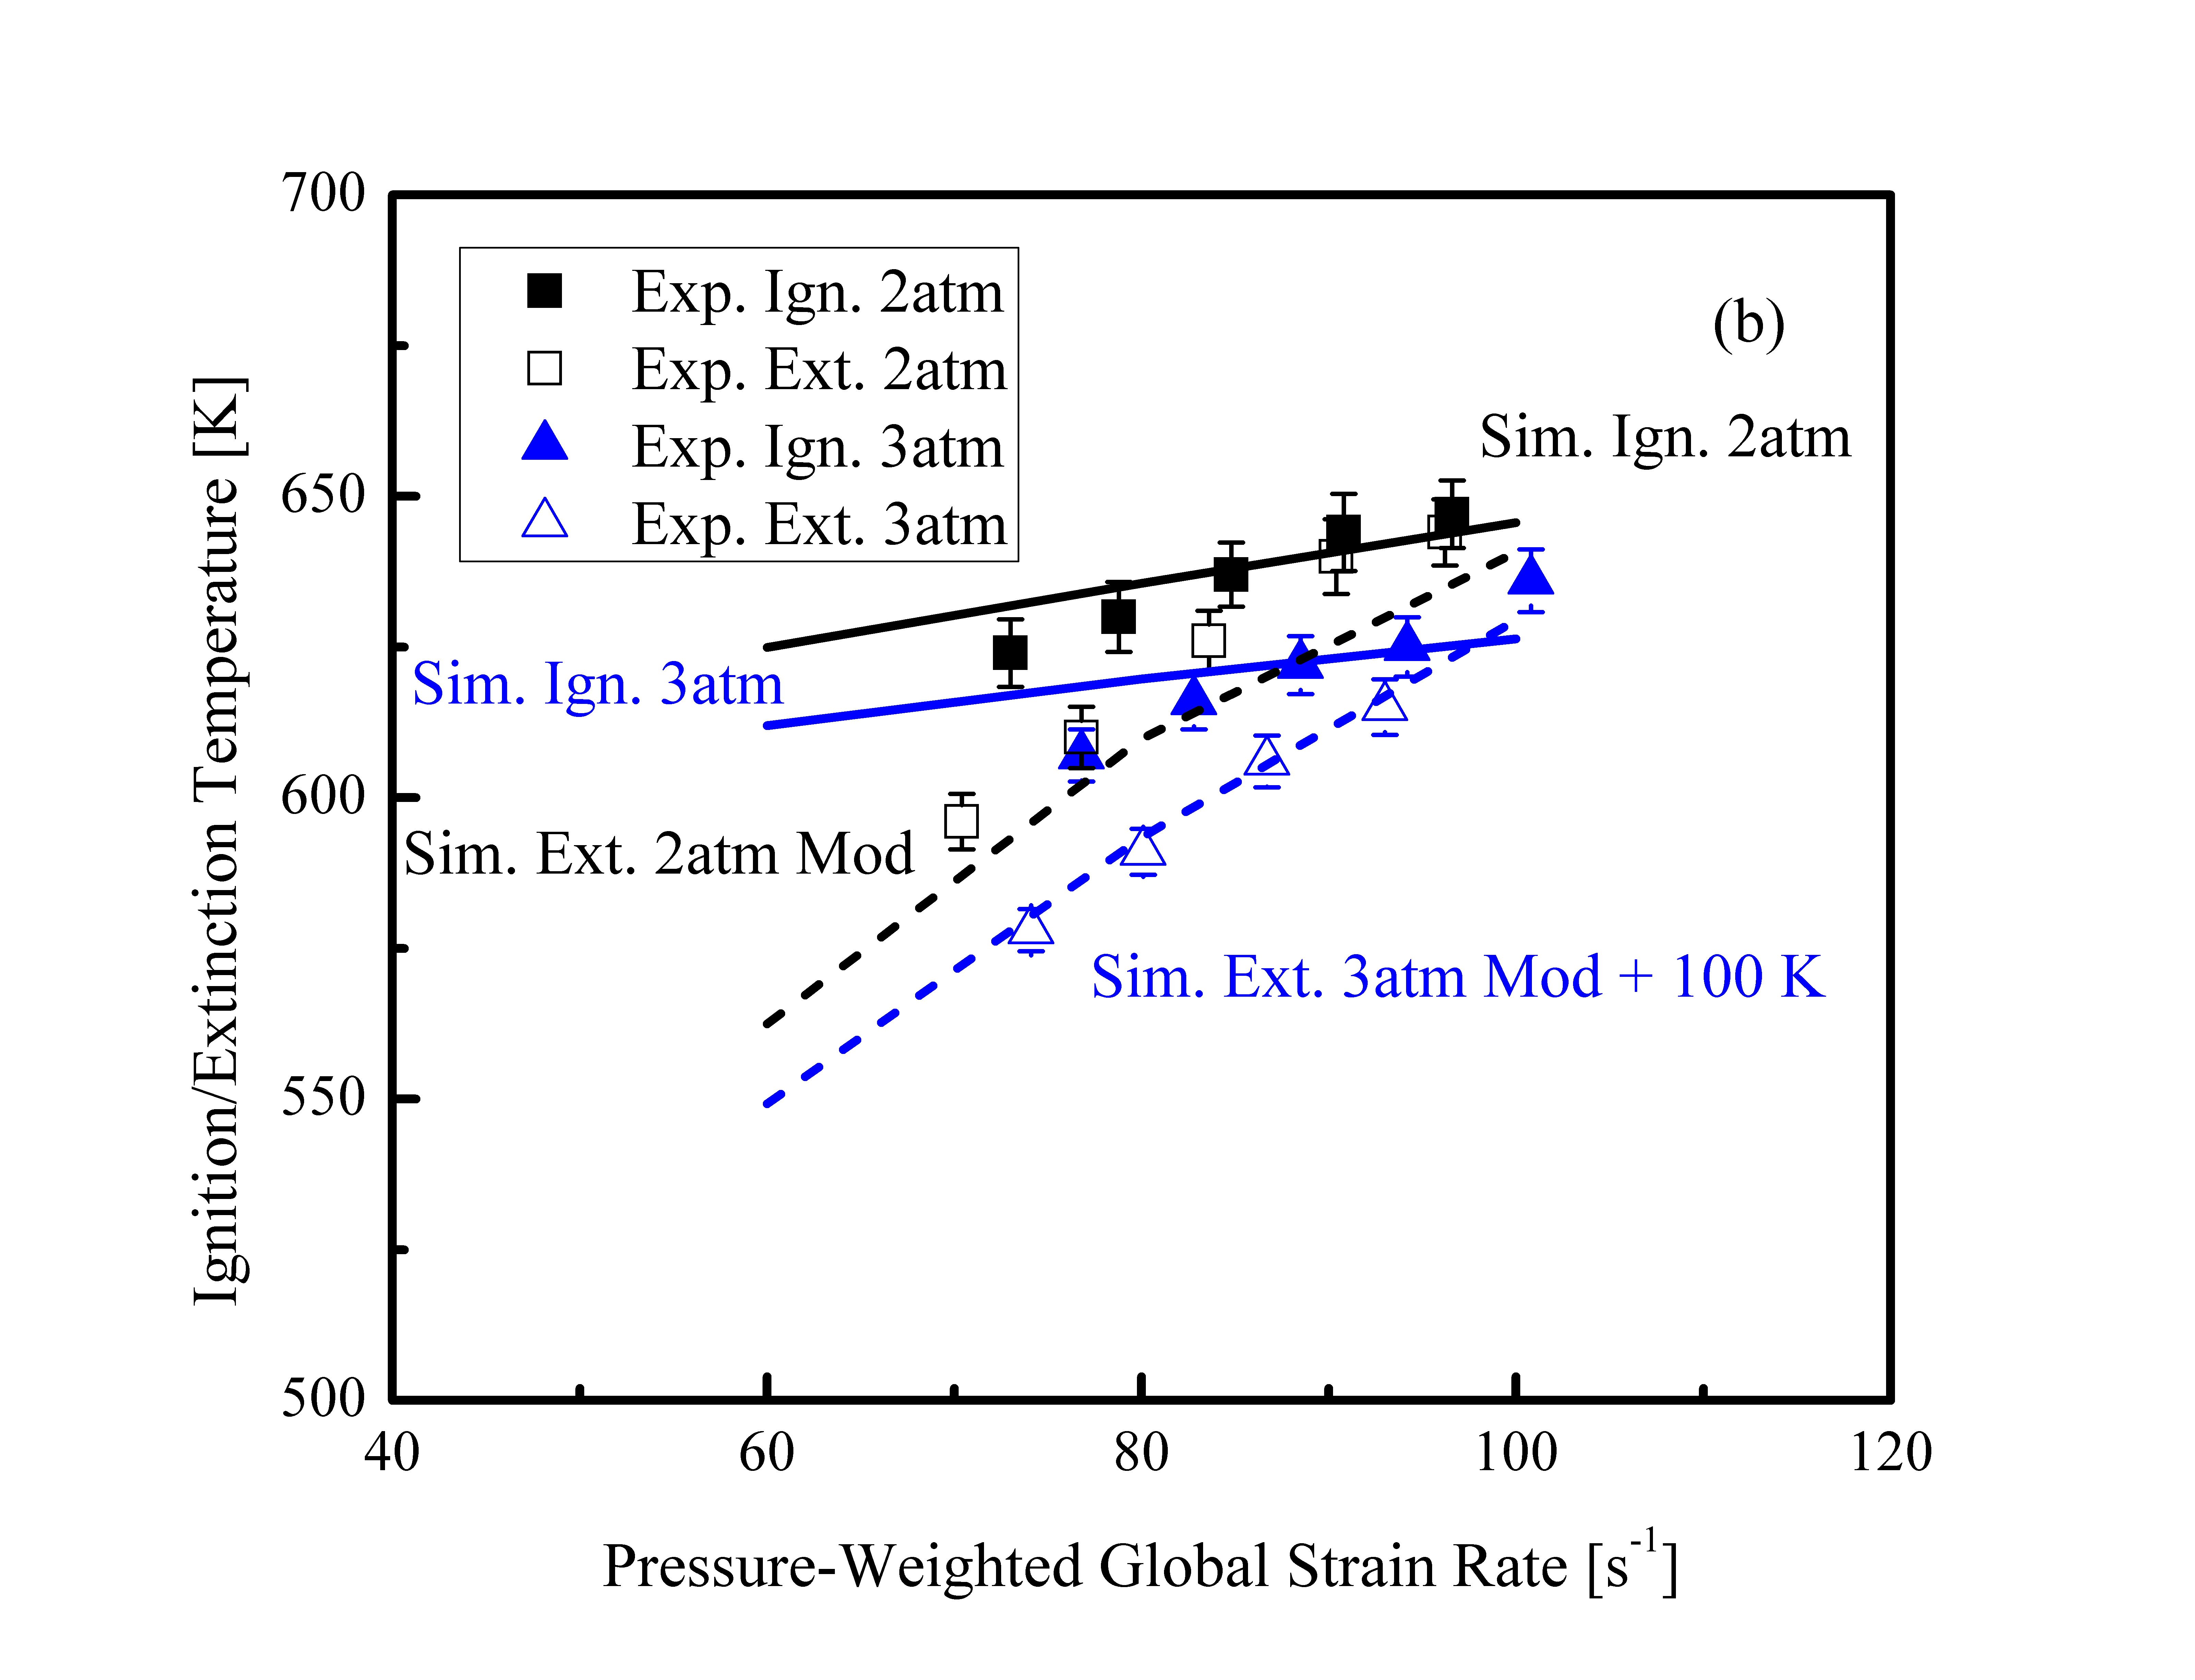
\includegraphics[width=1.0\textwidth]{ch-NTC/cmp_P_mod.png}
  \normalsize
  \caption{Ignition and extinction temperatures at various strain rates and pressures in experiments and computations with the modified chemical models.  Some of the computed extinction temperatures are shifted up for better illustration.  DME volume fraction in the fuel stream is 50\%, and the oxidizer stream is air.}
  \label{fig:cmp_P_mod}
\end{figure}

Figures~\ref{fig:cmp_P_ori} and~\ref{fig:cmp_P_mod} further show that the experimental ignition and extinction temperatures decrease at elevated pressures.  It is seen that while the effects of elevated pressure on ignition temperatures are predicted by computations qualitatively, the effects on extinction temperatures are significantly overpredicted when using the original mechanism (Fig.~\ref{fig:cmp_P_ori}).  The comparison is improved by using the two modified reactions (Fig.~\ref{fig:cmp_P_mod}), although the degree of improvement is less satisfactory as for the case of 2 atm pressure, shown in Fig.~\ref{fig:cmp_demo_mod}. It is emphasized again that it is preferred that the comparison is left as is, without further “tuning” the reactions as it does not seem to be justified within the scope of the present study. 

\begin{figure}[t]
  \centering
  \scriptsize
  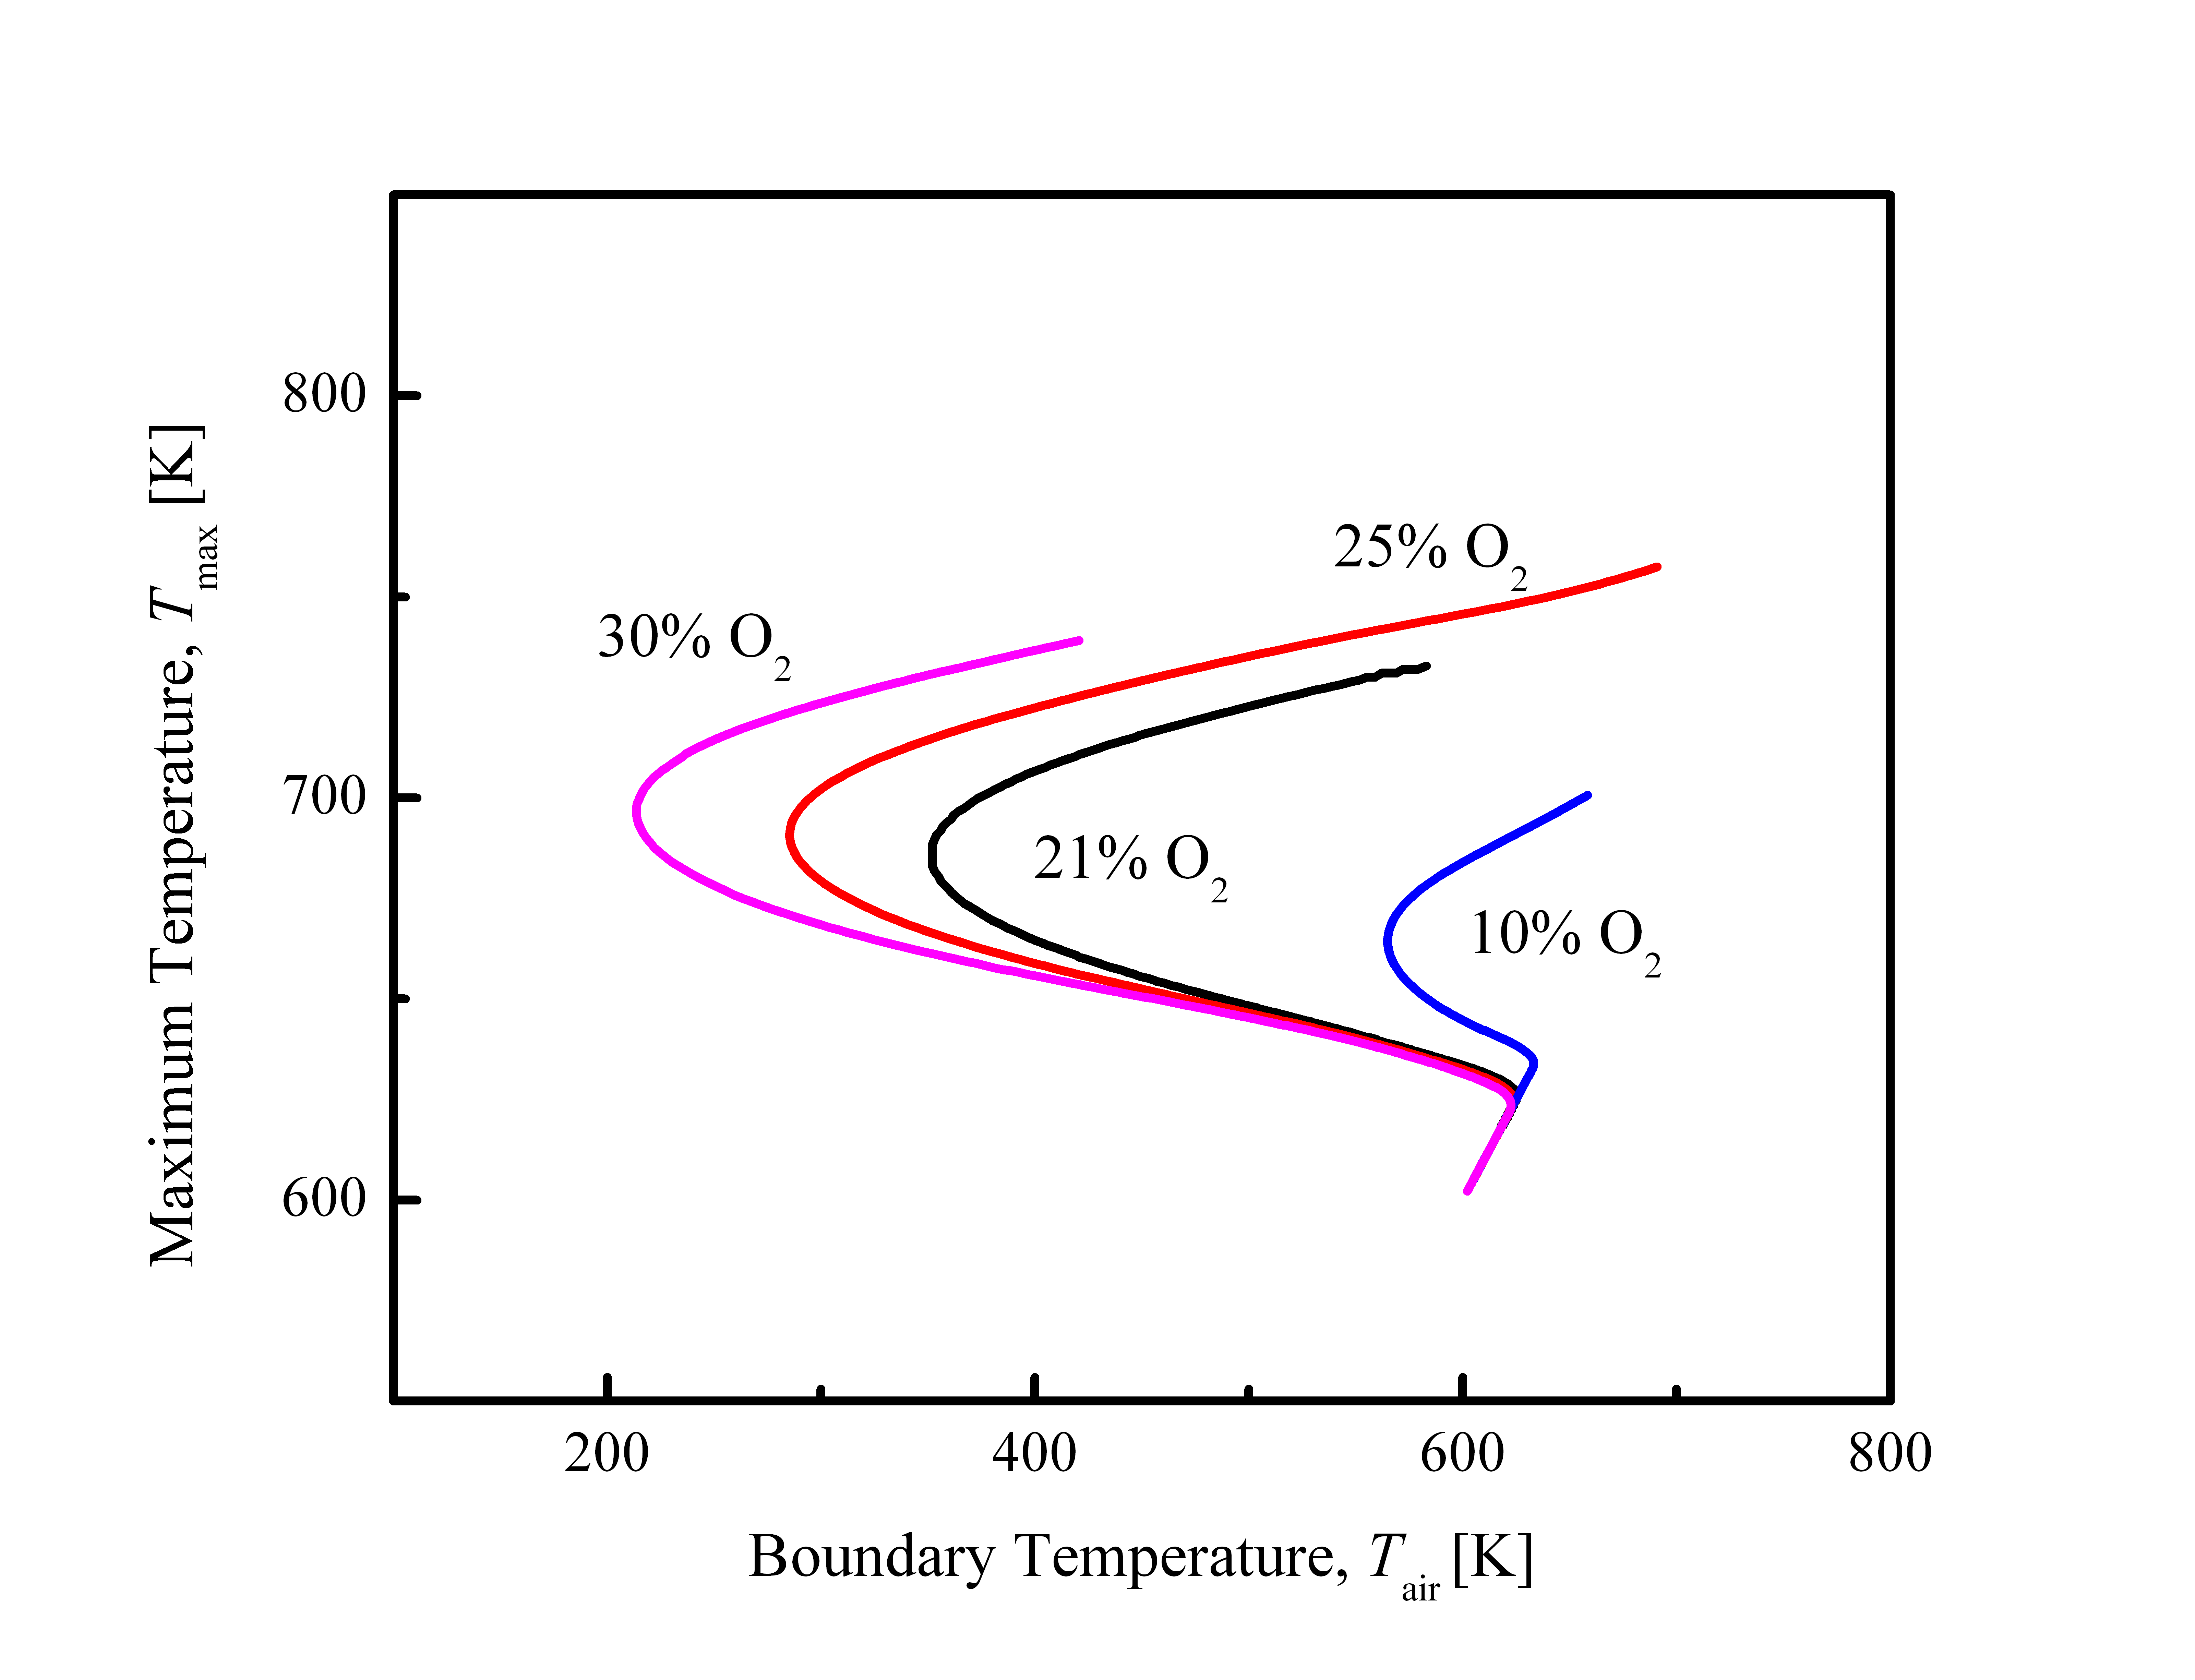
\includegraphics[width=1.0\textwidth]{ch-NTC/eff_O2.png}
  \normalsize
  \caption{S-curve analysis for various oxygen concentrations and the pressure-weighted strain rate of 100 /s.  DME volume fraction in the fuel stream is 50\%, and the ambient pressure is 2 atm.}
  \label{fig:eff_O2}
\end{figure}

Figure~\ref{fig:eff_O2} shows that increasing the oxygen concentration extends the hysteresis temperature window of the cool flame at the same ambient pressure and strain rate, while the ignition temperature is almost unaffected except at very low concentrations.  This is because, with increased oxygen concentration and hence decreased inert concentration, the heat release from the cool flame becomes more pronounced, which results in decreased extinction temperature.  Dominant chemical pathways for these conditions are similar to those in Fig.~\ref{fig:NTC-SA}.

\begin{figure}[t]
  \centering
  \scriptsize
  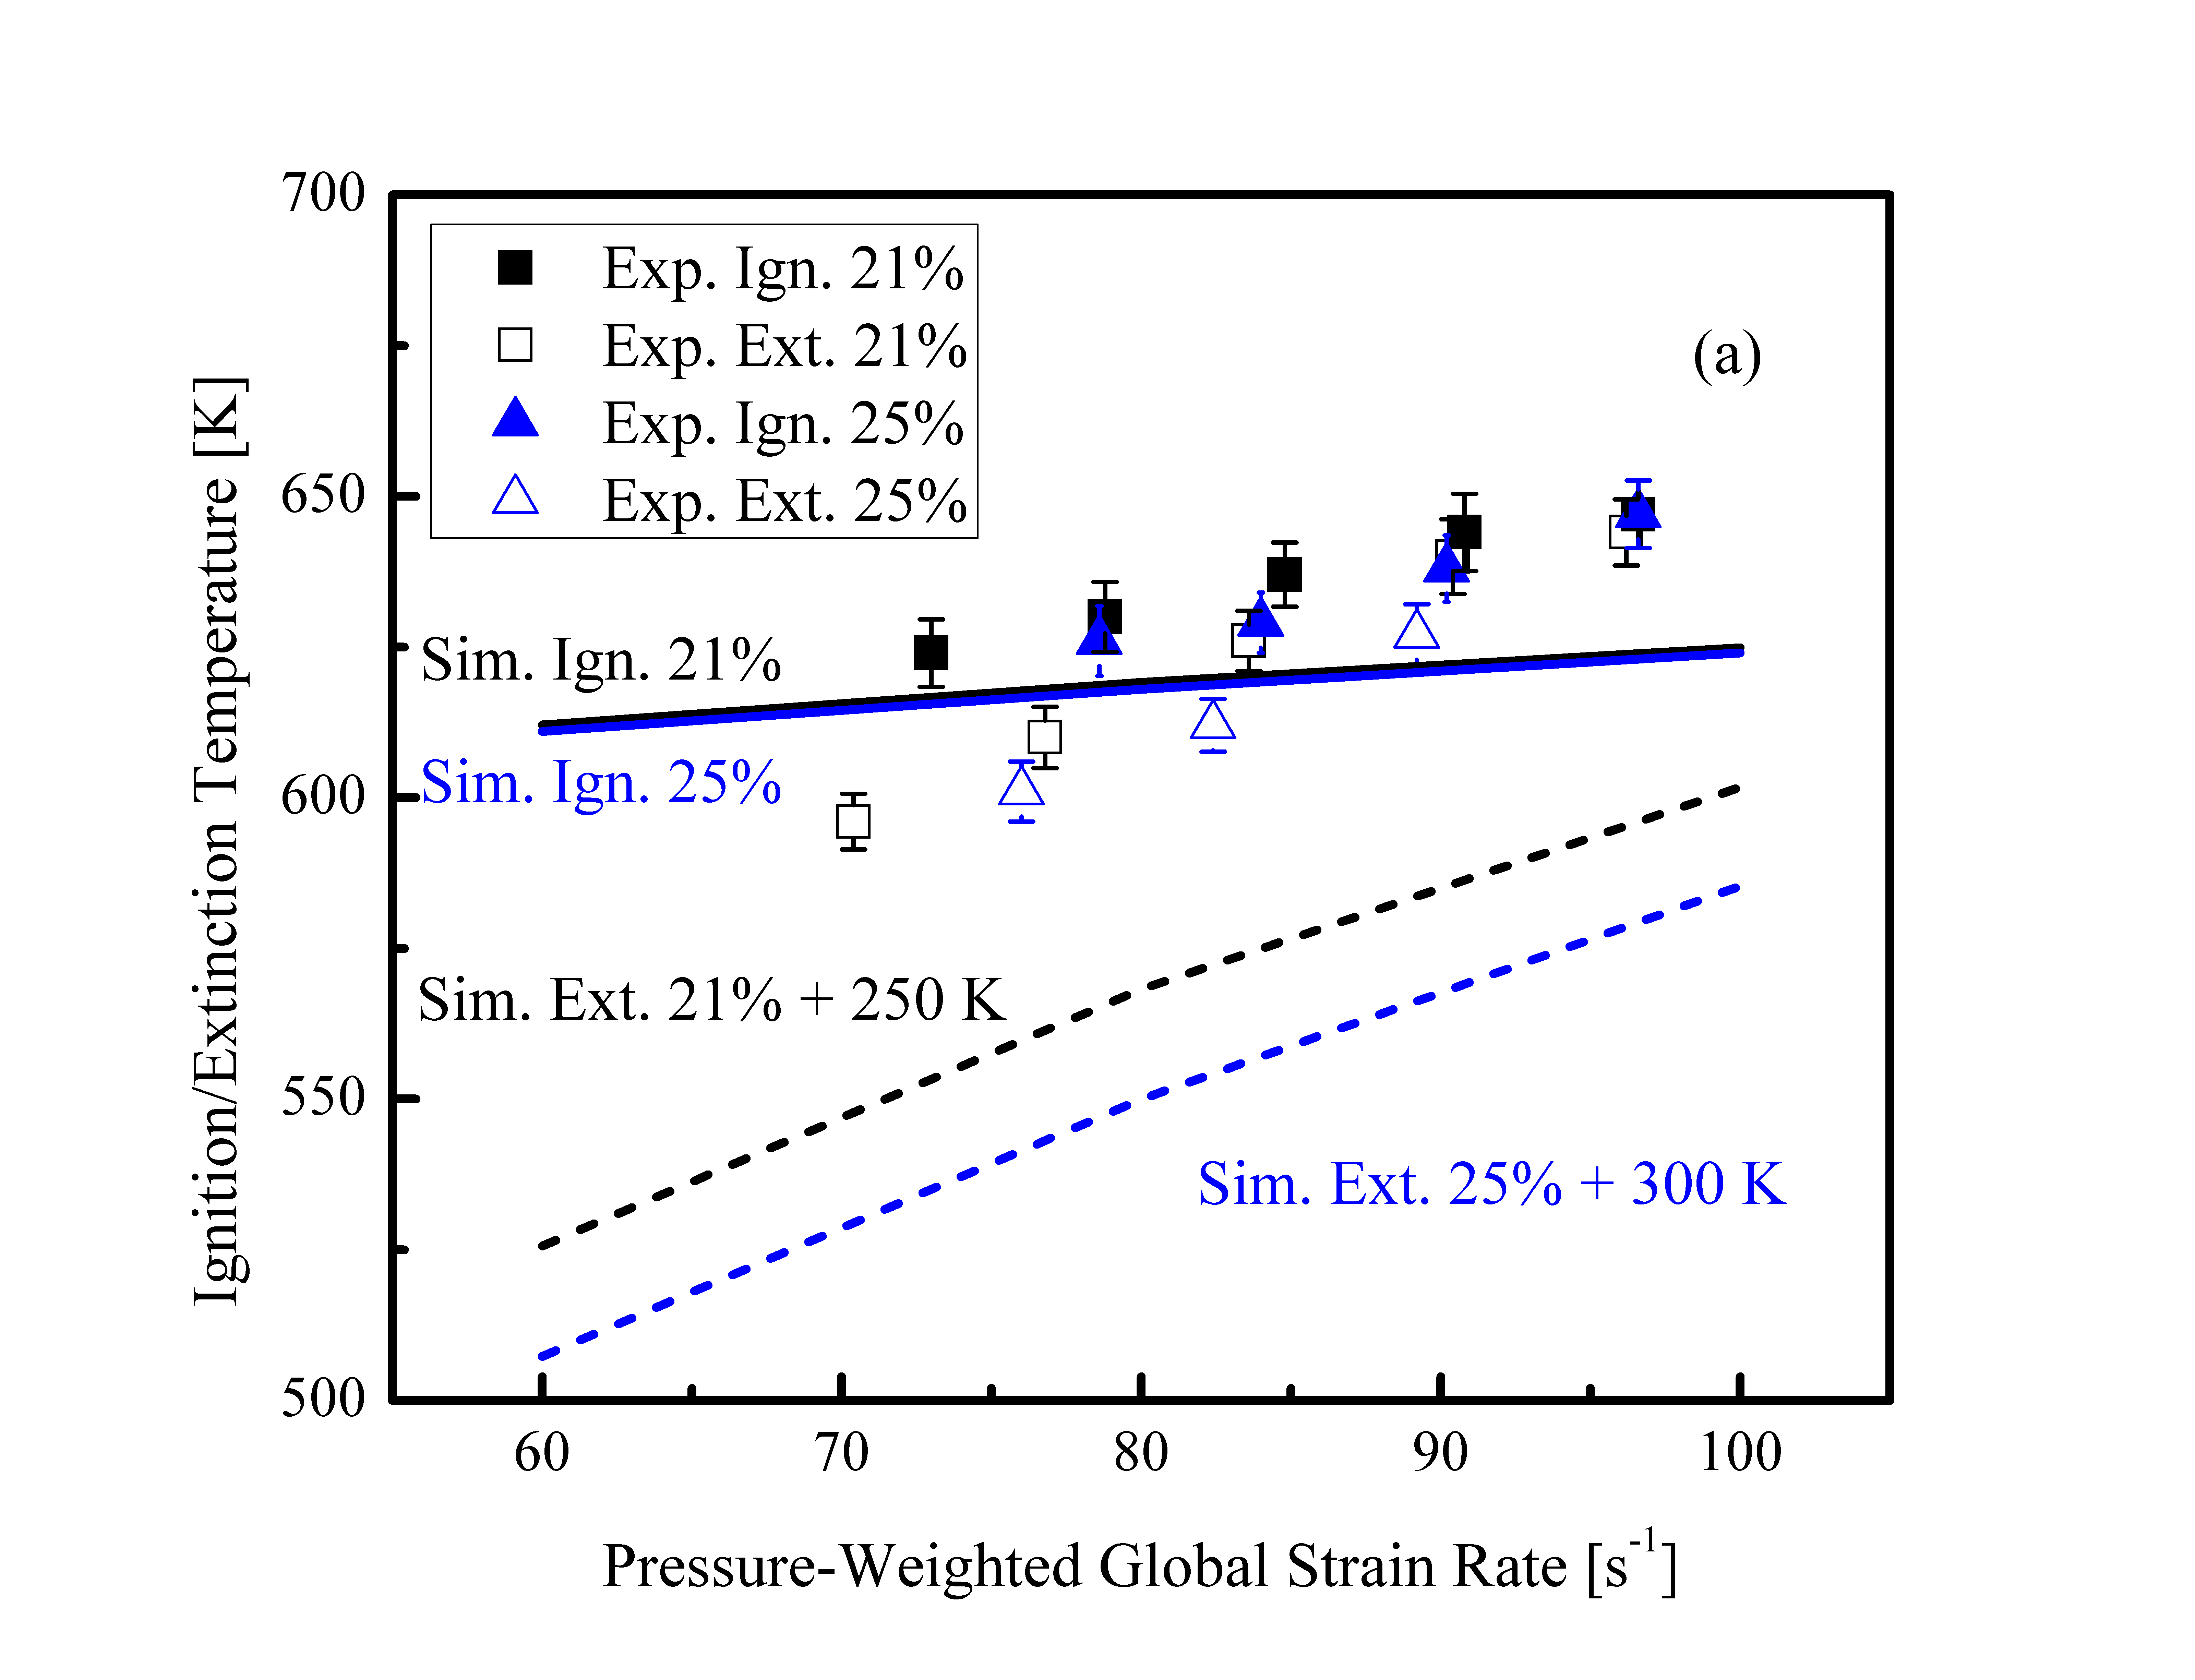
\includegraphics[width=1.0\textwidth]{ch-NTC/cmp_O2.png}
  \normalsize
  \caption{Ignition and extinction temperatures at various strain rates and oxygen concentrations in experiments and computations with the original chemical model.  Some of the computed extinction temperatures are shifted up for better illustration.  DME volume fraction in the fuel stream is 50\%, and the ambient pressure is 2 atm.}
  \label{fig:cmp_O2_ori}
\end{figure}  

The insensitivity of the cool flame ignition temperature is further confirmed with the experimental measurements, as shown in Fig.~\ref{fig:cmp_O2_ori}.  However, the reduction effect of increased oxygen concentration on the cool flame extinction temperature is again overpredicted by the computation, while improved agreements are achieved with the two modified preexponential factors (Fig.~\ref{fig:cmp_O2_mod}).

\begin{figure}[t]
  \centering
  \scriptsize
  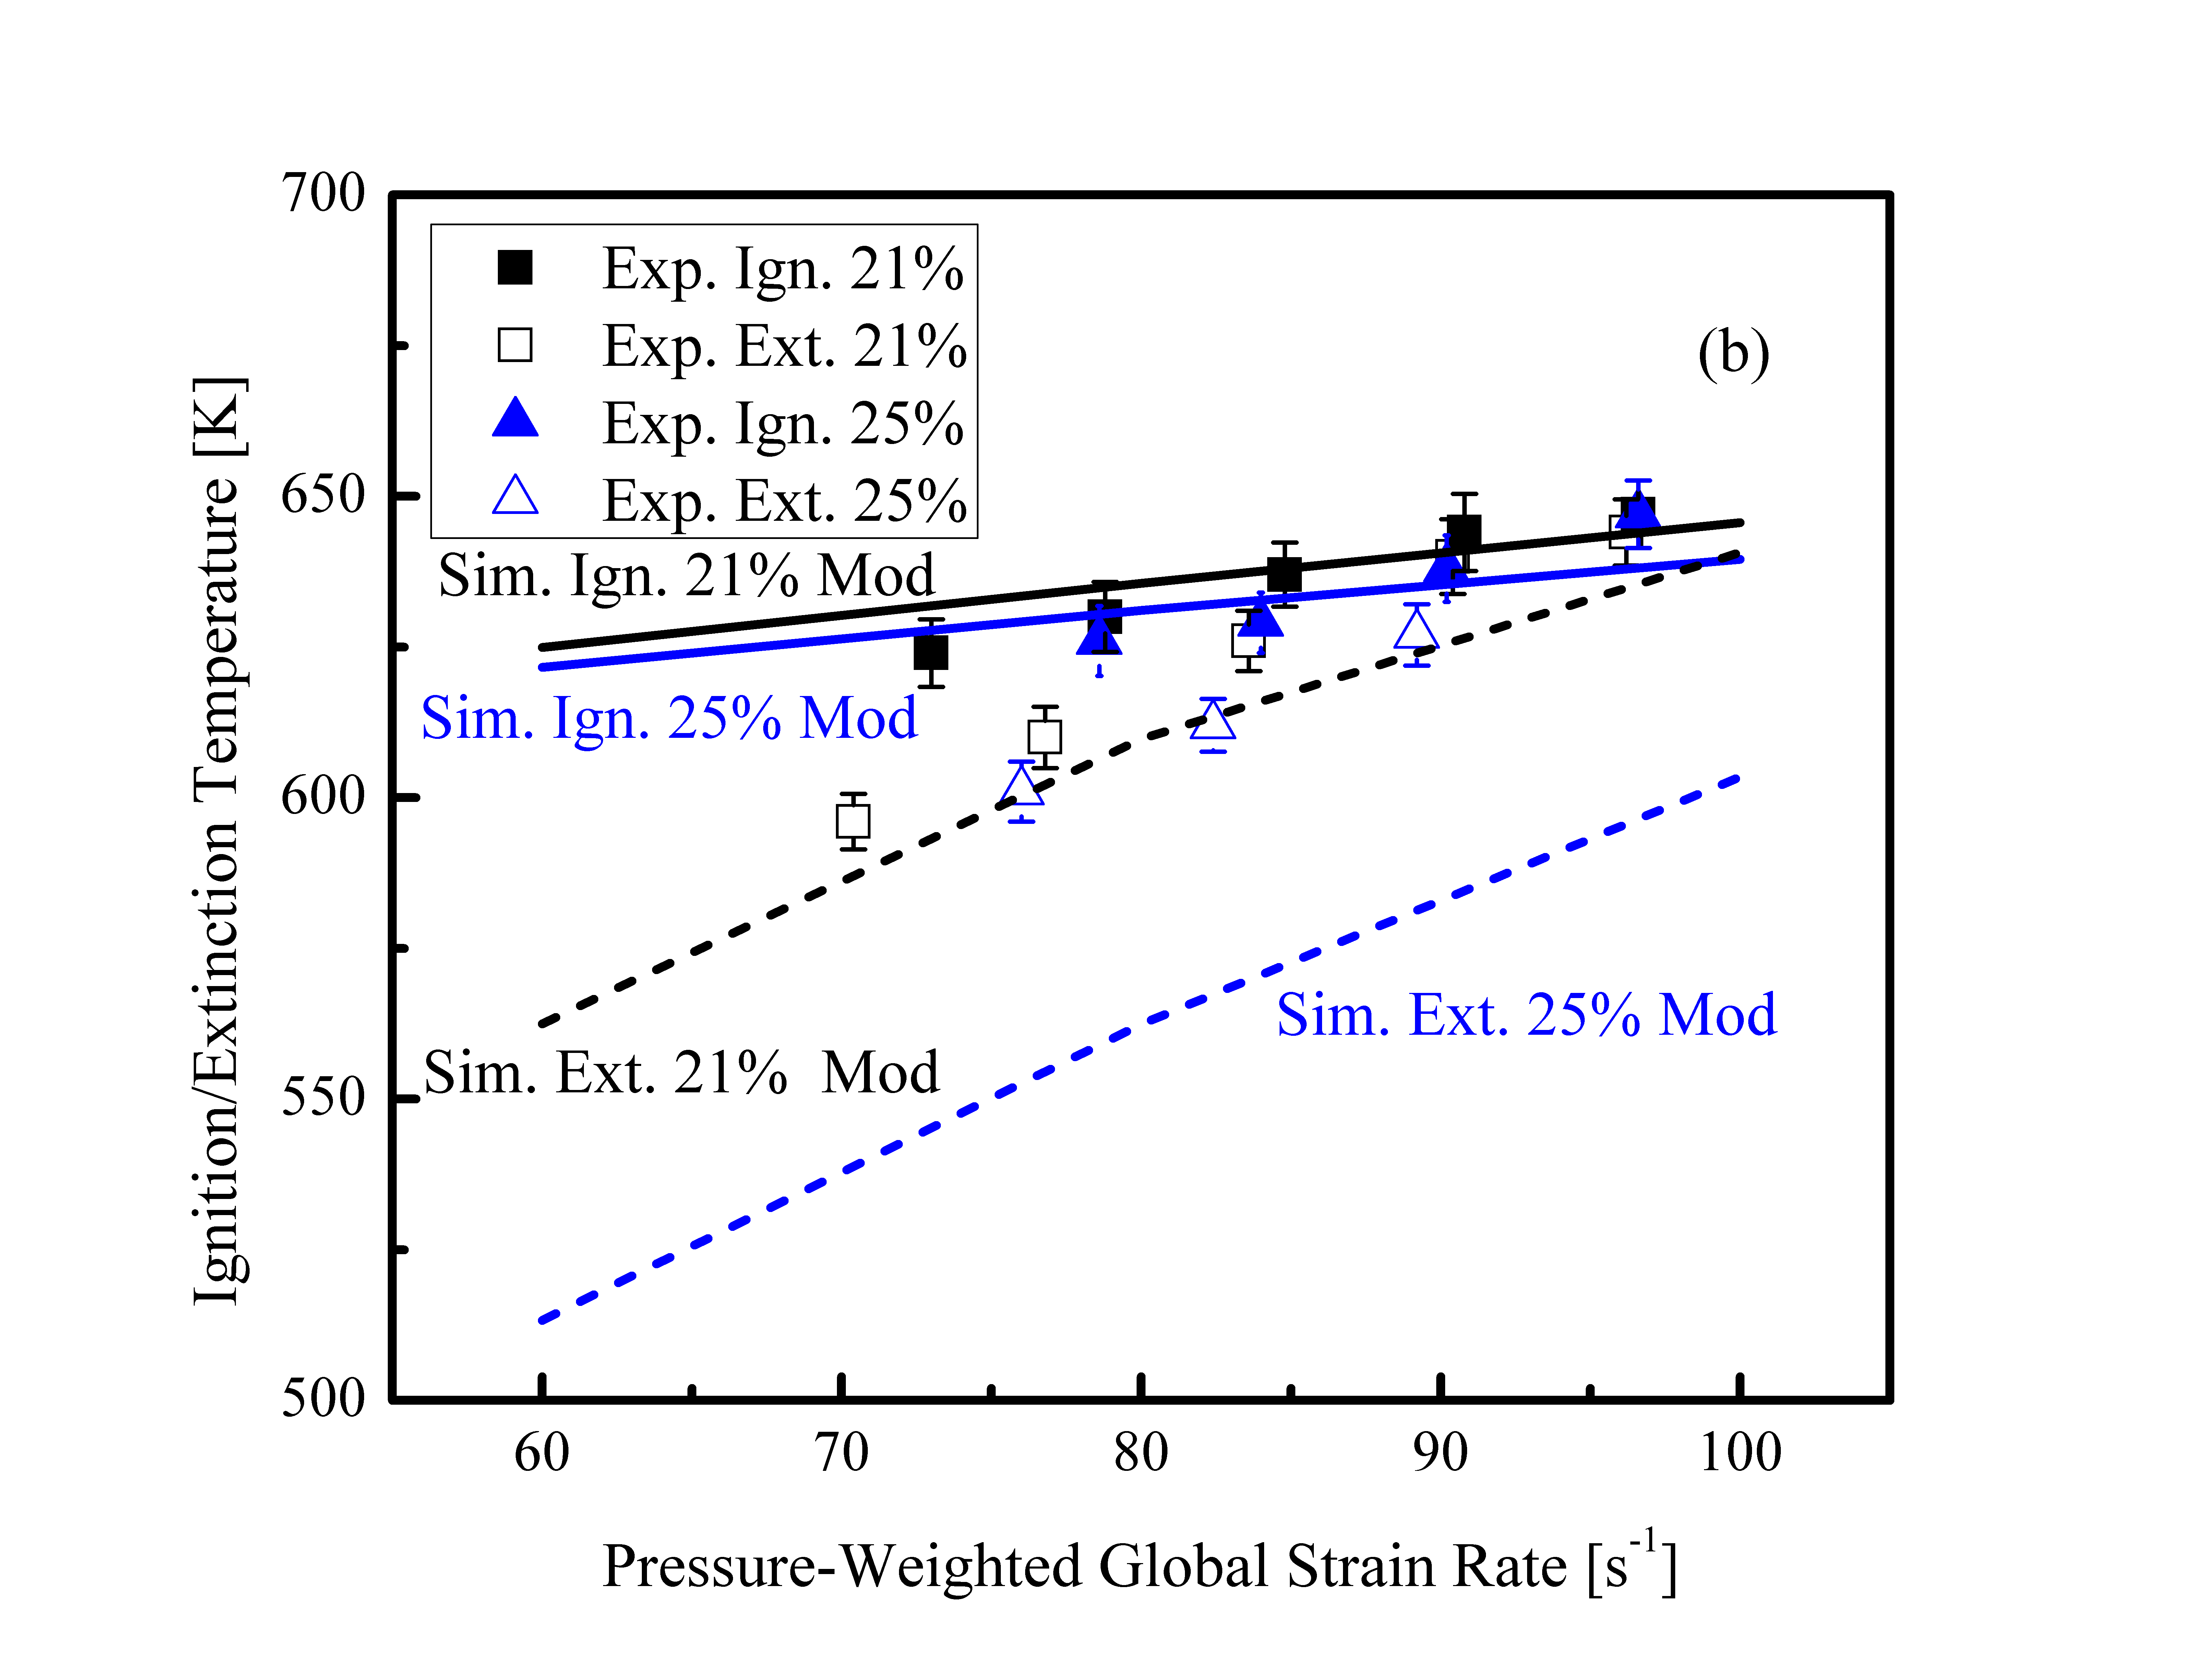
\includegraphics[width=1.0\textwidth]{ch-NTC/cmp_O2_mod.png}
  \normalsize
  \caption{Ignition and extinction temperatures at various strain rates and oxygen concentrations in experiments and computations with the modified chemical models.  Some of the computed extinction temperatures are shifted up for better illustration.  DME volume fraction in the fuel stream is 50\%, and the ambient pressure is 2 atm.}
  \label{fig:cmp_O2_mod}
\end{figure}

\section{Summary}

In this chapter, S-curve analysis was performed computationally to demonstrate the distinctive ignition and extinction states and structures of nonpremixed DME counterflow cool flames at various strain rates, ambient pressures, and fuel and oxidizer concentrations.  The design of the experimental counterpart to substantiate the computational investigation is very challenging due to the limited heat release and species production in cool flames and lack of robustness of such flames.  Qualitatively, the cool flame reactivity was substantiated with the ``M'' shaped signal captured by the PMT-oscilloscope system.  The ignition of the cool flame at atmospheric pressure was quantified with sensitive infrared imaging.  

Realizing that elevated pressure promotes cool flames and the limitation of the infrared experimental system, the detection method was improved with UV camera imaging.  The hysteretic ignition and extinction behavior of the nonpremixed cool flame was then observed and quantified in experiments for the first time.  It is noted, however, the extinction behavior of the cool flame was less well predicted by computation compared to ignition.  Possible reasons for such discrepancies were discussed, including experimental uncertainties and the high sensitivity in some reaction rates.  Although the objective of this chapter is not to propose an improved chemical model with modified kinetic parameters, it demonstrates the sensitive nature of the low-temperature chemistry, which stresses the need for further investigation on the low-temperature chemical kinetics. 
